\documentclass[12pt,a4paper]{report}

% ===== Font: Times New Roman (+ font matematico coerente) =====
\usepackage{mathptmx}

% ===== Lingua (rinomina "Chapter"->"Capitolo", "Contents"->"Indice", "Bibliography"->"Bibliografia") =====
% Sul server manca texlive-lang-italian (italian.ldf): babel carica l'italiano dal suo file .ini.
% Installato il pacchetto, si può tornare a \usepackage[italian]{babel}.
\usepackage{babel}
\babelprovide[import, main]{italian}

% ===== Margini: 2,5 cm su tutti i lati =====
\usepackage[left=2.5cm,right=2.5cm,top=2.5cm,bottom=2.5cm]{geometry}

% ===== Interlinea 1,5 =====
\usepackage{setspace}
\setstretch{1.5}

% ===== Immagini =====
\usepackage{graphicx}
\usepackage{float} % posiziona figure/tabelle esattamente dove sono nel sorgente (placement [H])
\usepackage{amsmath}
\usepackage{booktabs}
\usepackage{tikz}
\usepackage{tabularx}
\usepackage{array}
\usepackage{pgfplots}
\pgfplotsset{compat=1.18}
\usepgfplotslibrary{groupplots}
\newcolumntype{L}[1]{>{\raggedright\arraybackslash}p{#1}}
\newcolumntype{C}[1]{>{\centering\arraybackslash}p{#1}}
\newcolumntype{X}{>{\raggedright\arraybackslash}X}
\usepackage{geometry}
\geometry{a4paper, margin=1in}
\usetikzlibrary{arrows.meta, positioning, fit, backgrounds, calc, shapes.geometric, shapes.callouts}

% ===== Codice sorgente: monospace 10pt con syntax highlighting =====
\usepackage{xcolor}
\usepackage{listings}
\lstset{
    basicstyle=\ttfamily\fontsize{10}{12}\selectfont,
    keywordstyle=\color{blue}\bfseries,
    commentstyle=\color{gray}\itshape,
    stringstyle=\color{teal},
    breaklines=true,
    showstringspaces=false,
    frame=single,
    numbers=left,
    numberstyle=\tiny\color{gray},
    captionpos=b,
}

% ===== Collegamenti ipertestuali (indice, riferimenti, citazioni) =====
\usepackage{hyperref}

\title{[Titolo provvisorio della tesi]}
\author{[Nome Cognome]}
\date{[Anno Accademico]}

\begin{document}

% ===== Frontespizio =====
\begin{titlepage}
    \centering
    \vspace*{1cm}
    {\large Università di Bologna}\\[0.3cm]
    {\large Ingegneria e scienze informatiche}\\[2cm]

    {\Huge \bfseries Assistente Universitario}\\[3cm]

    \begin{minipage}{0.45\textwidth}
        \raggedright
        \large Relatore:\\
        Matteo Ferrara
    \end{minipage}
    \hfill
    \begin{minipage}{0.45\textwidth}
        \raggedleft
        \large Candidato:\\
        Michele Nardini
    \end{minipage}

    \vfill
    {\large Anno Accademico [2025/2026]}
\end{titlepage}

% ===== Numerazione pagine: frontespizio escluso, indice in numeri romani =====
\pagenumbering{roman}
\tableofcontents

% ===== Numerazione araba a partire dall'Introduzione =====
\pagenumbering{arabic}
\setcounter{page}{1}

% ===== Capitoli =====
\chapter{Introduzione}

Il sito web e la documentazione di un ateneo raccolgono un’enorme quantità di informazioni — regolamenti, tasse, scadenze, piani di studio, materiali didattici — ma lo fanno in modo estremamente dispersivo: argomenti correlati tra loro si trovano su pagine diverse, i documenti sono distribuiti in sezioni distinte del sito senza un percorso di consultazione unico, e le informazioni cambiano da un anno accademico all’altro senza che sia sempre immediato capire dove si trovi la versione aggiornata. Uno studente che cerca una risposta rapida a una domanda deve spesso incrociare più fonti per ricostruire un quadro coerente, con un dispendio di tempo non indifferente e un rischio concreto di interpretazioni errate. Quando questo non basta, lo studente è costretto a rivolgersi direttamente agli uffici amministrativi, che ricevono così un flusso costante di richieste ripetitive, spesso relative a informazioni già pubblicate ma difficili da reperire. Un assistente in grado di rispondere a queste domande attingendo alle fonti ufficiali potrebbe quindi alleggerire in modo significativo il carico di lavoro del personale amministrativo, oltre a ridurre i tempi di attesa per gli studenti.

A questa dispersione si aggiunge una seconda difficoltà, che riguarda gli studenti che per ragioni diverse faticano a
seguire le lezioni con regolarità: per loro, un assistente capace di rispondere anche su contenuti didattici --- non
solo su procedure amministrative --- rappresenta un supporto concreto per recuperare e comprendere quanto trattato a
lezione, anche senza avervi potuto assistere di persona. Lo stesso tipo di supporto porta con sé un beneficio
speculare per i docenti: chi tiene più corsi, spesso con un numero elevato di studenti iscritti, fatica a propria
volta a rispondere individualmente a tutte le domande che riceve, molte delle quali ricorrenti e già risposte in
precedenza ad altri studenti. Un assistente che risponde autonomamente alle domande più comuni alleggerisce questo
carico, lasciando ai docenti le domande che richiedono davvero la loro attenzione diretta.

La soluzione proposta in questo lavoro di tesi è un assistente conversazionale basato sul paradigma del
\emph{Retrieval-Augmented Generation} (RAG). A fronte di una domanda posta in linguaggio naturale, il sistema
recupera automaticamente, tra tutta la documentazione e il materiale didattico indicizzato, i frammenti più
pertinenti alla domanda posta, e li fornisce a un modello linguistico incaricato di formulare una risposta diretta
basandosi su di essi, citando la fonte da cui ogni affermazione proviene. In questo modo chi pone la domanda --- sia
esso uno studente o un docente che voglia verificare rapidamente un'informazione --- non deve più cercare manualmente
tra le pagine del sito o i materiali del corso: riceve una risposta puntuale e, soprattutto, verificabile, perché
ancorata a documenti reali e non semplicemente generata liberamente dal modello.

Il presente lavoro ha natura di \textbf{studio di fattibilità}: l'obiettivo primario non è consegnare un sistema
pronto per il deployment in produzione, ma verificare se un assistente di questo tipo --- completamente locale,
vincolato a un hardware non professionale --- possa rispondere con una qualità sufficiente a domande reali in questo
dominio, e individuare concretamente quelli che sono i limiti del sistema.

Il resto di questo lavoro di tesi è organizzato come segue. Il Capitolo~\ref{cap:stato_arte} inquadra il problema
nella letteratura esistente, introduce i concetti alla base dei modelli linguistici di grandi dimensioni e del
paradigma RAG, e passa in rassegna sistemi esistenti che affrontano problemi analoghi in ambito universitario. Il
Capitolo~\ref{cap:architettura} discute i vincoli di progetto che hanno guidato le scelte realizzative e descrive in
dettaglio l'architettura del sistema sviluppato, le scelte tecnologiche operate per ciascun componente e le
problematiche concrete incontrate durante lo sviluppo, insieme alle soluzioni adottate per risolverle. Il
Capitolo~\ref{cap:validazione} presenta la metodologia di valutazione sperimentale impiegata, gli esperimenti
condotti e i risultati ottenuti, inclusi alcuni casi di errore analizzati in dettaglio. Il
Capitolo~\ref{cap:conclusioni}, infine, riassume il contributo di questo lavoro rispetto agli obiettivi qui
enunciati, ne discute i limiti noti e ne delinea i possibili sviluppi futuri.



\chapter{Stato dell'arte}\label{cap:stato_arte}

Negli ultimi anni i modelli linguistici di grandi dimensioni (Large Language Model, LLM) si sono affermati come strumenti in grado di interpretare domande formulate in linguaggio naturale e di generare risposte fluenti e articolate, aprendo la strada a una nuova generazione di assistenti conversazionali. Queste capacità li rendono candidati naturali per un servizio di supporto agli studenti; tuttavia, utilizzati così come sono, i LLM presentano limiti che ne compromettono l’affidabilità proprio nei contesti in cui l’accuratezza dell’informazione è essenziale. Questo capitolo ripercorre lo stato dell’arte a partire da tali limiti, per poi presentare la Retrieval-Augmented Generation (RAG) come approccio pensato per superarli e descrivere le principali soluzioni proposte in letteratura.

\section{Limiti dei modelli linguistici in un dominio specifico}
\label{sec:problema}

Un modello linguistico di grandi dimensioni, per quanto addestrato su un corpus sterminato di testo, soffre di due limiti strutturali quando interrogato direttamente su un dominio specifico e circoscritto come quello universitario.

Il primo è la natura statica della sua conoscenza: i parametri del modello fissano ciò che esso ``sa'' al momento in cui l'addestramento si conclude, e qualunque informazione successiva a quella data come una nuova scadenza, un regolamento modificato, un importo delle tasse aggiornato, semplicemente non vi rientra. 
In \cite{zhao2023survey}, nella loro rassegna sui large language model, descrivono questo fenomeno con il termine \emph{outdatedness hallucination}: il modello genera un contenuto che era corretto al momento dell'addestramento ma non lo è più al momento dell'uso, senza alcun segnale esplicito che lo distingua da un'affermazione ancora valida, il modello stesso non ha modo di sapere che la propria conoscenza è invecchiata.

Il secondo limite riguarda l'assenza totale di accesso ai documenti specifici dell'istituzione interrogata: un LLM generico non ha mai visto i regolamenti di un ateneo, le pagine web di un singolo corso di laurea, le slide di un insegnamento particolare. Messo di fronte a una domanda che richiede questo tipo di conoscenza, non ha altra scelta che generalizzare da pattern appresi su domini affini o, più problematicamente, produrre una risposta sintatticamente corretta e sicura di sé ma priva di fondamento fattuale, un comportamento che prende il nome di \emph{hallucination}. Huang et al. \cite{huang2023survey} ne propongono una tassonomia sistematica, riconducendone le cause a limiti dei dati di addestramento (rumorosi, incompleti o distorti), a processi di allineamento che premiano risposte sicure più che corrette, e alla natura intrinsecamente stocastica del processo di
generazione del testo.

Questi due limiti si combinano in modo particolarmente dannoso nel dominio universitario, dove il costo di un errore non è astratto ma concreto e misurabile: una scadenza riportata in modo errato comporta una tassa pagata in ritardo, un requisito di ammissione frainteso comporta una domanda respinta. Kasneci et al. \cite{kasneci2023chatgpt}, discutendo opportunità e criticità dell'uso dei large language model in ambito educativo, osservano come l'assenza di garanzie sull'accuratezza fattuale sia uno degli ostacoli principali alla loro adozione diretta in contesti dove la correttezza dell'informazione fornita allo studente non è negoziabile.

La soluzione che la letteratura ha individuato per entrambi questi limiti consiste nel separare la conoscenza fattuale dal componente che genera il linguaggio: non chiedere al modello di ``ricordare'' un fatto a partire dai propri parametri, ma fornirglielo esplicitamente come contesto al momento della domanda, recuperandolo da una base documentale aggiornabile in modo indipendente dal modello stesso. È il principio alla base del Retrieval-Augmented Generation, discusso nella Sezione~\ref{sec:rag}, ed è il principio su cui si fonda l'intero sistema sviluppato in questo lavoro di tesi.

Questa non è l'unica strada percorribile: la conoscenza mancante di un LLM potrebbe, in linea di principio, essere aggiunta direttamente ai suoi parametri con un ulteriore addestramento mirato (\emph{fine-tuning}) sui documenti specifici del dominio, piuttosto che recuperata da una base esterna a ogni domanda. Ovadia et al. \cite{ovadia2024finetuning} confrontano empiricamente le due strade su compiti che richiedono conoscenza intensiva, sia per informazioni già presenti nei dati di addestramento sia per informazioni del tutto nuove, e osservano che il fine-tuning non supervisionato fatica sistematicamente ad apprendere fatti nuovi in modo affidabile --- a meno di esporre il modello a numerose riformulazioni dello stesso fatto durante l'addestramento, un costo che cresce con
ogni aggiornamento del documento sorgente --- mentre il RAG si dimostra costantemente più efficace in entrambi i casi. Per un dominio come quello universitario, dove i documenti cambiano ogni anno accademico, questo risultato ha un peso pratico diretto: un sistema a fine-tuning richiederebbe un nuovo ciclo di addestramento a ogni aggiornamento normativo, mentre un sistema RAG richiede solo di re-indicizzare il documento modificato.

Questo principio ha già trovato applicazione in sistemi conversazionali rivolti specificamente al contesto
universitario e industriale. Una presentazione più ampia di sistemi analoghi è presentata nella Sezione~\ref{sec:sistemi-simili}.

\section{Large Language Model (LLM)}\label{sec:llm}

\subsection{Che cos'è un LLM}

Un \emph{large language model} è, nella sua forma più diffusa, una rete neurale basata sull'architettura
\emph{Transformer} \cite{vaswani2017attention}, addestrata a predire il token successivo di una sequenza di testo a partire dai token che lo precedono. L'elemento che ha reso questa architettura dominante rispetto ai modelli ricorrenti che la precedevano è il meccanismo di \emph{self-attention}: ogni token della sequenza viene messo in relazione diretta con tutti gli altri, indipendentemente dalla loro distanza, e questo permette al modello di catturare dipendenze a lungo raggio nel testo senza il collo di bottiglia sequenziale delle reti ricorrenti. Soprattutto, la self-attention rende l'addestramento parallelizzabile su hardware specializzato, una condizione necessaria per scalare questi modelli alle dimensioni che oggi li caratterizzano, sia in termini di parametri sia di dati di addestramento.

% ---------------------------------------------------------------------------
% Tokenizzazione
% ---------------------------------------------------------------------------
Prima di poter essere elaborato da un LLM, il testo deve essere convertito in una sequenza di unità discrete, i \emph{token}. Un token non coincide necessariamente con una parola: le parole più frequenti corrispondono in genere a un singolo token, mentre quelle meno comuni vengono spezzate in più frammenti sub-lessicali, fino ad arrivare, nei casi limite, ai singoli caratteri. La segmentazione è stabilita da un \emph{tokenizer}, un algoritmo che apprende da un corpus di riferimento quali frammenti di testo ricorrono più spesso. Il più diffuso, il \emph{Byte-Pair Encoding} (BPE), parte dai singoli caratteri e fonde iterativamente le coppie di simboli adiacenti più frequenti, fino a costruire un vocabolario di dimensione prefissata, tipicamente dell'ordine di decine o centinaia di migliaia di token. Come illustra la Figura~\ref{fig:tokenizzazione}, a ogni token del vocabolario è associato un identificativo numerico, ed è questa sequenza di numeri, e non il testo, che il modello riceve in ingresso e produce in uscita. In questo modo un vocabolario finito è sufficiente a rappresentare qualunque testo, comprese parole mai incontrate durante l'addestramento.

La tokenizzazione ha una conseguenza pratica diretta: tutte le grandezze che caratterizzano un LLM sono misurate in token, non in parole o in caratteri. In particolare, la \emph{finestra di contesto}, ovvero il numero massimo di token che il modello può elaborare in un'unica interazione, prompt e risposta compresi, va da poche migliaia a centinaia di migliaia di token a seconda del modello, e pone un limite diretto alla quantità di testo recuperato (Sezione~\ref{sec:rag}) che può essere fornita come contesto per una singola domanda. Il numero di token necessari a rappresentare uno stesso contenuto, inoltre, varia da una lingua all'altra: Petrov et al. \cite{petrov2023unfairness} mostrano che i tokenizer, addestrati su corpus in cui l'inglese è prevalente, segmentano in genere le altre lingue in un numero maggiore di token. A parità di contenuto, quindi, un documento in italiano può occupare una porzione della finestra di contesto più ampia del suo equivalente in inglese.

\begin{figure}[H]
  \centering
  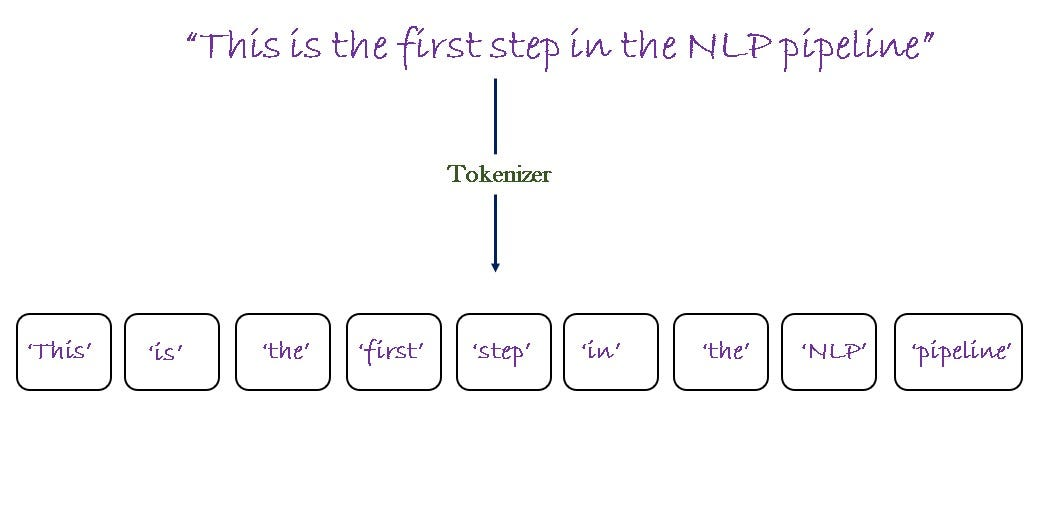
\includegraphics[width=0.99\textwidth]{assets/tokenizer.jpg}
  \caption{Tokenizzazione di una domanda in linguaggio naturale. Il tokenizer segmenta il testo in token. A ciascun token è associato un
    identificativo intero $i_k$ nel vocabolario del modello. La segmentazione mostrata è a scopo illustrativo:
    quella effettiva dipende dal tokenizer del modello considerato.}
  \label{fig:tokenizzazione}
\end{figure}

% ---------------------------------------------------------------------------
% Generazione auto-regressiva
% ---------------------------------------------------------------------------
In fase di generazione, i LLM operano in modo \emph{auto-regressivo}. Data una sequenza di token $x_1, \dots, x_t$, il modello calcola una distribuzione di probabilità sull'intero vocabolario per il token successivo, $P(x_{t+1} \mid x_1, \dots, x_t)$; da questa distribuzione viene scelto un token, il più probabile oppure uno campionato secondo la strategia di \emph{decoding} adottata, che viene accodato alla sequenza e diventa a sua volta parte del contesto per il passo seguente. Il procedimento si ripete un token alla volta, finché il modello non produce un token speciale di fine sequenza o non raggiunge un limite di lunghezza prefissato. La probabilità di un'intera sequenza si scompone quindi nel prodotto delle probabilità di ciascun token, condizionate ai token che lo precedono:
\begin{equation}
  P(x_1, \dots, x_T) = \prod_{t=1}^{T} P(x_t \mid x_1, \dots, x_{t-1}).
  \label{eq:autoregressivo}
\end{equation}
Nell'architettura Transformer questo vincolo è imposto da una \emph{maschera causale} applicata alla self-attention, che impedisce a ciascun token di considerare quelli che lo seguono. Per questo motivo i LLM generativi adottano in genere la variante \emph{decoder-only} dell'architettura, a differenza di modelli come BERT, che osservano l'intera sequenza in entrambe le direzioni e non sono pensati per generare testo. La maschera causale spiega anche perché addestramento e generazione abbiano costi così diversi: in addestramento, la sequenza è nota per intero e il modello può calcolare in parallelo le previsioni per tutte le posizioni; in generazione, invece, ogni token dipende da quelli prodotti in precedenza, e il processo è intrinsecamente sequenziale. Ne derivano due conseguenze rilevanti per questo lavoro. La prima riguarda i tempi di risposta, che crescono con la lunghezza del testo generato oltre che con quella del contesto fornito. La seconda riguarda l'affidabilità: il modello non produce la risposta nel suo insieme né rivede quanto ha già scritto, ma sceglie a ogni passo una continuazione plausibile del testo; un token errato entra nel contesto e condiziona tutti i successivi, e il campionamento introduce la componente stocastica richiamata nella Sezione~\ref{sec:problema}.

% ---------------------------------------------------------------------------
% Le tre fasi dell'addestramento
% ---------------------------------------------------------------------------
L'addestramento di un LLM avviene tipicamente in tre fasi successive, illustrate nella Figura~\ref{fig:llm-training}. Nella prima, il \emph{pre-training}, il modello
viene esposto a un corpus testuale di dimensioni enormi --- miliardi o migliaia di miliardi di token raccolti dal web, da libri, da codice sorgente --- con il solo obiettivo di predire il token successivo. Questa fase, auto-supervisionata e quindi priva di etichette fornite da esseri umani, fa emergere la competenza linguistica e una parte significativa della conoscenza fattuale del modello, codificata implicitamente nei suoi parametri \cite{zhao2023survey}.
Un modello che ha completato solo questa fase, tuttavia, non è ancora un assistente conversazionale: è un sistema di completamento testuale, che tende a proseguire il prompt ricevuto piuttosto che a rispondere a una domanda. La seconda fase, l'\emph{instruction-tuning}, affina il modello pre-addestrato in modo supervisionato su coppie istruzione-risposta scritte da esseri umani, insegnandogli a seguire le istruzioni ricevute e a rispondere nella forma attesa.

La terza fase, l'\emph{allineamento}, adatta ulteriormente il comportamento del modello alle preferenze umane, tipicamente tramite \emph{reinforcement learning from human feedback} (RLHF). Come mostra la parte inferiore della Figura~\ref{fig:llm-training}, questa fase si articola in due passaggi: prima si addestra un modello di ricompensa (\emph{reward model}) su confronti tra risposte alternative, ordinate per qualità da annotatori umani; poi si aggiorna iterativamente il modello linguistico con tecniche di apprendimento per rinforzo, usando come segnale la ricompensa stimata da quel modello. Ouyang et al. \cite{ouyang2022instructgpt}, nel lavoro che ha introdotto InstructGPT, mostrano che le ultime due fasi contano non meno della scala del modello nel renderlo utile e sicuro dal punto di vista comportamentale: un modello InstructGPT da 1,3 miliardi di parametri, sottoposto a instruction-tuning e RLHF, viene preferito dai valutatori umani a un modello GPT-3 da 175 miliardi di parametri privo di questo affinamento.

Sono quindi la seconda e la terza fase a rendere un LLM capace di rispondere in modo pertinente nella forma a una domanda posta in linguaggio naturale. Il modello resta però, come discusso nella Sezione~\ref{sec:problema}, incapace di garantire che il contenuto della risposta sia corretto o aggiornato. Né l'instruction-tuning né l'allineamento affrontano questo limite, perché esso riguarda la conoscenza codificata nei parametri e non il comportamento del modello: la conoscenza fattuale si forma quasi interamente nel pre-training, mentre le fasi successive modificano il comportamento del modello senza aggiungere, se non marginalmente, nuova conoscenza.

\begin{figure}[H]
  \centering
  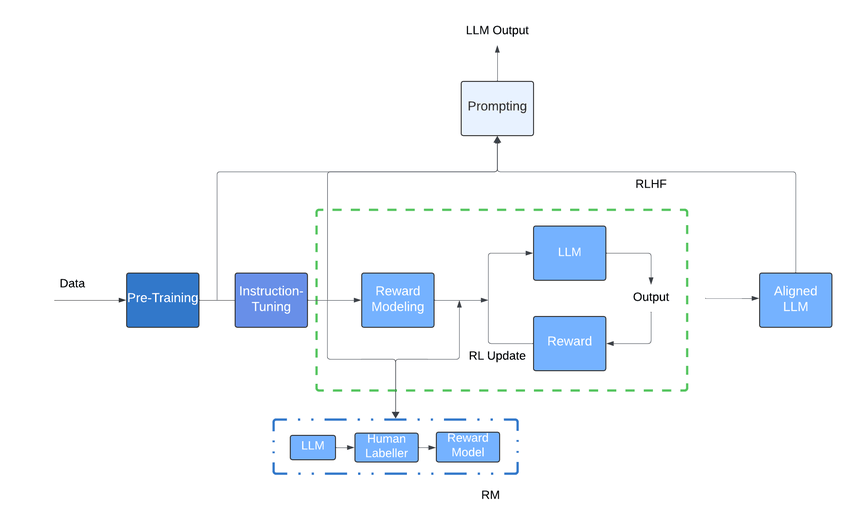
\includegraphics[width=0.9\textwidth]{assets/A-basic-flow-diagram-depicting-various-stages-of-LLMs-from-pre-training-to.png}
  \caption{Le fasi che portano dai dati grezzi a un LLM allineato e utilizzabile tramite prompting: pre-training,
    instruction-tuning e, infine, l'allineamento tramite \emph{reward modeling} (RM, in basso: un modello di
    ricompensa addestrato su confronti prodotti da annotatori umani) e \emph{reinforcement learning from human
    feedback} (RLHF, al centro: un ciclo iterativo che aggiorna l'LLM in base al segnale del modello di ricompensa).}
  \label{fig:llm-training}
\end{figure}

% ---------------------------------------------------------------------------
% Leggi di scala
% ---------------------------------------------------------------------------
Un altro aspetto, rilevante per la scelta dei modelli discussa nella sezione seguente, è il legame tra le dimensioni di un modello e la qualità delle sue previsioni. Kaplan et al. \cite{kaplan2020scaling} hanno misurato sperimentalmente come varia l'errore di predizione di un modello linguistico, cioè quanto spesso e quanto nettamente il modello sbaglia nel prevedere il token successivo, al variare di tre fattori: il numero di parametri del modello, la quantità di dati usati per addestrarlo e la potenza di calcolo complessivamente impiegata. Il risultato è una relazione sorprendentemente regolare, detta \emph{legge di scala} (\emph{scaling law}): finché gli altri due fattori non fanno da collo di bottiglia, l'errore diminuisce secondo una legge di potenza al crescere di ciascun fattore. In termini intuitivi, moltiplicare un fattore per una stessa quantità produce sempre lo stesso miglioramento in termini relativi. Secondo le stime degli autori, per esempio, raddoppiare il numero di parametri riduce l'errore di circa il 5\%, sia che si passi da 10 a 20 milioni di parametri, sia che si passi da 500 milioni a un miliardo. La Figura~\ref{fig:scaling} mostra questo andamento: su assi in scala logaritmica, le tre relazioni appaiono come rette discendenti.

Ne derivano due conseguenze. La prima è che un modello più grande, a parità di architettura e di dati di addestramento, è in genere più capace: è questa relazione, osservata ancor prima della diffusione dei moderni LLM conversazionali, a motivare l'esistenza di famiglie di modelli disponibili in più taglie, come Qwen2.5-7B e Qwen2.5-14B discussi nella sezione seguente. La seconda è che ogni ulteriore miglioramento costa sempre di più in termini assoluti: per ridurre l'errore di un'altra frazione fissa occorre ogni volta moltiplicare le risorse, e il modello più grande richiede più memoria e più tempo di calcolo per ogni risposta generata e per il training. La scelta della taglia è quindi un compromesso tra qualità delle risposte e risorse disponibili.

\begin{figure}[H]
  \centering
  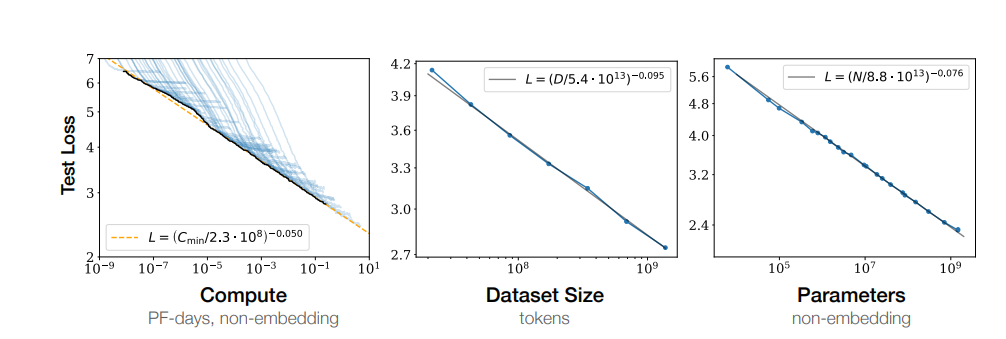
\includegraphics[width=0.9\textwidth]{assets/scale_law.png}
  \caption{Le prestazioni del modello linguistico migliorano in modo continuo man mano che aumentiamo la dimensione del modello, la dimensione del dataset e la quantità di calcolo usata per l'addestramento. Per ottenere prestazioni ottimali, tutti e tre i fattori devono essere aumentati insieme. Fonte: Kaplan et al. \cite{kaplan2020scaling}}
  \label{fig:scaling}
\end{figure}


% ---------------------------------------------------------------------------
% In-context learning
% ---------------------------------------------------------------------------
Al crescere della scala emerge anche una capacità che non corrisponde a una specifica fase di addestramento, ma che è rilevante per inquadrare il
funzionamento di un sistema RAG come quello di questo lavoro: l'\emph{in-context learning}. Brown et al.
\cite{brown2020gpt3}, presentando GPT-3, osservano che un modello linguistico sufficientemente grande può adattare il proprio comportamento a un compito nuovo semplicemente a partire da istruzioni o esempi forniti nel testo del prompt, senza alcun aggiornamento dei suoi parametri. È precisamente questo meccanismo, e non un nuovo addestramento, che un sistema RAG sfrutta quando fornisce al modello un contesto recuperato al momento della domanda (Sezione~\ref{sec:rag}): il modello non apprende un fatto nuovo in modo permanente, ma lo usa temporaneamente, limitatamente alla singola interazione in cui compare nel prompt.

% ---------------------------------------------------------------------------
% Closed-weight vs open-weight
% ---------------------------------------------------------------------------
Ai fini di questo lavoro è rilevante, infine, la distinzione tra modelli \emph{closed-weight}, accessibili solo tramite
un'interfaccia remota gestita dal fornitore e generalmente a pagamento, e modelli \emph{open-weight}, i cui parametri sono
pubblicati e possono essere eseguiti su hardware proprio. La scelta di adottare esclusivamente modelli open-weight risponde a due esigenze. La prima è il contenimento dei costi: i servizi closed-weight sono tipicamente tariffati in base al numero di token elaborati, per cui la spesa cresce con il numero di domande ricevute ed è difficile da prevedere per un servizio rivolto a un'intera università; un modello eseguito in locale comporta invece un costo legato essenzialmente all'hardware e al suo funzionamento, indipendente dal volume di utilizzo. La seconda è la tutela delle informazioni dell'ateneo: con un modello closed-weight, a ogni interrogazione la domanda dello studente e i documenti recuperati per rispondere verrebbero inviati a un fornitore esterno, mentre l'esecuzione in locale permette di non affidare a terzi documenti, contenuti del sito e informazioni proprietarie. Per questi motivi, tutti i modelli generativi considerati in
questo lavoro, descritti nella sezione seguente, sono modelli open-weight eseguibili interamente in locale.

\subsection{LLM valutati}

Il sistema sviluppato in questo lavoro è stato valutato con quattro LLM open-weight, scelti tra
quelli eseguibili sull'hardware a disposizione. Per tre di essi questo è possibile solo ricorrendo a una
quantizzazione. La \emph{quantizzazione} riduce la precisione numerica con cui sono memorizzati i pesi di un modello,
per esempio da 16 a 4 bit per peso: la memoria occupata si riduce di circa quattro volte, al prezzo di una possibile
perdita di qualità delle risposte. I tre modelli quantizzati sono serviti nella variante \emph{AWQ}
(\emph{Activation-aware Weight Quantization}), uno
schema di quantizzazione post-addestramento a 4 bit proposto da Lin et al.\ \cite{lin2024awq}. Gli autori osservano
che una piccola frazione dei pesi di un modello, quelli associati ai canali di attivazione di ampiezza maggiore,
contribuisce in modo sproporzionato all'errore di quantizzazione. AWQ individua questi pesi salienti a partire dalle
statistiche di attivazione, anziché dalla sola magnitudine dei pesi, e li protegge applicando un fattore di scala
per canale prima della quantizzazione: in questo modo la perdita di qualità si riduce drasticamente rispetto a uno
schema uniforme, senza richiedere un nuovo addestramento né una fase di backpropagation. Il quarto modello,
Llama-3.1-8B, è invece eseguito nella versione originale non quantizzata, con pesi in formato BF16 (numeri a 16 bit, la precisione con cui il modello è distribuito).

I quattro modelli confrontati sono:

\begin{itemize}
  \item \textbf{Qwen2.5-14B-Instruct-AWQ} e \textbf{Qwen2.5-7B-Instruct-AWQ}, due taglie della famiglia Qwen2.5
    sviluppata da Alibaba Cloud \cite{qwen2024technical}, che differiscono di un fattore 2 nel numero di parametri
    (14 contro 7 miliardi). Gli autori riportano un corpus di pre-training di 18 mila miliardi di token, più del
    doppio dei 7 mila miliardi della generazione precedente (Qwen2), con particolare attenzione a codice e
    matematica, e un supporto multilingue esteso a oltre 29 lingue, italiano compreso. Entrambe le varianti posseggono una finestra di contesto
    di 128k token;
  \item \textbf{Mistral-Nemo-12B-AWQ}, sviluppato congiuntamente da Mistral AI e NVIDIA
    \cite{mistralai2024nemo}, un modello da 12 miliardi di parametri con una finestra di contesto di 128k token.
    Introduce un nuovo tokenizer, Tekken, che secondo gli autori rappresenta il testo con circa il 30\% di token in
    meno rispetto al tokenizer dei precedenti modelli Mistral su codice sorgente e su diverse lingue europee, tra
    cui l'italiano, e risulta più efficiente del tokenizer di Llama~3 per circa l'85\% delle lingue. Il modello è
    stato inoltre addestrato con \emph{quantization awareness}, una procedura pensata per consentire l'inferenza in
    FP8, cioè con pesi a 8 bit;
  \item \textbf{Meta-Llama-3.1-8B-Instruct}, appartenente alla famiglia Llama~3 di Meta \cite{grattafiori2024llama3},
    composta da tre taglie dense (8, 70 e 405 miliardi di parametri) addestrate su oltre 15 mila miliardi di token,
    con una finestra di contesto di 128k token. Gli autori dichiarano un supporto ufficiale per otto lingue,
    italiano compreso, e un addestramento specifico per l'uso di strumenti esterni (\emph{tool calling}), una
    capacità agentica non rilevante per l'uso puramente conversazionale che ne fa questo sistema.
\end{itemize}

Tutti e quattro i modelli condividono la stessa architettura di fondo, il Transformer decoder-only auto-regressivo, e differiscono principalmente per numero di parametri, dati e
procedura di addestramento e tokenizer, oltre che per il formato dei pesi: Llama-3.1-8B è l'unico eseguito senza
quantizzazione, e di questa differenza occorre tenere conto nell'interpretare il confronto, perché una parte del
divario di qualità o di latenza rispetto agli altri modelli può dipendere dal formato più che dal modello in sé.
La Tabella~\ref{tab:llm_comparison} ne riassume le caratteristiche principali, mentre il confronto sistematico in termini di qualità della risposta generata, latenza e comportamento sulle diverse
categorie del dataset di test è presentato nel Capitolo~\ref{cap:validazione}.

\begin{table}[H]
    \centering
    \footnotesize
    \setlength{\tabcolsep}{4pt}
    \renewcommand{\arraystretch}{1.35}
    \begin{tabularx}{\textwidth}{@{} L{3.4cm} C{1.2cm} C{1.6cm} C{1.4cm} C{1.4cm} >{\raggedright\arraybackslash}X @{}}
        \toprule
        \textbf{Modello} & \textbf{Param.} & \textbf{Contesto} & \textbf{Formato} & \textbf{VRAM (pesi)} & \textbf{Caratteristiche principali} \\
        \midrule
        \textbf{Qwen2.5-14B-Instruct-AWQ}
            & 14,7 mld
            & 128k
            & AWQ 4 bit
            & $\sim$9--10 GB
            & Pre-training su 18 mila miliardi di token; oltre 29 lingue, italiano compreso. \\
        \midrule
        \textbf{Qwen2.5-7B-Instruct-AWQ}
            & 7,6 mld
            & 128k
            & AWQ 4 bit
            & $\sim$5--6 GB
            & Stessa famiglia del 14B con circa metà dei parametri: minore latenza e occupazione di memoria. \\
        \midrule
        \textbf{Mistral-Nemo-12B-AWQ}
            & 12,2 mld
            & 128k
            & AWQ 4 bit
            & $\sim$8--9 GB
            & Tokenizer Tekken, più compatto sull'italiano rispetto ai precedenti tokenizer Mistral. \\
        \midrule
        \textbf{Meta-Llama-3.1-8B-Instruct}
            & 8,0 mld
            & 128k
            & BF16 \newline
            & $\sim$16 GB
            & Pre-training su oltre 15 mila miliardi di token; otto lingue supportate, italiano compreso. \\
        \bottomrule
    \end{tabularx}
    \caption{Caratteristiche dei quattro modelli generativi valutati.}
    \label{tab:llm_comparison}
\end{table}


\section{RAG (Retrieval-Augmented Generation)} \label{sec:rag}

Il \emph{Retrieval-Augmented Generation} è il paradigma che Lewis et al. \cite{lewis2020retrieval} propongono per superare i due limiti discussi nella Sezione~\ref{sec:problema}: invece di affidarsi esclusivamente alla conoscenza codificata nei parametri del modello, il sistema recupera prima, da una base documentale esterna e aggiornabile, i frammenti (in inglese \emph{chunk}) di testo più pertinenti alla domanda ricevuta, e li fornisce al modello linguistico come contesto su cui basare la risposta. Il principio di fondo è separare nettamente \emph{cosa il sistema sa}, cioè l'insieme dei documenti indicizzati, che può essere aggiornato in qualunque momento senza bisogno di un nuovo addestramento, da \emph{come il sistema si esprime}, compito che resta demandato interamente al modello linguistico. Gao et al. \cite{gao2023ragsurvey}, nella loro rassegna sul tema, inquadrano questo principio come la risposta più diretta proprio ai limiti di conoscenza statica e di verificabilità discussi in precedenza: un'affermazione generata dal modello può essere ricondotta a un frammento di testo specifico, citabile e verificabile, invece che
derivare implicitamente e in modo opaco dai suoi parametri. La figura \ref{fig:rag-pipeline} mostra quella che è una pipeline generica di un sistema RAG.

\begin{figure}[H]
  \centering
  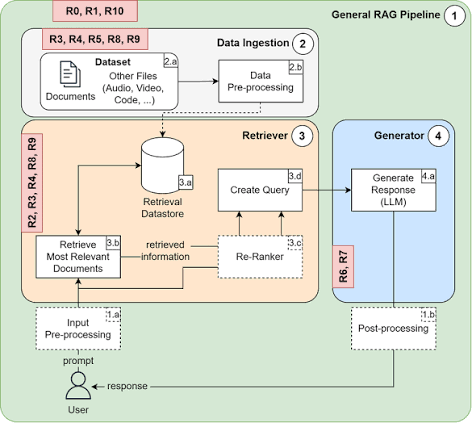
\includegraphics[width=0.6\textwidth]{assets/rag_pipeline.png}
  \caption{Schema generale di una pipeline RAG (1). Nella fase di \emph{data ingestion} (2), i documenti
  e gli altri file della collezione (2.a) vengono pre-elaborati (2.b) e indicizzati in un archivio per il
  recupero (3.a). Al momento della domanda, il prompt dell'utente viene eventualmente pre-elaborato (1.a) e
  passato al \emph{retriever} (3), che recupera i documenti più pertinenti (3.b), li riordina facoltativamente
  tramite un \emph{re-ranker} (3.c) e costruisce la richiesta da inviare al modello (3.d). Il
  \emph{generator} (4) produce la risposta tramite un LLM (4.a), che può essere post-elaborata (1.b) prima di
  essere restituita all'utente. I riquadri tratteggiati indicano componenti opzionali.}
  \label{fig:rag-pipeline}
\end{figure}

\subsection{Embedding e ricerca per similarità}\label{subsec:embedding}

Il primo problema che un sistema RAG deve risolvere è, dato un testo, come rappresentarlo in una forma che permetta
di confrontarne il significato con quello di una domanda. La soluzione standard è l'\emph{embedding}: una rete neurale
proietta ogni porzione di testo (un documento, o più spesso un suo frammento) in un vettore di numeri reali di
dimensione fissa, costruito in modo che frammenti dal significato simile vengano proiettati in punti vicini dello
spazio vettoriale. La vicinanza tra due vettori $\mathbf{u}$ e $\mathbf{v}$ si misura tipicamente con la
\emph{similarità coseno}, ovvero il coseno dell'angolo compreso tra i due vettori:
\begin{equation}
  \cos(\mathbf{u}, \mathbf{v}) = \frac{\mathbf{u} \cdot \mathbf{v}}{\lVert \mathbf{u} \rVert \, \lVert \mathbf{v} \rVert},
  \label{eq:coseno}
\end{equation}
che vale 1 per vettori con la stessa direzione e diminuisce man mano che le loro direzioni divergono.

Il punto di partenza per costruire modelli di embedding è in genere Bidirectional Encoder Representations
from Transformers (\emph{BERT}), proposto da Devlin et al.\ \cite{devlin2019bert}. A differenza dei LLM generativi descritti in precedenza, BERT utilizza solo la parte \emph{encoder} del Transformer: ogni token osserva
l'intera sequenza in entrambe le direzioni, e il modello produce per ciascun token un vettore che ne rappresenta il
significato nel contesto, senza generare testo. BERT viene pre-addestrato su grandi quantità di testo a ricostruire
parole mascherate casualmente all'interno delle frasi, e poi specializzato tramite \emph{fine-tuning} su compiti di
comprensione del linguaggio: la classificazione di un testo (per esempio l'analisi del sentiment), il riconoscimento
di entità nominate come persone e luoghi, l'individuazione della risposta a una domanda all'interno di un passaggio
dato, e la classificazione di coppie di frasi, per esempio per stabilire se due frasi sono parafrasi l'una dell'altra.

Nessuno di questi compiti, tuttavia, richiede di produrre un singolo vettore che rappresenti un'intera frase, e BERT
non è addestrato a farlo. Per confrontare due testi, BERT li riceve concatenati in un'unica sequenza e restituisce un
punteggio per la coppia, secondo un'architettura detta \emph{cross-encoder}. Reimers e Gurevych \cite{reimers2019sbert}
osservano che questo approccio è impraticabile per il recupero: ogni coppia richiede un passaggio completo attraverso
la rete, e trovare la coppia più simile in una collezione di 10.000 frasi richiede circa 50 milioni di passaggi, pari a
circa 65 ore di calcolo. D'altra parte, ricavare un vettore per ciascuna frase da BERT così com'è, per esempio facendo
la media dei vettori dei suoi token, produce embedding di bassa qualità.

La loro soluzione, Sentence-BERT (SBERT), affina BERT proprio per produrre embedding di frase confrontabili tramite la
similarità coseno. Durante l'addestramento, i due testi di ogni coppia non vengono concatenati, ma attraversano
separatamente la stessa rete, con gli stessi pesi; i due vettori risultanti vengono confrontati, e l'errore commesso
nel valutare la relazione tra i due testi (per esempio, se si tratta di parafrasi) viene usato per aggiornare i pesi.
Questa configurazione è detta \emph{siamese}, perché equivale a due copie gemelle della stessa rete. La condivisione dei
pesi garantisce che entrambi i testi vengano trasformati dalla stessa funzione, e quindi proiettati nello stesso
spazio, mentre l'addestramento fa sì che in questo spazio la similarità coseno rifletta la somiglianza di significato.
Una volta addestrata, la rete può calcolare l'embedding di ogni frammento una sola volta e indipendentemente dagli altri,
e il confronto con una domanda si riduce a una similarità coseno tra vettori già pronti: il tempo necessario a trovare
la coppia più simile tra 10.000 frasi scende così da circa 65 ore a circa 5 secondi.

Sentence-BERT è pensato per misurare la somiglianza tra frasi; nel recupero, invece, occorre confrontare una domanda
breve con passaggi di testo più lunghi che ne contengono la risposta. Karpukhin et al.\ \cite{karpukhin2020dpr}
applicano lo stesso principio a questo compito con il \emph{Dense Passage Retriever} (DPR), composto da due encoder
basati su BERT, uno per le domande e uno per i passaggi, addestrati su coppie domanda-passaggio in modo che l'embedding
di una domanda risulti vicino a quello del passaggio che contiene la risposta. Gli autori mostrano come DPR superi nettamente i metodi lessicali classici come BM25, che assegna un punteggio a ciascun documento in base alle parole che ha in
comune con la domanda, pesate secondo la loro frequenza nel documento e la loro rarità nella collezione.

Il vantaggio deriva dal fatto che un retriever basato su embedding confronta significati e non parole: una domanda come
``quando si paga la seconda rata?'' può essere associata a un passaggio che parla di ``scadenza del secondo versamento'',
pur avendo con esso quasi nessuna parola in comune. Per questo i retriever basati su embedding vengono detti
\emph{densi}, in contrapposizione alle rappresentazioni \emph{sparse} dei metodi lessicali come BM25, che descrivono un
testo con un vettore grande quanto l'intero vocabolario e composto quasi interamente da zeri. I metodi lessicali
restano comunque competitivi quando conta la corrispondenza esatta di un termine, come nel caso di codici o nomi propri.

Una domanda e un documento vengono quindi confrontati non piu sulla
base delle parole esatte che condividono, ma sulla distanza tra i rispettivi vettori nello spazio
degli embedding, calcolato in modo efficiente anche su milioni di candidati tramite strutture
dati specializzate (indici vettoriali) mantenute da un database vettoriale dedicato.

Un confronto esaustivo di un vettore query con ogni singolo vettore indicizzato (ricerca
esatta) diventa proibitivo già a poche centinaia di migliaia di frammenti, ben al di sotto della  scala di molti corpora documentali reali. I database vettoriali si affidano a una ricerca approssimata del vicino piu prossimo, che rinuncia alla garanzia di trovare sempre il risultato esatto in cambio di un tempo di
ricerca molto piu basso. Malkov e Yashunin \cite{malkov2018hnsw} propongono uno degli schemi più diffusi a
questo scopo, Hierarchical Navigable Small World (HNSW): un grafo multilivello in cui ogni
nodo rappresenta un vettore indicizzato, organizzato in strati via via piu densi, in cui la ricerca parte dallo strato piu rado (pochi nodi, collegamenti a lungo raggio) e scende progressivamente verso strati piu fitti, restringendo il raggio di ricerca a ogni passo; un meccanismo che ottiene un tempo di ricerca che cresce in modo logaritmico con il numero $N$ di vettori
indicizzati, $O(\log N)$, invece che linearmente, $O(N)$, come nella ricerca esatta.

\subsection{Ricerca ibrida e fusione dei risultati}

La ricerca per sola similarità vettoriale (\emph{dense retrieval}), tuttavia, ha un punto debole noto: tende a
performare peggio dei metodi lessicali classici (in particolare \emph{BM25} \cite{robertson2009bm25}) proprio sui termini rari o molto specifici: un codice di corso, una sigla normativa, un nome
proprio, che un embedding generico fatica a distinguere ma che un confronto esatto di parole individua senza
ambiguità. La letteratura piu recente raccomanda perciò l'adozione della \emph{ricerca ibrida} (\emph{hybrid search}): eseguire in parallelo una ricerca densa e una ricerca lessicale sparsa,
e fonderne i risultati in un'unica classifica. Una delle tecniche di fusione più diffuse a questo scopo,  è la \emph{Reciprocal Rank Fusion} (RRF), proposta da Cormack et al. \cite{cormack2009rrf}: per ogni documento si guarda non il punteggio ottenuto nelle due ricerche, ma solo la sua \emph{posizione} in ciascuna classifica e si sommano gli inversi di queste posizioni per ottenere un punteggio finale. Un documento che compare ai primi posti in entrambe le classifiche ottiene così un punteggio alto, uno che compare in alto in una sola delle due un punteggio intermedio. Il vantaggio pratico di questo meccanismo è che permette di fondere le due classifiche senza dover rendere confrontabili i punteggi originali delle due ricerche, cosa altrimenti problematica, perché il punteggio di una ricerca densa e quello di una ricerca lessicale sono calcolati in modo diverso e non sono direttamente comparabili tra loro.
\subsection{Reranking}

Il risultato della ricerca ibrida è però, tipicamente, solo una prima scrematura. Per restare efficienti su un
indice di grandi dimensioni, entrambe le sue componenti valutano ciascun frammento senza che un modello lo legga
mai insieme alla domanda. BM25 si limita a contare le parole in comune; nella componente densa, l'embedding di
ciascun frammento viene calcolato una volta per tutte, in fase di indicizzazione e quindi prima ancora di conoscere
la domanda, e al momento della ricerca viene soltanto confrontato con l'embedding della domanda tramite la
similarità coseno (Sottosezione~\ref{subsec:embedding}). Il vettore di un frammento deve perciò riassumerne l'intero
contenuto senza sapere quale aspetto interesserà a chi interroga il sistema: un frammento sulle tasse universitarie
è rappresentato sempre dallo stesso vettore, sia che la domanda riguardi la scadenza della seconda rata, sia che
riguardi l'importo previsto per una specifica fascia di reddito. Questa compressione comporta inevitabilmente una
perdita di dettaglio, e un frammento solo genericamente pertinente può finire in cima ai risultati davanti a quello
che contiene davvero la risposta. Un secondo stadio, il \emph{reranking}, corregge questo limite impiegando un
\emph{cross-encoder}: un modello che riceve domanda e documento candidato concatenati in un unico input e ne stima
direttamente la pertinenza reciproca, a un costo computazionale più alto ma applicato solo al pool già ristretto dei
migliori candidati della prima fase. Nogueira e Cho \cite{nogueira2019bert} sono tra i primi a mostrare, adattando
BERT a questo compito, che un cross-encoder di questo tipo migliora in modo sostanziale la qualità del ranking finale
rispetto alla sola similarità vettoriale.

Il cross-encoder rappresenta un estremo: domanda e documento vengono elaborati insieme, e ogni token dell'una
può essere messo in relazione con ogni token dell'altro in tutti gli strati della rete, al prezzo di dover
ripetere l'intero calcolo per ogni coppia. Esistono però soluzioni intermedie, che ottengono un confronto più dettagliato di
quello tra due singoli vettori senza sostenere il costo di un cross-encoder. Khattab e Zaharia \cite{khattab2020colbert} propongono
con ColBERT un'alternativa intermedia, la \emph{late interaction}: invece di comprimere ogni testo in un unico
vettore, ogni token di domanda e documento mantiene il proprio embedding, e la similarità complessiva si ottiene
aggregando le similarità massime tra i singoli token delle due sequenze --- un calcolo più ricco della sola
similarità tra due vettori aggregati, ma più leggero di un cross-encoder pieno, perché gli embedding dei documenti
possono comunque essere pre-calcolati e indicizzati in anticipo, mentre un cross-encoder richiede di rielaborare
congiuntamente domanda e documento a ogni confronto.
\subsection{Trasformazione della query}

Finora si è assunto implicitamente che la domanda usata per il recupero sia esattamente il testo digitato
dall'utente. Questo non è sempre il caso migliore: una domanda formulata in modo colloquiale o ellittico (che, ad esempio, fa
riferimento allo scambio precedente in una conversazione) può essere lessicalmente distante dal testo
del documento che contiene effettivamente la risposta, anche quando quel documento è topicamente pertinente. La
letteratura ha esplorato diverse strategie per colmare questa distanza riscrivendo la domanda prima di usarla per il
recupero, invece di cambiare il modo in cui i documenti vengono rappresentati. Gao et al. \cite{gao2022hyde}, con
HyDE (\emph{Hypothetical Document Embeddings}), propongono di chiedere a un LLM di generare un documento ipotetico
che risponderebbe alla domanda --- un testo che può contenere imprecisioni o essere parzialmente inventato --- e di
usare l'embedding di \emph{questo} documento, anziché quello della domanda originale, per la ricerca per similarità:
un documento ipotetico, per quanto impreciso nei dettagli, tende a essere lessicalmente e stilisticamente più vicino
ai documenti reali pertinenti di quanto non lo sia la domanda originale, spesso formulata in modo molto più
sintetico.

Un problema distinto, riguarda le domande che esprimono più di una richiesta
informativa: un singolo
passaggio di recupero sulla domanda combinata rischia di restituire chunk pertinenti a una sola delle due richieste,
perché il reranking valuta ogni candidato contro l'intera domanda invece che contro le sue parti. Ammann et al.
\cite{ammann2025decomposition} affrontano esplicitamente questo caso con la \emph{decomposizione della domanda}: un
LLM scompone la domanda originale in una o più sotto-domande autonome, il recupero viene eseguito separatamente per
ciascuna, e i risultati vengono fusi e riordinati con un cross-encoder standard --- un approccio che gli autori
mostrano migliorare il recupero su benchmark di question answering multi-hop (cioè un insieme standard di domande con risposte note usato per confrontare sistemi diversi) in cui la risposta richiede di combinare informazioni contenute in documenti diversi, senza richiedere alcun addestramento
aggiuntivo o indicizzazione specializzata.
\subsection{Chunking e fusione gerarchica}

Un ultimo problema, trasversale a tutti gli stadi precedenti, è quello del \emph{chunking}: un documento specie se lungo, come un regolamento o una dispensa, non può essere indicizzato come unico blocco, sia per limiti di
lunghezza degli input dei modelli di embedding sia perché un frammento troppo esteso diluisce il segnale specifico
cercato dalla domanda in mezzo a informazione non pertinente. La scelta della dimensione dei frammenti è però essa
stessa un compromesso: frammenti troppo corti rischiano di perdere il contesto necessario a renderli comprensibili
in isolamento, frammenti troppo lunghi tornano a soffrire del problema opposto.

La strategia più semplice consiste nel suddividere il testo in blocchi di dimensione fissa, eventualmente con una
sovrapposizione tra blocchi consecutivi per non spezzare un'informazione a cavallo del confine. Questo approccio tuttavia ignora la
struttura logica del documento: un paragrafo coerente può essere tagliato a metà solo perché il conteggio dei token ha raggiunto la soglia impostata. Un'alternativa più sensibile al contenuto è il \emph{chunking strutturale}, che rispetta i confini naturali del documento (sezioni, paragrafi, righe di una tabella) invece di tagliare a una lunghezza fissa, cedendo una parte dell'uniformità dei frammenti risultanti in cambio di un testo internamente più coerente. Nessuna delle due strategie, da sola, risolve però il problema opposto: un frammento strutturalmente coerente ma troppo corto (un singolo titolo di sezione, una riga isolata di una tabella) resta comunque privo del contesto che lo renderebbe comprensibile se recuperato in isolamento.

Una soluzione a questo problema è la \emph{fusione gerarchica} dei frammenti. In fase di
indicizzazione ogni documento viene diviso in frammenti piccoli, che sono quelli effettivamente
indicizzati e confrontati con la domanda, ma si conserva anche il legame di ciascun frammento con
la sezione del documento a cui appartiene. Al momento del recupero, se tra i frammenti selezionati
ne compaiono abbastanza appartenenti alla stessa sezione, questi vengono sostituiti dalla sezione
intera: il recupero conserva così la precisione dei frammenti piccoli, mentre il modello riceve un
contesto ampio e coerente.

\subsection{Posizione del contesto nel prompt}

Un'ultima scelta, a valle di tutte quelle discusse finora, riguarda come assemblare nel prompt i frammenti
recuperati, ordinati per pertinenza: semplicemente concatenarli nell'ordine restituito dal reranking non è
necessariamente innocuo. Liu et al. \cite{liu2023lostmiddle} mostrano che un LLM non utilizza un contesto lungo in
modo uniforme: l'accuratezza nel reperire un'informazione specifica è più alta quando questa si trova all'inizio o
alla fine del contesto fornito, e cala sensibilmente quando si trova nel mezzo un andamento a U che gli autori
osservano persistere anche in modelli progettati esplicitamente per finestre di contesto lunghe, e che ricorda gli
effetti di primacy e recency studiati nella memoria umana(vedere la figura: \ref{fig:u-curve}).
\begin{figure}[H]
  \centering
  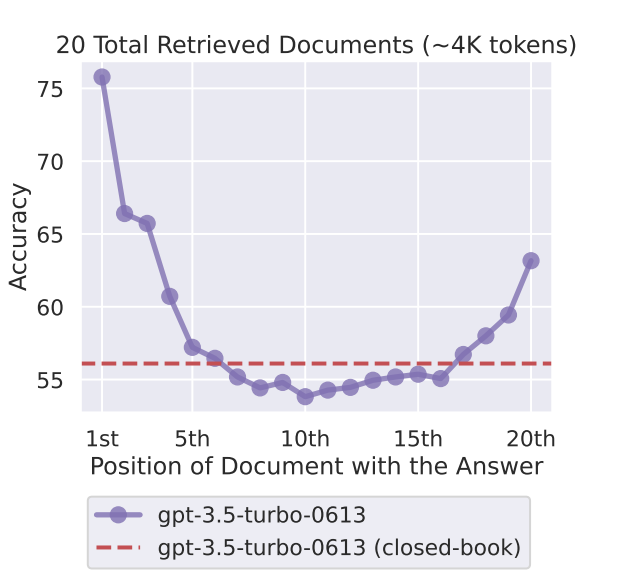
\includegraphics[width=0.5\textwidth]{assets/U-curve-diagram.png}
  \caption{La modifica della posizione delle informazioni rilevanti (in questo caso, la posizione del passaggio che risponde a una domanda in input) all'interno del contesto di input del modello linguistico produce una curva delle prestazioni a forma di U: i modelli sono più abili nell'utilizzare le informazioni rilevanti che compaiono all'inizio o alla fine del proprio contesto di input, e le prestazioni diminuiscono in modo significativo quando i modelli devono accedere e utilizzare informazioni situate nella parte centrale del proprio contesto di input. Fonte: Liu et al. \cite{liu2023lostmiddle} }
  \label{fig:u-curve}
\end{figure}

Per un sistema che costruisce il proprio contesto
unendo più frammenti recuperati, come quello di questo lavoro, questo risultato implica che l'ordine con cui i
frammenti vengono presentati al modello non è un dettaglio ininfluente quanto potrebbe sembrare a prima vista, specie
quando il numero di frammenti recuperati si avvicina al
limite superiore per cui l'effetto è stato osservato in letteratura.

\section{Sistemi che utilizzano LLM e RAG per rispondere in maniera automatica} \label{sec:sistemi-simili}

I chatbot per l'assistenza universitaria non nascono con i LLM: le prime generazioni di questi sistemi, risalenti a
ben prima della diffusione dei Transformer, si basavano su alberi di decisione scritti a mano o su classificatori
statistici, abbinati a un insieme limitato e predefinito di risposte. Erano sistemi capaci di gestire bene le
domande più frequenti, previste in fase di progettazione, ma fragili di fronte a qualunque formulazione che si
discostasse dal copione atteso. L'arrivo di LLM in grado di comprendere una domanda espressa liberamente, combinati
con il paradigma RAG per ancorare la risposta a documenti reali invece che a un insieme fisso di risposte
prestabilite, segna il passaggio a una nuova generazione di sistemi: capaci, in linea di principio, di rispondere a
qualunque domanda per cui esista un documento pertinente nella base indicizzata, senza dover prevedere a priori ogni
possibile formulazione.

L'applicazione di LLM e RAG all'assistenza universitaria non è, a questo punto, un'idea isolata. Peyton et al.
\cite{peyton2025review}, in una rassegna recente dedicata ai chatbot universitari per il supporto agli studenti,
confrontano otto implementazioni distinte e osservano come il settore non abbia ancora sfruttato appieno il
potenziale di questi sistemi rispetto ad altri ambiti applicativi, in parte per la difficoltà di reperire e curare
dataset di dominio chiuso, specifici di un singolo ateneo, su cui valutarli in modo affidabile. È un'osservazione
che motiva direttamente la scelta di questo lavoro di costruire un dataset diagnostico dedicato
(Capitolo~\ref{cap:validazione}), invece di affidarsi a benchmark generici.

Tre sistemi recenti sono particolarmente vicini, per dominio e impostazione, a quello sviluppato in questo lavoro.
Unipa-GPT \cite{siragusa2024unipagpt}, sviluppato per l'Università di Palermo, è un assistente conversazionale in
italiano rivolto a potenziali studenti che devono scegliere un corso di laurea triennale o magistrale. Gli autori
confrontano esplicitamente un approccio RAG, che recupera il contesto da un corpus raccolto dal sito web
dell'ateneo, con un approccio di fine-tuning dello stesso modello di base: un punto di riferimento diretto, su un
dominio analogo a quello di questo progetto, per la stessa alternativa architetturale discussa nella
Sezione~\ref{sec:rag}. Marcel \cite{trienes2025marcel}, sviluppato per l'Università di Marburg, si concentra invece
sulle domande più frequenti dei futuri studenti relative all'ammissione, e affianca alla ricerca sui documenti un
retriever dedicato alle FAQ: in questo modo il personale amministrativo può orientare esplicitamente le risposte
alle domande ricorrenti, invece di affidarsi interamente all'indicizzazione automatica dei documenti originali.
Vlahek \cite{vlahek2024chatbot}, infine, descrive un prototipo di chatbot RAG per il supporto agli studenti
universitari realizzato con uno strumento \emph{low-code} (Flowise AI), invece che con una pipeline sviluppata su
misura come nei due casi precedenti. Il lavoro conferma che la combinazione di LLM e RAG per questo tipo di compito
è ormai accessibile anche senza un'implementazione interamente personalizzata, benché a scapito del controllo
puntuale su ciascuno stadio della pipeline (chunking, ricerca ibrida, reranking) discusso nella
Sezione~\ref{sec:rag}, centrale nelle scelte di questo lavoro.

Il quadro non è però limitato all'ambito universitario: sistemi LLM più RAG vengono ormai distribuiti anche in
contesti industriali, e la letteratura che ne documenta la realizzazione è complementare a quella dei sistemi
accademici, perché si concentra sui problemi di ingegnerizzazione che emergono una volta messo in uso un sistema
reale, più che sulla sola qualità delle risposte misurata su un benchmark. Barnett et al.
\cite{barnett2024sevenfailures} riportano l'esperienza di tre implementazioni RAG distinte, in ambito di ricerca,
educativo e biomedico, e ne ricavano sette punti di fallimento ricorrenti. Tra questi il \emph{missing content}, in
cui il documento necessario a rispondere non è presente nella base indicizzata, e il \emph{missed top-ranked
document}, in cui il documento pertinente esiste nell'indice ma non emerge tra i candidati restituiti dal recupero.
Gli autori osservano inoltre che la robustezza di un sistema RAG si costruisce iterativamente con l'uso reale e non
può essere interamente garantita in fase di progettazione. Bourdin et al. \cite{bourdin2025easirag} documentano un
caso concreto di questo tipo in un contesto manifatturiero: un laboratorio di test ambientali che ha realizzato un
assistente RAG per rispondere alle domande degli operatori a partire dalle procedure operative interne.

Letti insieme, i sistemi universitari descritti condividono con questo lavoro l'impostazione di fondo --- LLM più
RAG, applicato alle domande degli studenti di un singolo ateneo --- ma nessuno descrive come gestire una domanda la
cui risposta dipende dal corso di laurea dello studente, quando questa informazione non è esplicita nel testo della
domanda. Unipa-GPT e Vlahek operano su un unico corpus (rispettivamente l'intero ateneo di Palermo e un singolo
corso), dove il problema non si pone nella stessa forma; Marcel, pur limitato alle sole domande di ammissione, non
discute casi di ambiguità tra profili di studenti diversi.

È in questo spazio che si colloca il presente lavoro. Il sistema sviluppato indicizza insieme le pagine di più corsi
di laurea, le pagine generali di ateneo e i materiali didattici: la stessa domanda --- una scadenza, un requisito,
un referente --- può quindi avere risposte diverse a seconda del corso. Per questo il sistema riconosce quando una
domanda è ambigua rispetto al corso, chiede allo studente di indicarlo, e usa poi il corso noto per privilegiare i
documenti pertinenti, senza escludere quelli degli altri corsi o di ateneo. La soluzione adottata è descritta nel
Capitolo~\ref{cap:architettura} e valutata nel Capitolo~\ref{cap:validazione}.



\chapter{Architettura e sviluppo del sistema}\label{cap:architettura}

Il Capitolo~\ref{cap:stato_arte} ha presentato il paradigma RAG e le tecniche che la letteratura propone per
ciascuno dei suoi stadi. Questo capitolo descrive come quelle tecniche sono state selezionate, adattate e combinate
nel sistema sviluppato, con un livello di dettaglio sufficiente a comprenderne il funzionamento senza dover
ricorrere al codice sorgente.

Le scelte descritte nel seguito discendono in larga parte da quattro vincoli di progetto. Il primo è la
\textbf{riservatezza}: l'intero sistema, dai modelli linguistici al database vettoriale, viene eseguito in locale,
senza alcuna chiamata a servizi cloud di terze parti. Il secondo è l'\textbf{hardware disponibile}: il sistema è stato
sviluppato e valutato sulle risorse messe a disposizione per il progetto, due GPU da 16~GB ciascuna, una dedicata
al modello linguistico e l'altra ai modelli di embedding e di reranking; durante l'indicizzazione se ne aggiunge
temporaneamente una terza, per il modello multimodale che descrive le immagini dei documenti. Quest'ultima è
una conseguenza della scelta di generare le risposte con un modello solo testuale:
con un modello multimodale in grado di svolgere entrambi i compiti, non sarebbe più necessaria. Questa configurazione esclude i modelli
linguistici di dimensioni maggiori e ha guidato il dimensionamento di ogni componente; non è però un requisito del
sistema, che con risorse diverse potrebbe adottare modelli più grandi senza modifiche alla sua architettura. Il terzo è la \textbf{precisione fattuale}: in un dominio
fatto di scadenze, importi e requisiti, una risposta fluida ma con una data sbagliata è peggiore di una risposta che
ammette di non conoscere l'informazione, e questo principio orienta tanto il recupero quanto la generazione. Il
quarto, infine, è la \textbf{natura del dominio}: il sistema indicizza insieme le pagine di più corsi di laurea,
le pagine generali di ateneo e i materiali didattici, documenti eterogenei per formato e struttura, e la risposta a
una stessa domanda può cambiare a seconda del corso dello studente.

\section{Panoramica dell'architettura}\label{sec:panoramica}

Il sistema si articola in due processi distinti: un processo di \emph{indicizzazione}, eseguito in anticipo e
ripetuto solo quando i documenti cambiano, che trasforma la documentazione dell'ateneo in una base di conoscenza
interrogabile; e un processo di \emph{risposta}, eseguito a ogni domanda dello studente, che interroga quella base e
costruisce la risposta. I due processi condividono un unico punto di contatto, l'archivio in cui l'indicizzazione
deposita i frammenti di testo e da cui la risposta li recupera: è questa separazione a rendere la conoscenza del
sistema aggiornabile senza intervenire sul modello linguistico, secondo il principio del RAG discusso nella
Sezione~\ref{sec:rag}. A questi due processi se ne affianca un terzo, la \emph{valutazione}, che misura la qualità
del sistema su un insieme di domande di test.

\subsection*{Componenti}

Il sistema è composto da sette componenti, rappresentati nella Figura~\ref{fig:componenti} e corrispondenti ai
moduli in cui è organizzato il codice.

\begin{figure}[H]
  \centering
  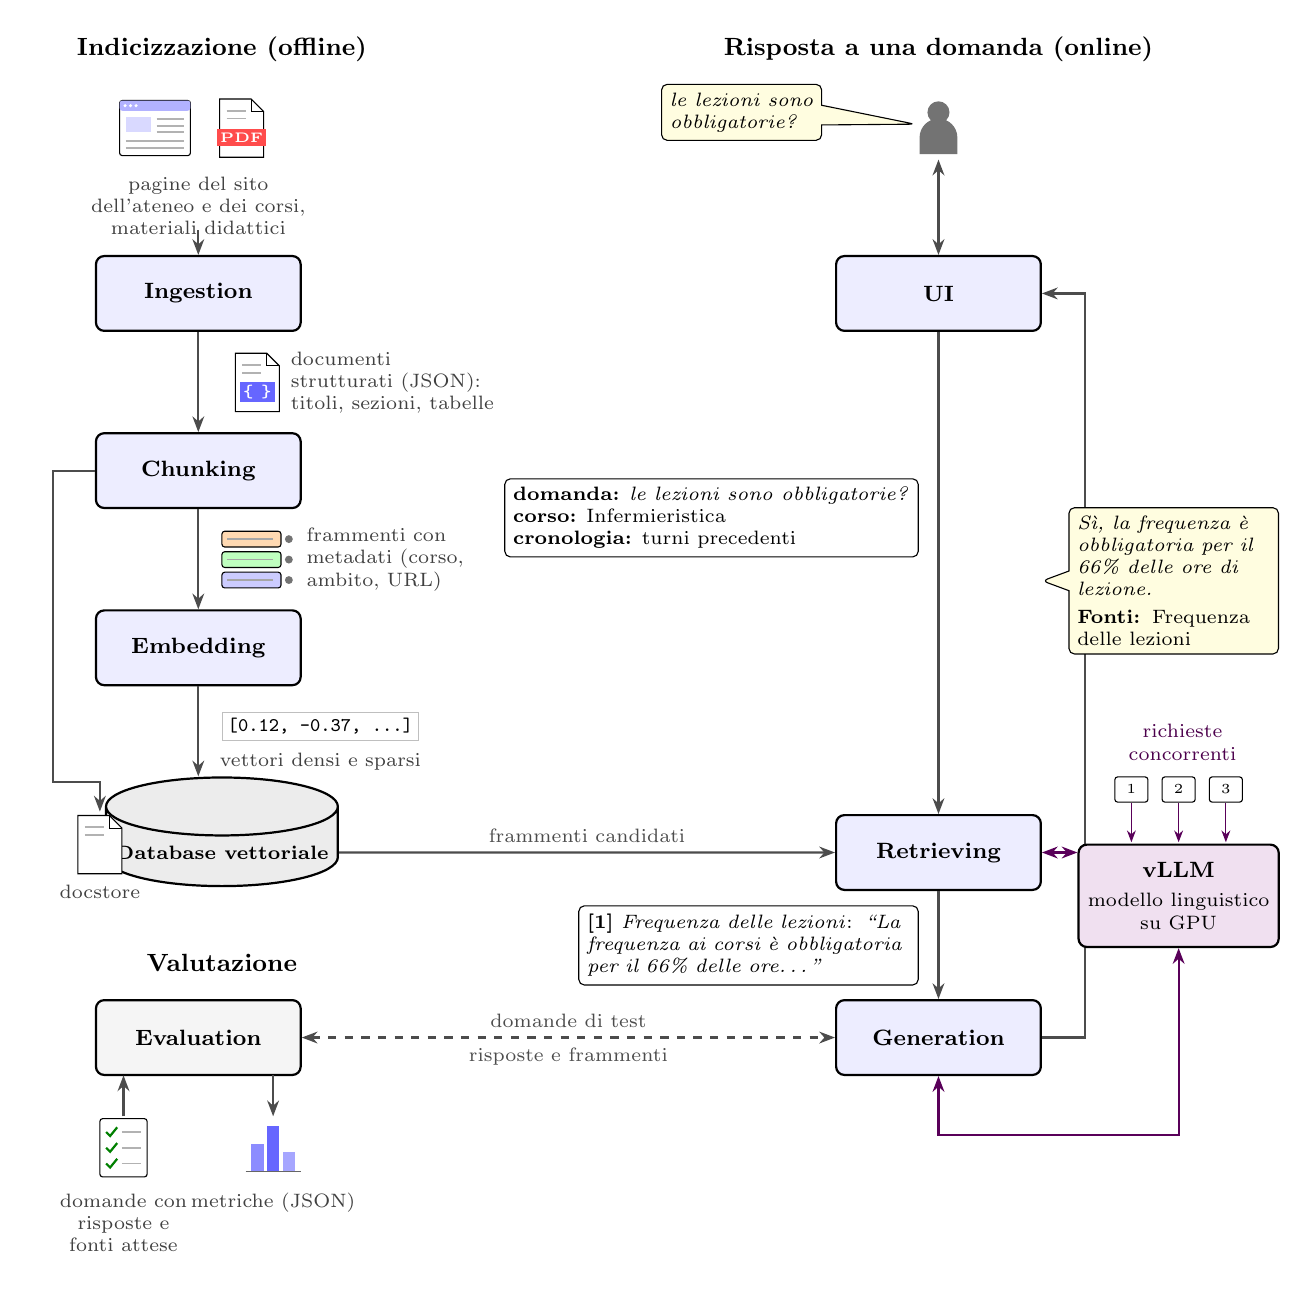
\begin{tikzpicture}[
      comp/.style={draw, thick, rounded corners=3pt, align=center, minimum width=2.6cm, minimum height=0.95cm,
                   font=\footnotesize\bfseries, fill=blue!7},
      lab/.style={font=\scriptsize, align=left, text width=2.6cm, text=black!75},
      labL/.style={lab, align=right},
      arr/.style={-{Stealth[length=2mm]}, thick, black!70},
      head/.style={font=\small\bfseries},
      bubble/.style={draw, rectangle callout, rounded corners=2pt, fill=yellow!12, font=\scriptsize\itshape,
                     align=left, inner sep=3pt},
      card/.style={draw, rounded corners=2pt, fill=white, font=\scriptsize, align=left, inner sep=3pt},
      % icona: pagina web
      webpage/.pic={
        \draw[rounded corners=1pt, fill=white] (-0.45,-0.35) rectangle (0.45,0.35);
        \fill[blue!30, rounded corners=1pt] (-0.45,0.22) rectangle (0.45,0.35);
        \foreach \x in {-0.38,-0.31,-0.24} \fill[white] (\x,0.285) circle (0.022);
        \fill[blue!15] (-0.37,-0.05) rectangle (-0.05,0.14);
        \foreach \y in {0.11,0.03,-0.05} \draw[gray!60, line width=0.7pt] (0.02,\y) -- (0.37,\y);
        \foreach \y in {-0.16,-0.25} \draw[gray!60, line width=0.7pt] (-0.37,\y) -- (0.37,\y);
      },
      % icona: documento con angolo piegato e un'etichetta
      doc/.pic={
        \draw[fill=white] (-0.28,-0.37) -- (-0.28,0.37) -- (0.12,0.37) -- (0.28,0.21) -- (0.28,-0.37) -- cycle;
        \draw (0.12,0.37) -- (0.12,0.21) -- (0.28,0.21);
        \foreach \y in {0.22,0.12} \draw[gray!60, line width=0.6pt] (-0.19,\y) -- (0.05,\y);
        \node[fill=#1, text=white, font=\tiny\bfseries, inner sep=1.2pt] at (0,-0.12) {\tikzpictext};
      },
      % icona: frammenti con metadati
      chunks/.pic={
        \foreach \y/\c in {0.26/orange!30, 0/green!25, -0.26/blue!20} {
          \draw[fill=\c, rounded corners=1pt] (-0.45,\y-0.1) rectangle (0.3,\y+0.1);
          \draw[gray!70, line width=0.5pt] (-0.38,\y) -- (0.2,\y);
          \fill[black!55] (0.4,\y) circle (0.05);
        }
      },
      % icona: studente
      student/.pic={
        \fill[black!55] (0,0.2) circle (0.14);
        \fill[black!55] (-0.24,-0.33) -- (-0.24,-0.12) arc (180:0:0.24) -- (0.24,-0.33) -- cycle;
      },
      % icona: insieme di test
      checklist/.pic={
        \draw[fill=white, rounded corners=1pt] (-0.3,-0.37) rectangle (0.3,0.37);
        \foreach \y in {0.2,0,-0.2} {
          \draw[green!50!black, line width=0.8pt] (-0.22,\y) -- (-0.17,\y-0.05) -- (-0.08,\y+0.06);
          \draw[gray!60, line width=0.6pt] (-0.02,\y) -- (0.22,\y);
        }
      },
      % icona: metriche
      bars/.pic={
        \draw[black!60] (-0.35,-0.3) -- (0.35,-0.3);
        \fill[blue!45] (-0.28,-0.3) rectangle (-0.12,0.05);
        \fill[blue!60] (-0.08,-0.3) rectangle (0.08,0.28);
        \fill[blue!35] (0.12,-0.3) rectangle (0.28,-0.05);
      },
    ]

    % ================= Indicizzazione =================
    \node[head] at (0.3,1.35) {Indicizzazione (offline)};
    \pic at (-0.55,0.35) {webpage};
    \pic[pic text=PDF] at (0.55,0.35) {doc=red!70};
    \node[lab, align=center, text width=3.4cm, anchor=north] at (0,-0.15) {pagine del sito dell'ateneo e dei corsi,
      materiali didattici};
    \node[comp] (ing) at (0,-1.75) {Ingestion};
    \node[comp] (chu) at (0,-4.0) {Chunking};
    \node[comp] (emb) at (0,-6.25) {Embedding};
    \node[cylinder, shape border rotate=90, draw, thick, aspect=0.25, minimum height=1.25cm,
          minimum width=1.5cm, fill=gray!15, font=\scriptsize\bfseries] (qd) at (0.3,-8.85) {Database vettoriale};
    \pic[pic text={\ }] at (-1.25,-8.75) {doc=white};
    \node[lab, align=center, text width=1.4cm] at (-1.25,-9.35) {docstore};

    \draw[arr] (0,-0.95) -- (ing);
    \draw[arr] (ing) -- (chu);
    \pic[pic text={\{ \}}] at (0.75,-2.88) {doc=blue!60};
    \node[lab, right] at (1.05,-2.88) {documenti strutturati (JSON): titoli, sezioni, tabelle};
    \draw[arr] (chu) -- (emb);
    \pic at (0.75,-5.13) {chunks};
    \node[lab, right] at (1.25,-5.13) {frammenti con metadati (corso, ambito, URL)};
    \draw[arr] (emb.south) -- (emb.south |- qd.north);
    \node[font=\ttfamily\scriptsize, fill=white, draw=black!25, inner sep=2pt] at (1.55,-7.25)
      {[0.12, -0.37, \dots]};
    \node[lab, right] at (0.15,-7.7) {vettori densi e sparsi};
    \draw[arr] (chu.west) -| (-1.85,-6.0) |- (-1.25,-7.95) -- (-1.25,-8.33);

    % ================= Risposta =================
    \node[head] at (9.4,1.35) {Risposta a una domanda (online)};
    \pic at (9.4,0.35) {student};
    \node[bubble, callout absolute pointer={(9.1,0.4)}] at (6.9,0.55) {le lezioni sono\\obbligatorie?};
    \node[comp] (ui) at (9.4,-1.75) {UI};
    \draw[arr, {Stealth[length=2mm]}-{Stealth[length=2mm]}] (9.4,-0.05) -- (ui);
    \node[comp] (ret) at (9.4,-8.85) {Retrieving};
    \node[comp] (gen) at (9.4,-11.2) {Generation};

    \draw[arr] (ui) -- (ret);
    \node[card, anchor=east] at (9.15,-4.6) {\textbf{domanda:} \emph{le lezioni sono obbligatorie?}\\
      \textbf{corso:} Infermieristica\\ \textbf{cronologia:} turni precedenti};

    \draw[arr] (qd.east) -- node[above, font=\scriptsize] {frammenti candidati} (ret.west);

    \draw[arr] (ret) -- (gen);
    \node[card, anchor=east, text width=4.1cm] at (9.15,-10.03) {\textbf{[1]} \emph{Frequenza delle lezioni}:
      \emph{``La frequenza ai corsi è obbligatoria per il 66\% delle ore\dots''}};

    \draw[arr] (gen.east) -- ++(0.55,0) |- (ui.east);
    \node[bubble, callout absolute pointer={(10.72,-5.4)}, anchor=west, text width=2.45cm] at (11.05,-5.4)
      {Sì, la frequenza è obbligatoria per il 66\% delle ore di lezione.\\[2pt]
       \upshape\textbf{Fonti:} Frequenza delle lezioni};

    % ================= vLLM =================
    \node[draw, thick, rounded corners=3pt, fill=violet!12, align=center, minimum width=2.0cm,
          minimum height=1.3cm, font=\footnotesize] (vllm) at (12.45,-9.4)
      {\textbf{vLLM}\\[1pt]{\scriptsize modello linguistico}\\[-1pt]{\scriptsize su GPU}};
    \foreach \x/\t in {11.85/1, 12.45/2, 13.05/3} {
      \node[draw, rounded corners=1pt, fill=white, font=\tiny, minimum width=0.42cm, minimum height=0.32cm,
            inner sep=1pt] (req\t) at (\x,-8.05) {\t};
      \draw[-{Stealth[length=1.5mm]}, violet!70!black] (req\t.south) -- (\x,-8.72);
    }
    \node[font=\scriptsize, text=violet!60!black, align=center, text width=1.9cm] at (12.5,-7.45)
      {richieste concorrenti};
    \draw[{Stealth[length=2mm]}-{Stealth[length=2mm]}, thick, violet!70!black] (ret.east) -- (ret.east -| vllm.west);
    \draw[{Stealth[length=2mm]}-{Stealth[length=2mm]}, thick, violet!70!black]
      (gen.south) -- ++(0,-0.75) -| (vllm.south);

    % ================= Valutazione =================
    \node[head] at (0.3,-10.25) {Valutazione};
    \node[comp, fill=gray!8] (eva) at (0,-11.2) {Evaluation};
    \pic at (-0.95,-12.6) {checklist};
    \node[lab, align=center, text width=2.2cm] at (-0.95,-13.55) {domande con risposte e fonti attese};
    \pic at (0.95,-12.6) {bars};
    \node[lab, align=center, text width=2.2cm] at (0.95,-13.3) {metriche (JSON)};
    \draw[arr] (-0.95,-12.2) -- (-0.95,-11.68);
    \draw[arr] (0.95,-11.68) -- (0.95,-12.2);
    \draw[arr, dashed, {Stealth[length=2mm]}-{Stealth[length=2mm]}] (eva) --
      node[above, font=\scriptsize] {domande di test} node[below, font=\scriptsize] {risposte e frammenti} (gen);
  \end{tikzpicture}
  \caption{Componenti del sistema e dati che si scambiano, seguendo una domanda di esempio. A sinistra
  l'indicizzazione trasforma pagine web e documenti in frammenti e vettori, salvati nel database vettoriale e nel docstore; a
  destra la domanda dello studente attraversa interfaccia, recupero e generazione, fino alla risposta con la fonte
  citata. In basso la valutazione sottopone alla stessa pipeline le domande di test e ne misura la qualità.
  L'Embedding opera anche al momento della domanda, per rappresentarla nello stesso spazio vettoriale dei
  frammenti. In viola le chiamate al modello linguistico, servito da vLLM: le inviano il Retrieving (analisi della
  domanda, HyDE) e la Generation; vLLM elabora insieme le richieste che arrivano contemporaneamente, anche da
  domande di studenti diversi. Per descrivere le immagini, in fase di indicizzazione l'Ingestion usa una seconda
  istanza di vLLM con un modello multimodale, attiva solo durante la conversione.}
  \label{fig:componenti}
\end{figure}

\paragraph{Ingestion.} Acquisisce i documenti e li porta in un formato strutturato comune. Le pagine web dei corsi
di laurea e di ateneo vengono scaricate da un crawler dedicato; queste e gli altri documenti (PDF, presentazioni)
vengono poi convertiti con Docling in una rappresentazione che conserva titoli, sezioni e tabelle, e corretti dalle
imprecisioni ricorrenti della conversione.

\paragraph{Chunking.} Suddivide ogni documento convertito in frammenti che rispettano la struttura delle sezioni e
associa a ciascuno i metadati necessari al recupero, tra cui il corso di laurea a cui appartiene o l'indicazione che
si tratta di una pagina di ateneo. Conserva inoltre il legame tra i frammenti e la sezione da cui provengono, usato
dalla fusione gerarchica in fase di recupero.

\paragraph{Embedding.} Calcola la rappresentazione vettoriale di ogni frammento, densa e sparsa, e la salva nel
database vettoriale insieme ai metadati; lo stesso modello calcola, al momento della domanda, la rappresentazione
della domanda stessa.

\paragraph{Retrieving.} A ogni domanda individua i frammenti pertinenti: analizza la domanda (ne ricostruisce il
senso rispetto alla conversazione, la scompone se contiene più richieste, riconosce il corso di laurea), cerca i
candidati tra le pagine di ateneo e quelle del corso, li riordina in base alla pertinenza e scarta quelli
insufficienti.

\paragraph{Generation.} Costruisce il prompt con la domanda e i frammenti recuperati, interroga il modello
linguistico e restituisce la risposta con le fonti citate. Quando il recupero non produce frammenti pertinenti, il
modello non viene interpellato per rispondere.

\paragraph{UI.} È l'interfaccia di chat con cui lo studente interagisce e il punto in cui il percorso di una domanda
viene coordinato: mantiene la cronologia della conversazione e il corso dello studente, decide quando chiedere
all'utente di indicare il corso e mostra la risposta man mano che viene generata.

\paragraph{Evaluation.} Esegue lo stesso percorso di recupero e generazione su un insieme di domande di test con
risposta nota e ne misura la qualità, separatamente per il recupero e per la risposta finale. Non fa parte del
sistema in esercizio, ma è lo strumento con cui sono state verificate le scelte descritte in questo capitolo
(Capitolo~\ref{cap:validazione}).

\medskip
\noindent La Tabella~\ref{tab:componenti} riassume, per ciascun componente, le tecnologie adottate e il momento in
cui opera;

\begin{table}[H]
  \centering
  \footnotesize
  \begin{tabularx}{\textwidth}{@{} L{2.2cm} >{\raggedright\arraybackslash}X L{3.4cm} @{}}
    \toprule
    \textbf{Componente} & \textbf{Tecnologie} & \textbf{Quando opera} \\
    \midrule
    Ingestion & crawler dedicato, Docling & indicizzazione \\
    Chunking & Docling, LlamaIndex & indicizzazione \\
    Embedding & BGE-M3, Qdrant & indicizzazione e a ogni domanda \\
    Retrieving & Qdrant, bge-reranker-v2-m3, LlamaIndex, modello linguistico & a ogni domanda \\
    Generation & modello linguistico (Qwen2.5-14B-Instruct) servito da vLLM & a ogni domanda \\
    UI & Chainlit & a ogni domanda \\
    Evaluation & RAGAS e metriche di recupero dedicate & solo in valutazione \\
    \bottomrule
  \end{tabularx}
  \caption{Componenti del sistema, tecnologie adottate e momento in cui operano.}
  \label{tab:componenti}
\end{table}


\section{Ingestione e preparazione dei dati}\label{sec:ingestione}

La qualità delle risposte di un sistema RAG è limitata dalla qualità dei frammenti che il recupero può restituire:
un'informazione persa, spezzata o deformata durante la preparazione dei documenti non può essere recuperata in
seguito, per quanto accurati siano i passi successivi. Questa sezione descrive come i documenti vengono
acquisiti, convertiti in un formato uniforme, ripuliti e suddivisi in frammenti corredati di metadati. Il percorso,
riassunto nella Figura~\ref{fig:pipeline-ingestione}, è affidato ai componenti Ingestion e Chunking
(Sezione~\ref{sec:panoramica}).

\begin{figure}[H]
  \centering
  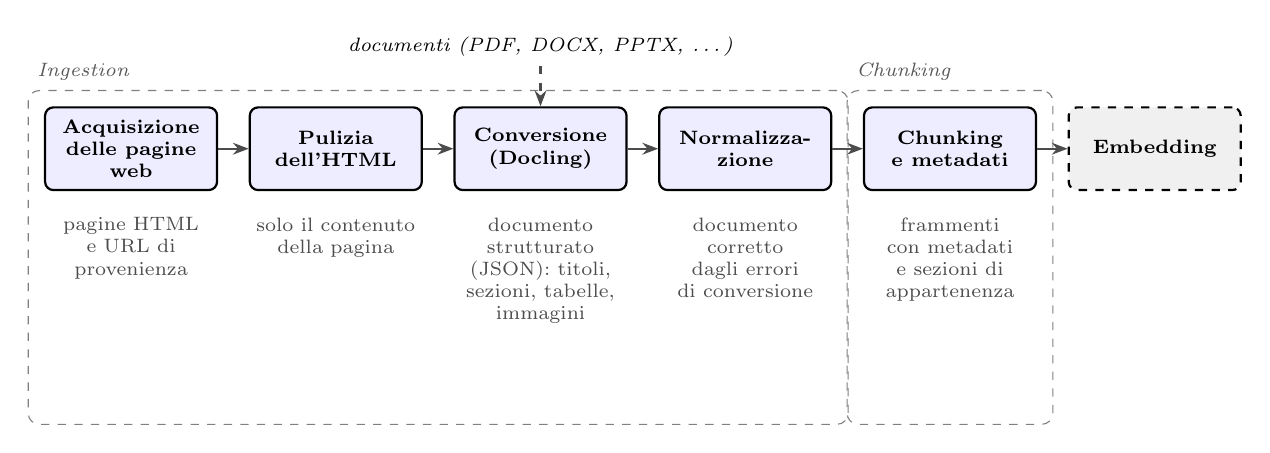
\begin{tikzpicture}[
      stage/.style={draw, thick, rounded corners=3pt, fill=blue!7, align=center, text width=1.95cm,
                   minimum height=1.05cm, font=\scriptsize\bfseries},
      res/.style={align=center, text width=2.15cm, font=\scriptsize, text=black!70, anchor=north},
      arr/.style={-{Stealth[length=2mm]}, thick, black!70},
      grp/.style={draw=gray, dashed, rounded corners=4pt, inner sep=2mm},
      grplabel/.style={font=\scriptsize\itshape, text=gray!70!black, anchor=south west},
    ]
    \node[stage] (crawl) at (0,0) {Acquisizione delle pagine web};
    \node[stage] (pre) at (2.6,0) {Pulizia dell'HTML};
    \node[stage] (conv) at (5.2,0) {Conversione (Docling)};
    \node[stage] (norm) at (7.8,0) {Normalizza\-zione};
    \node[stage] (chunk) at (10.4,0) {Chunking e metadati};
    \node[stage, fill=gray!12, dashed] (emb) at (13.0,0) {Embedding};
    \foreach \a/\b in {crawl/pre, pre/conv, conv/norm, norm/chunk, chunk/emb} \draw[arr] (\a) -- (\b);

    \node[res] at (0,-0.75) {pagine HTML e URL di provenienza};
    \node[res] at (2.6,-0.75) {solo il contenuto della pagina};
    \node[res] at (5.2,-0.75) {documento strutturato (JSON): titoli, sezioni, tabelle, immagini};
    \node[res] at (7.8,-0.75) {documento corretto dagli errori di conversione};
    \node[res] at (10.4,-0.75) {frammenti con metadati e sezioni di appartenenza};

    \begin{scope}[on background layer]
      \node[grp, fit={(crawl) (norm) (0,-3.3)}] (g1) {};
      \node[grp, fit={(chunk) (10.4,-3.3)}] (g2) {};
    \end{scope}
    \node[grplabel] at (g1.north west) {Ingestion};
    \node[grplabel] at (g2.north west) {Chunking};
    \node[font=\scriptsize\itshape, anchor=south] (pdf) at (5.2,1.05) {documenti (PDF, DOCX, PPTX, \dots)};
    \draw[arr, dashed] (pdf.south) -- (conv.north);
  \end{tikzpicture}
  \caption{Preparazione dei dati: per ogni passo, il risultato che passa al successivo. Le pagine web attraversano
  tutti i passi; gli altri documenti entrano direttamente nella conversione.}
  \label{fig:pipeline-ingestione}
\end{figure}

\subsection{Fonti dei dati}

Il sistema è pensato per indicizzare due famiglie di fonti, riassunte nella Tabella~\ref{tab:fonti}: le pagine web
pubblicate dall'ateneo e i documenti in formato file, come regolamenti, bandi, guide o materiali didattici. Per
entrambe conta, oltre al contenuto, l'\emph{ambito}: un'informazione può valere per tutti gli studenti, come le
procedure di iscrizione o le tasse, oppure solo per quelli di un corso di laurea, come il calendario della prova
finale o il regolamento del tirocinio. È questa distinzione a rendere necessario indicare, in ogni frammento, a quale
corso appartiene o se si tratta di un'informazione di ateneo, e a determinare di conseguenza come la fonte viene
acquisita e organizzata.

\begin{table}[H]
  \centering
  \small
  \begin{tabularx}{\textwidth}{@{} L{3.0cm} >{\raggedright\arraybackslash}X L{2.6cm} L{3.1cm} @{}}
    \toprule
    \textbf{Fonte} & \textbf{Esempi di contenuto} & \textbf{Formato} & \textbf{Acquisizione} \\
    \midrule
    Pagine generali di ateneo & tasse, iscrizioni, borse di studio, procedure amministrative & HTML &
      crawler, a partire dalle pagine radice delle sezioni d'interesse \\
    Siti dei corsi di laurea & piano di studi, prova finale, tirocini, scadenze, contatti & HTML &
      crawler, a partire dalla pagina radice di ogni corso \\
    Documenti di ateneo & regolamenti, bandi, guide & PDF, DOCX, PPTX e altri formati &
      file collocati nella cartella di ateneo \\
    Documenti di un corso o di un insegnamento & regolamenti del corso, slide, dispense, articoli & PDF, DOCX, PPTX
      e altri formati & file collocati nella cartella del corso e dell'insegnamento \\
    \bottomrule
  \end{tabularx}
  \caption{Tipi di fonte che il sistema può indicizzare. Le pagine dei corsi e i documenti collocati nella cartella
  di un corso ricevono l'ambito \emph{corso}; le altre fonti l'ambito \emph{ateneo}.}
  \label{tab:fonti}
\end{table}

Nel prototipo valutato in questo lavoro la base documentale comprende le pagine generali di ateneo, i siti di tre
corsi di laurea e i materiali di un insegnamento. Gli esempi riportati in questa sezione sono tratti da quel corpus.

\subsection{Acquisizione dei documenti}

Le pagine web vengono scaricate da un crawler sviluppato per il progetto. A partire da una o più pagine radice ---
ad esempio la home page del sito di un corso --- il crawler segue i collegamenti interni e scarica ogni pagina
raggiungibile, restando entro l'ambito definito dalla radice: lo stesso sito e lo stesso percorso, così che partendo
dalle pagine di un corso non si finisca su quelle di un altro.

Ogni pagina viene salvata in una cartella che riproduce il percorso del suo indirizzo: la pagina
\emph{corsi.unibo.it/laurea/Infermieristica/frequenza-delle-lezioni}, ad esempio, finisce nella cartella
\emph{laurea/Infermieristica/frequenza-delle-lezioni}. Accanto a ogni pagina viene inoltre conservato l'indirizzo esatto
da cui è stata scaricata, che diventa il collegamento mostrato allo studente tra le fonti di una risposta.

I documenti in formato file vengono invece collocati nello stesso albero di cartelle seguendo il medesimo schema:
un regolamento del corso di Infermieristica, ad esempio, va nella cartella del corso, mentre le slide di un
insegnamento vanno in una sottocartella dedicata all'insegnamento, all'interno di quella del corso; i documenti
validi per tutti gli studenti vanno nella cartella di ateneo. Questa organizzazione non è solo una comodità: la
posizione di un documento nell'albero è la fonte da cui, più avanti, vengono ricavati i metadati di ambito, di corso
e di insegnamento, così che aggiungere un documento al sistema richieda soltanto di
copiarlo nella cartella giusta.

\subsection{Pulizia delle pagine web}

Le pagine web sono progettate per essere consultate da una persona attraverso un browser, non per essere lette da
un programma, e questo introduce tre tipi di problemi nella conversione.

\paragraph{Contenuto di contorno.} Una pagina contiene molto più del suo contenuto informativo: menu di
navigazione, piè di pagina, banner dei cookie, moduli di ricerca. Ripetuti identici su ogni pagina di un sito,
questi elementi finiscono nei frammenti indicizzati, dove nella migliore delle ipotesi diluiscono il contenuto utile
e nella peggiore lo alterano, ad esempio quando il piè di pagina viene incollato all'ultimo paragrafo della pagina.
Prima della conversione, ogni pagina viene quindi ridotta al solo contenuto principale, che i siti costruiti con un
sistema di gestione dei contenuti, come quelli dell'ateneo, racchiudono in un'area dedicata della pagina, separata
da menu e piè di pagina.

\paragraph{Contenuto nascosto.} Per non sovraccaricare chi legge, molti siti mostrano le informazioni solo su
richiesta: voci che si espandono al clic, schede, note che compaiono al passaggio del mouse. Nel codice della pagina
quel contenuto è presente ma marcato come nascosto, e uno strumento di conversione, che per scelta scarta ciò che
il lettore non vede, lo perde. È una perdita silenziosa, che non produce errori ma lascia nella base documentale
pagine apparentemente complete a cui mancano proprio le informazioni di dettaglio --- contatti, passaggi di una
procedura, date --- che più spesso sono oggetto di domanda (Figura~\ref{fig:voci}). Prima della conversione,
il contenuto nascosto viene quindi reso visibile.

\begin{figure}[H]
  \centering
  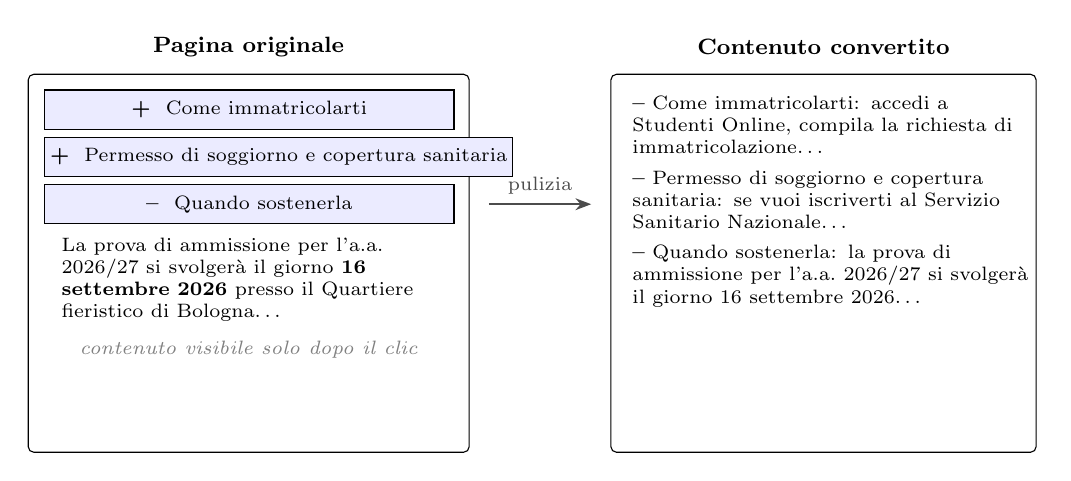
\begin{tikzpicture}[
      page/.style={draw, rounded corners=2pt, fill=white, inner sep=0pt},
      acc/.style={draw, fill=blue!8, minimum width=5.2cm, minimum height=0.5cm, font=\scriptsize, anchor=west,
                  inner sep=2pt},
      body/.style={font=\scriptsize, align=left, text width=5.0cm, anchor=north west},
      arr/.style={-{Stealth[length=2mm]}, thick, black!70},
    ]
    % pagina originale
    \node[font=\footnotesize\bfseries] at (2.8,0.55) {Pagina originale};
    \draw[rounded corners=2pt, fill=white] (0,-4.6) rectangle (5.6,0.2);
    \node[acc] at (0.2,-0.25) {\textbf{+}\ \ Come immatricolarti};
    \node[acc] at (0.2,-0.85) {\textbf{+}\ \ Permesso di soggiorno e copertura sanitaria};
    \node[acc] at (0.2,-1.45) {\textbf{--}\ \ Quando sostenerla};
    \node[body] at (0.3,-1.75) {La prova di ammissione per l'a.a.\ 2026/27 si svolgerà il giorno
      \textbf{16 settembre 2026} presso il Quartiere fieristico di Bologna\dots};
    \node[font=\scriptsize\itshape, text=gray] at (2.8,-3.3) {contenuto visibile solo dopo il clic};

    \draw[arr] (5.85,-1.45) -- node[above, font=\scriptsize] {pulizia} (7.15,-1.45);

    % sezioni risultanti
    \node[font=\footnotesize\bfseries] at (10.1,0.55) {Contenuto convertito};
    \draw[rounded corners=2pt, fill=white] (7.4,-4.6) rectangle (12.8,0.2);
    \node[body, text width=5.1cm] at (7.55,0.05) {\textbf{--} Come immatricolarti: accedi a Studenti Online,
      compila la richiesta di immatricolazione\dots\\[3pt]
      \textbf{--} Permesso di soggiorno e copertura sanitaria: se vuoi iscriverti al Servizio Sanitario
      Nazionale\dots\\[3pt]
      \textbf{--} Quando sostenerla: la prova di ammissione per l'a.a.\ 2026/27 si svolgerà il giorno
      16 settembre 2026\dots};
  \end{tikzpicture}
  \caption{Voci della pagina \emph{Iscriversi al Corso} di Infermieristica. Il contenuto delle voci
  chiuse è presente nella pagina ma marcato come nascosto: senza la pulizia sarebbe stato scartato, e con esso la
  data della prova di ammissione; dopo la pulizia il contenuto di ogni voce è conservato insieme al suo titolo.}
  \label{fig:voci}
\end{figure}

\paragraph{Struttura affidata alla presentazione.} In una pagina web la struttura logica del contenuto non sempre è
espressa con gli elementi che la descrivono, come i titoli di sezione: spesso è affidata a componenti grafici, come
il titolo di una voce espandibile, che il browser mostra come un'intestazione ma che nel codice non lo è. Per lo
strumento di conversione quella struttura non esiste, e ciò che ne segue degrada i frammenti in due modi: il
contenuto di una voce viene fuso in un unico blocco, separando ad esempio un elenco dalla frase che lo introduce, e
gli elementi annidati nelle parti sbagliate si propagano, come una nota esplicativa inserita nell'intestazione di
una colonna, che diventa parte dell'intestazione e viene ripetuta su ogni riga della tabella
(Figura~\ref{fig:struttura-presentazione}). Prima della conversione,
questi componenti vengono quindi ricondotti alla struttura che rappresentano: il titolo di una voce espandibile
diventa un titolo di sezione e le note annidate vengono spostate fuori dalla struttura che altererebbero.

\begin{figure}[H]
  \centering
  \footnotesize
  \newcommand{\frag}[1]{\fbox{\parbox{0.95\linewidth}{\raggedright\scriptsize #1}}}
  \newcommand{\nota}[2]{{\color{#1}\scriptsize #2}}
  \textbf{(a) Voce espandibile con un elenco}\\[4pt]
  \begin{minipage}[t]{0.48\textwidth}
    \textit{Senza correzione: la voce resta un elemento di elenco}\\[3pt]
    \frag{\textbf{Frammento 1}\\ \ldots\ Avere l'esenzione e pagare meno tasse. Puoi ottenere un'esenzione totale o
      una riduzione delle tasse\ldots\ Hai l'esenzione totale della quota variabile e paghi solo 157,04 € se ti
      trovi in una delle seguenti condizioni: \ldots}\\[3pt]
    \frag{\textbf{Frammento 2}\\ -- l'indicatore della situazione economica del nucleo familiare è pari o
      inferiore a 27.000 €;\\ -- l'indicatore \ldots\ è pari o inferiore a 40.000 € e diventi genitore\ldots}\\[3pt]
    \nota{red!70!black}{L'elenco è separato dalla frase che lo introduce: il frammento 2 non dice a cosa servono le
      soglie.}
  \end{minipage}\hfill
  \begin{minipage}[t]{0.48\textwidth}
    \textit{Con la correzione: la voce diventa una sezione}\\[3pt]
    \frag{\textbf{Frammento}\quad\textit{Tasse ed esenzioni $>$ \ldots\ $>$ Avere l'esenzione e pagare meno
      tasse}\\[2pt] Hai l'esenzione totale della quota variabile e paghi solo 157,04 € se ti trovi in una delle
      seguenti condizioni:\\ -- l'indicatore della situazione economica del nucleo familiare è pari o inferiore a
      27.000 €;\\ -- l'indicatore \ldots\ è pari o inferiore a 40.000 € e diventi genitore\ldots}\\[3pt]
    \nota{green!40!black}{Frase introduttiva ed elenco restano nello stesso frammento, sotto il titolo della
      voce.}
  \end{minipage}

  \vspace{12pt}
  \textbf{(b) Nota a comparsa nell'intestazione di una colonna}\\[4pt]
  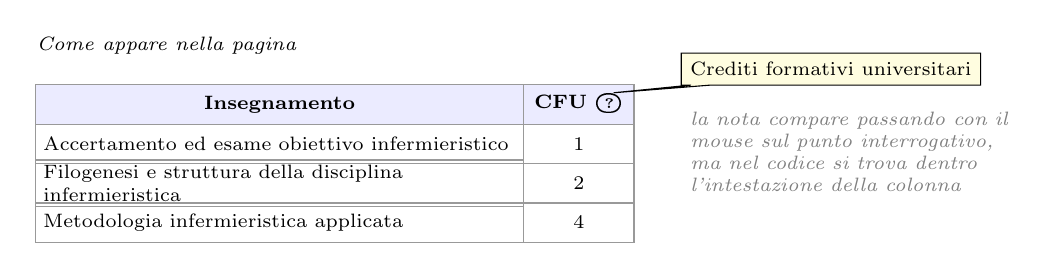
\begin{tikzpicture}[
      cell/.style={draw=black!40, minimum height=0.5cm, font=\scriptsize, inner sep=2pt},
      hd/.style={cell, fill=blue!8, font=\scriptsize\bfseries},
    ]
    \node[font=\scriptsize\itshape, anchor=west] at (-0.1,0.75) {Come appare nella pagina};
    \node[hd, minimum width=6.2cm, anchor=west] at (0,0) {Insegnamento};
    \node[hd, minimum width=1.4cm, anchor=west] (cfu) at (6.2,0) {CFU \textcircled{\tiny ?}};
    \foreach \y/\n/\c in {-0.5/Accertamento ed esame obiettivo infermieristico/1,
                          -1.0/Filogenesi e struttura della disciplina infermieristica/2,
                          -1.5/Metodologia infermieristica applicata/4} {
      \node[cell, minimum width=6.2cm, anchor=west, align=left, text width=6.0cm] at (0,\y) {\n};
      \node[cell, minimum width=1.4cm, anchor=west] at (6.2,\y) {\c};
    }
    \node[draw, rectangle callout, callout absolute pointer={(7.35,0.15)}, fill=yellow!12, font=\scriptsize,
          anchor=west] at (8.2,0.45) {Crediti formativi universitari};
    \node[font=\scriptsize\itshape, text=gray, anchor=west, text width=4.2cm] at (8.2,-0.6)
      {la nota compare passando con il mouse sul punto interrogativo, ma nel codice si trova dentro
      l'intestazione della colonna};
  \end{tikzpicture}\\[8pt]
  \begin{minipage}[t]{0.48\textwidth}
    \textit{Senza correzione: la nota è nell'intestazione}\\[3pt]
    \frag{Accertamento ed esame obiettivo infermieristico, \textbf{CFU ? Crediti formativi universitari} = 1\\
      Filogenesi e struttura della disciplina infermieristica, \textbf{CFU ? Crediti formativi universitari} = 2\\
      Metodologia infermieristica applicata, \textbf{CFU ? Crediti formativi universitari} = 4}\\[3pt]
    \nota{red!70!black}{La nota si ripete accanto a ogni insegnamento: in una tabella con decine di righe e note
      lunghe, il frammento si riempie di testo ripetuto.}
  \end{minipage}\hfill
  \begin{minipage}[t]{0.48\textwidth}
    \textit{Con la correzione: la nota diventa una legenda}\\[3pt]
    \frag{\texttt{| insegnamento | cfu |}\\
      \texttt{| Accertamento ed esame \ldots\ | 1 |}\\
      \texttt{| Filogenesi e struttura \ldots\ | 2 |}\\
      \texttt{| Metodologia infermieristica \ldots\ | 4 |}\\[2pt]
      Legenda -- cfu: Crediti formativi universitari}\\[3pt]
    \nota{green!40!black}{La nota compare una sola volta, subito dopo la tabella.}
  \end{minipage}
  \caption{Due effetti di una struttura affidata alla presentazione, ricostruiti in forma schematica su pagine del
  corpus del prototipo: (a) la voce \emph{Avere l'esenzione e pagare meno tasse} della pagina delle tasse di ateneo;
  (b) una tabella del piano didattico di Infermieristica (estratto: tre insegnamenti e la colonna dei crediti). A sinistra i frammenti senza la correzione, a destra
  quelli effettivamente indicizzati.}
  \label{fig:struttura-presentazione}
\end{figure}

Le regole con cui questi problemi vengono individuati dipendono da come è costruito un sito, e sono state definite
sui siti dell'ateneo; indicizzare pagine con una struttura diversa può richiederne di nuove, mentre il resto della
pipeline lavora sulla rappresentazione comune prodotta dalla conversione ed è indipendente dal sito di provenienza.

\subsection{Conversione in un formato strutturato}

Pagine web e documenti vengono convertiti con Docling~\cite{docling2024}, uno strumento open source che trasforma
documenti di formati diversi --- tra gli altri PDF, documenti Word, presentazioni PowerPoint, fogli di calcolo, pagine
HTML, Markdown e immagini --- in un'unica rappresentazione strutturata, il \emph{DoclingDocument}, salvata in formato
JSON. Il prototipo abilita PDF, DOCX, PPTX e HTML, i formati delle fonti indicizzate; gli altri formati supportati da
Docling si aggiungono estendendo l'elenco dei formati accettati dal convertitore, senza modifiche agli stadi
successivi, che lavorano sulla rappresentazione comune. A differenza di un'estrazione del solo testo, questa rappresentazione
conserva la struttura del documento: la gerarchia di titoli e sezioni, i paragrafi, gli elenchi, le tabelle con le
loro righe e colonne e le immagini, ciascuna con la propria posizione nel documento. Grazie a questa struttura,
nel passo successivo il documento può essere diviso in frammenti nei punti in cui finisce una sezione, un paragrafo
o una tabella, invece che ogni tot parole: si evita così di tagliare una frase o una tabella a metà.

La conversione si adatta al formato. Documenti Word e presentazioni contengono già una struttura esplicita ---
stili dei titoli, paragrafi, tabelle, diapositive --- che Docling legge direttamente dal file. I PDF, invece, non
contengono una struttura esplicita ma solo testo e grafica posizionati sulla pagina: Docling ne ricostruisce la
struttura con modelli di analisi del layout, che riconoscono titoli, paragrafi, tabelle e immagini; il
riconoscimento ottico dei caratteri (OCR) recupera il testo contenuto nelle immagini delle pagine, e un modello
dedicato ricostruisce righe e colonne delle tabelle. La correttezza delle tabelle è particolarmente importante nel
dominio di questo lavoro, perché è in forma di tabella che l'ateneo pubblica scadenze, importi e calendari: una
cella attribuita alla colonna sbagliata produce una data o un importo errato nella risposta.

La Figura~\ref{fig:docling-pdf} mostra il primo passaggio su un documento reale. L'analisi del layout assegna a
ogni elemento della pagina un ruolo --- titolo, paragrafo, tabella, didascalia, piè di pagina --- e ne ricava
l'ordine di lettura e la gerarchia delle sezioni; gli elementi ripetuti su ogni pagina, come il piè di pagina,
vengono riconosciuti e tenuti fuori dal testo. Il riconoscimento ottico dei caratteri (OCR) recupera invece il testo
che non esiste come tale nel file perché fa parte di un'immagine, ad esempio le etichette di un diagramma o una
pagina scansionata. Il risultato è affidabile per le singole parole, ma non per la loro disposizione: in un
diagramma il testo non segue righe ordinate, e frasi appartenenti a riquadri diversi finiscono nello stesso blocco.
Per questo, nei diagrammi, il testo dell'OCR è affiancato da una descrizione dell'immagine nel suo insieme,
discussa nel paragrafo seguente.

\begin{figure}[H]
  \centering
  \textbf{\footnotesize (a) Analisi del layout di una pagina PDF}\\[6pt]
  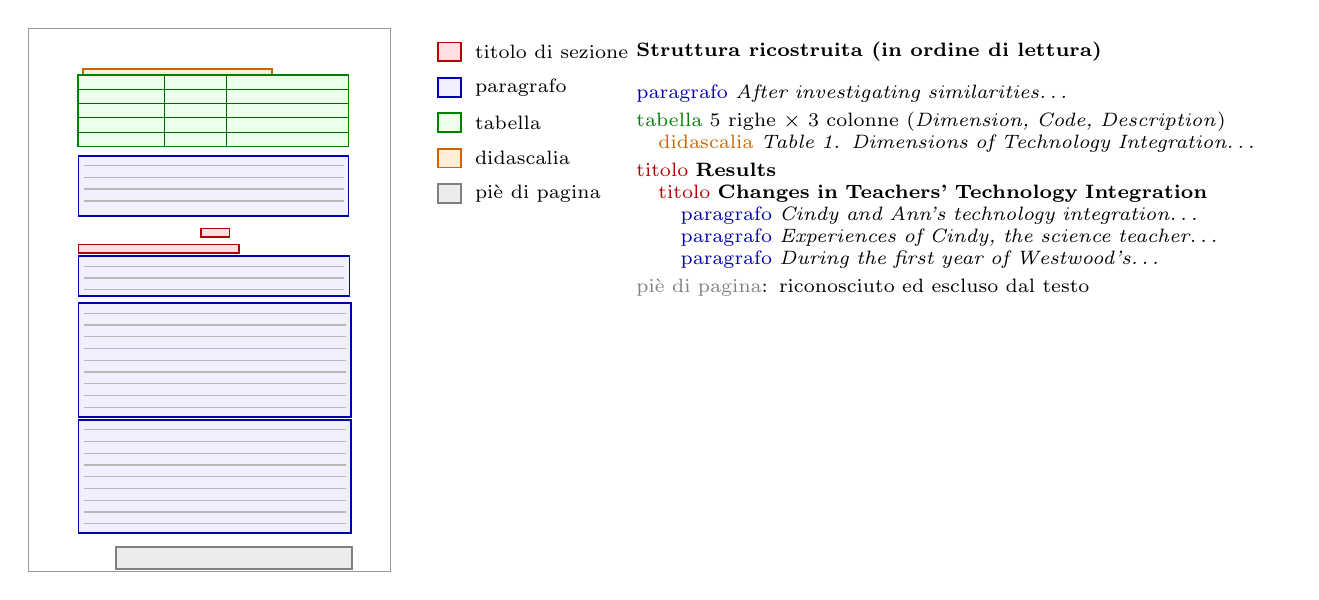
\begin{tikzpicture}[
      hd/.style={draw=red!70!black, fill=red!12, line width=0.6pt},
      tx/.style={draw=blue!70!black, fill=blue!6, line width=0.6pt},
      capt/.style={draw=orange!80!black, fill=orange!15, line width=0.6pt},
      tab/.style={draw=green!50!black, fill=green!8, line width=0.6pt},
      ft/.style={draw=gray, fill=gray!15, line width=0.6pt},
      txl/.style={gray!55, line width=0.5pt},
      tabl/.style={green!40!black, line width=0.3pt},
      leg/.style={font=\scriptsize, anchor=west},
      tree/.style={font=\scriptsize, anchor=west, align=left},
    ]
    \draw[black!40, fill=white] (0,0) rectangle (4.600,6.900);
    \draw[hd] (2.194,4.249) rectangle (2.556,4.355);
    \draw[hd] (0.639,4.046) rectangle (2.673,4.153);
    \draw[tx] (0.639,4.515) rectangle (4.068,5.281);
    \draw[txl] (0.703,5.154) -- (4.004,5.154);
    \draw[txl] (0.703,5.005) -- (4.004,5.005);
    \draw[txl] (0.703,4.856) -- (4.004,4.856);
    \draw[txl] (0.703,4.706) -- (4.004,4.706);
    \draw[tx] (0.639,3.503) rectangle (4.078,4.004);
    \draw[txl] (0.703,3.876) -- (4.014,3.876);
    \draw[txl] (0.703,3.727) -- (4.014,3.727);
    \draw[txl] (0.703,3.578) -- (4.014,3.578);
    \draw[tx] (0.639,1.959) rectangle (4.100,3.407);
    \draw[txl] (0.703,3.280) -- (4.036,3.280);
    \draw[txl] (0.703,3.131) -- (4.036,3.131);
    \draw[txl] (0.703,2.981) -- (4.036,2.981);
    \draw[txl] (0.703,2.832) -- (4.036,2.832);
    \draw[txl] (0.703,2.683) -- (4.036,2.683);
    \draw[txl] (0.703,2.534) -- (4.036,2.534);
    \draw[txl] (0.703,2.385) -- (4.036,2.385);
    \draw[txl] (0.703,2.236) -- (4.036,2.236);
    \draw[txl] (0.703,2.087) -- (4.036,2.087);
    \draw[tx] (0.639,0.490) rectangle (4.100,1.927);
    \draw[txl] (0.703,1.800) -- (4.036,1.800);
    \draw[txl] (0.703,1.650) -- (4.036,1.650);
    \draw[txl] (0.703,1.501) -- (4.036,1.501);
    \draw[txl] (0.703,1.352) -- (4.036,1.352);
    \draw[txl] (0.703,1.203) -- (4.036,1.203);
    \draw[txl] (0.703,1.054) -- (4.036,1.054);
    \draw[txl] (0.703,0.905) -- (4.036,0.905);
    \draw[txl] (0.703,0.756) -- (4.036,0.756);
    \draw[txl] (0.703,0.607) -- (4.036,0.607);
    \draw[capt] (0.692,6.314) rectangle (3.099,6.378);
    \draw[tab] (0.628,5.399) rectangle (4.068,6.304);
    \draw[ft] (1.118,0.032) rectangle (4.110,0.309);
    \draw[tabl] (0.628,6.123) -- (4.068,6.123);
    \draw[tabl] (0.628,5.942) -- (4.068,5.942);
    \draw[tabl] (0.628,5.761) -- (4.068,5.761);
    \draw[tabl] (0.628,5.580) -- (4.068,5.580);
    \draw[tabl] (1.729,5.399) -- (1.729,6.304);
    \draw[tabl] (2.520,5.399) -- (2.520,6.304);
    % legenda
    \foreach \y/\st/\t in {6.6/hd/titolo di sezione, 6.15/tx/paragrafo, 5.7/tab/tabella, 5.25/capt/didascalia,
                           4.8/ft/piè di pagina} {
      \draw[\st] (5.2,\y-0.12) rectangle (5.5,\y+0.12);
      \node[leg] at (5.55,\y) {\t};
    }
    % struttura risultante
    \node[font=\scriptsize\bfseries, anchor=west] at (7.6,6.6) {Struttura ricostruita (in ordine di lettura)};
    \node[tree, anchor=north west, text width=8.2cm] at (7.6,6.3) {%
      \textcolor{blue!70!black}{paragrafo} \emph{After investigating similarities\dots}\\[2pt]
      \textcolor{green!50!black}{tabella} 5 righe $\times$ 3 colonne (\emph{Dimension, Code, Description})\\
      \quad\textcolor{orange!80!black}{didascalia} \emph{Table 1. Dimensions of Technology Integration\dots}\\[2pt]
      \textcolor{red!70!black}{titolo} \textbf{Results}\\
      \quad\textcolor{red!70!black}{titolo} \textbf{Changes in Teachers' Technology Integration}\\
      \qquad\textcolor{blue!70!black}{paragrafo} \emph{Cindy and Ann's technology integration\dots}\\
      \qquad\textcolor{blue!70!black}{paragrafo} \emph{Experiences of Cindy, the science teacher\dots}\\
      \qquad\textcolor{blue!70!black}{paragrafo} \emph{During the first year of Westwood's\dots}\\[2pt]
      \textcolor{gray}{piè di pagina}: riconosciuto ed escluso dal testo};
  \end{tikzpicture}
  \caption{Conversione di un PDF con Docling, ridisegnata dai dati prodotti dalla conversione di un documento del
  corpus del prototipo. L'analisi del layout riconosce gli elementi della pagina, qui la pagina 9 di un
  articolo scientifico, e ne ricostruisce la gerarchia e l'ordine di lettura; il piè di pagina viene escluso dal
  testo.}
  \label{fig:docling-pdf}
\end{figure}

\paragraph{Descrizione delle immagini.} Documenti come slide e dispense contengono spesso diagrammi e schemi il
cui contenuto non è espresso nel testo circostante. Per renderlo ricercabile, ogni immagine estratta durante la
conversione viene descritta a parole da un modello linguistico capace di interpretare immagini, e la descrizione
viene inserita nel documento al posto dell'immagine stessa (Figura~\ref{fig:descrizione-immagine}). 

Il sistema usa quindi due modelli linguistici distinti: un modello multimodale, Qwen2.5-VL-7B-Instruct, che descrive
le immagini durante la conversione, e un modello solo testuale che genera le risposte. Un unico
modello multimodale per entrambi i compiti sarebbe stato più semplice da gestire, ma è stato scartato per quattro
ragioni.

\begin{itemize}
  \item \textbf{Taglia a parità di memoria.} A parità di risorse, un modello multimodale dedica una parte della
  propria capacità all'elaborazione delle immagini, e le versioni multimodali disponibili per famiglia sono meno
  numerose: per Qwen2.5 esistono in taglie da 3, 7, 32 e 72 miliardi di parametri. Con una GPU da 16~GB la più grande
  utilizzabile è quella da 7 miliardi, mentre il modello solo testuale arriva a 14 miliardi. Come discusso nella
  Sezione~\ref{sec:llm} (Figura~\ref{fig:scaling}), a parità di famiglia la taglia è il fattore che più incide sulla qualità delle risposte.
  \item \textbf{Le immagini servono una volta sola.} Il contenuto di un'immagine viene trasformato in testo durante
  la conversione e da quel momento è parte del frammento come qualunque altro paragrafo: ricercabile dal recupero e
  leggibile dal modello delle risposte. Saper interpretare le immagini è quindi necessario una volta per documento,
  al momento dell'indicizzazione, e non a ogni domanda.
  \item \textbf{Spazio nel contesto.} Passare le immagini al modello anche al momento della risposta avrebbe un costo
  diretto: ogni immagine occupa nel contesto centinaia di token, che con una finestra di 8.192 token andrebbero
  sottratti ai frammenti di testo, a vantaggio di una piccola minoranza di domande riferite a un'immagine.
  \item \textbf{Requisiti diversi.} La descrizione delle immagini è un'elaborazione fuori linea, in cui il tempo
  conta poco, mentre la generazione delle risposte deve essere rapida e sempre disponibile. Tenere separati i due
  modelli permette di avviare il modello multimodale, con una seconda istanza di vLLM, solo per la durata della
  conversione, senza fermare l'assistente mentre nuovi documenti vengono elaborati.
\end{itemize}

 Il modello
riceve un'istruzione che chiede di riportare gli elementi principali di un diagramma e le loro relazioni, il testo
leggibile e i valori di eventuali grafici. Le immagini più piccole di una soglia di area vengono ignorate, perché si tratta in
genere di loghi ed elementi decorativi; la soglia predefinita dello strumento, pensata per pagine di testo, è stata
però abbassata di dieci volte, perché su una slide un diagramma significativo occupa spesso meno del 2\% della
pagina e sarebbe stato scartato. In Docling la descrizione delle immagini fa parte dell'elaborazione dei PDF: le
immagini di documenti Word e presentazioni vengono estratte ma non descritte, e le presentazioni con contenuto
visivo rilevante conviene quindi indicizzarle esportate in PDF.

\begin{figure}[H]
  \centering
  \begin{minipage}[c]{0.42\textwidth}
    \centering
    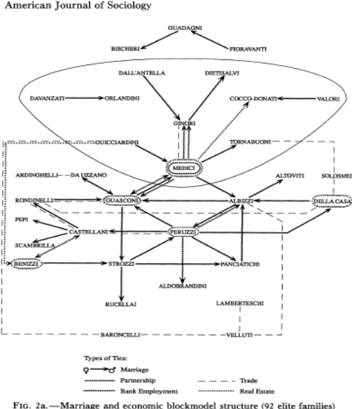
\includegraphics[width=\textwidth]{assets/famiglie_fiorentine.png}
  \end{minipage}\hfill
  \begin{minipage}[c]{0.54\textwidth}
    \footnotesize\itshape
    ``L'immagine mostra una struttura blocchi economiche-matrimoniali basata su 92 famiglie elite, come illustra la
    figura `Fig.~2a' dell'American Journal of Sociology. Il diagramma rappresenta una rete complessa che collega
    diversi nomi di famiglie aristocratiche italiane, indicando le relazioni matrimoniali e economiche tra esse.
    [\dots] Al centro si trova l'elemento `MEDICI', da cui partono numerose frecce verso altre famiglie,
    simbolizzando il dominio economico e matrimoniale della famiglia Medici sulla restante élite\dots''
  \end{minipage}
  \caption{Una figura tratta dalle slide di un insegnamento, la rete dei legami matrimoniali ed economici tra le
  famiglie dell'élite fiorentina (a sinistra), e un estratto della descrizione generata durante la conversione (a
  destra), che entra nel frammento indicizzato al posto dell'immagine. Grazie alla descrizione, una domanda come
  ``quale famiglia occupa la posizione centrale della rete?'' trova la risposta anche se il nome non compare nel
  testo della slide.}
  \label{fig:descrizione-immagine}
\end{figure}

La descrizione automatica rende ricercabile un contenuto che altrimenti non lo sarebbe, ma non è sempre fedele, e
il suo errore più insidioso non è l'omissione ma l'invenzione. La stessa descrizione della
Figura~\ref{fig:descrizione-immagine}, dopo aver colto correttamente l'insieme del diagramma, prosegue elencando
alcuni legami tra famiglie: afferma che la famiglia Valori è ``collegata direttamente'' ai Medici, mentre nel
diagramma è collegata ai Cocco-Donati; attribuisce alla famiglia Dall'Antella ``due figli sposati con membri delle
famiglie Orlandini e Coccolonati'', una famiglia che nel diagramma non compare; trasforma Altoviti in
``Aldoviti''. Sono affermazioni precise, formulate con la stessa sicurezza di quelle corrette e indistinguibili da
esse per chi legge il testo indicizzato: una domanda sui legami della famiglia Valori recupererebbe questa
descrizione, e il modello delle risposte, che si attiene fedelmente al contesto ricevuto, riporterebbe l'errore
citandone anche la fonte. Per questo il testo generato a partire dalle immagini va considerato meno affidabile di quello estratto
direttamente dai documenti, e la sua accuratezza è valutata separatamente, con domande dedicate alle immagini, nel
Capitolo~\ref{cap:validazione}.

\paragraph{La taglia del modello multimodale.} La qualità delle descrizioni dipende in misura decisiva dalla taglia
del modello che le produce. Per verificarlo, la stessa immagine della Figura~\ref{fig:descrizione-immagine} è stata
descritta anche da SmolVLM-256M, un modello multimodale da 256 milioni di parametri, circa trenta volte più piccolo
di quello adottato e abbastanza leggero da poter essere eseguito senza GPU dedicata: è il tipo di modello che si
sceglierebbe per non sottrarre risorse al resto del sistema, ed è quello provato inizialmente nel prototipo. La
Tabella~\ref{tab:taglia-vlm} riporta le descrizioni ottenute.

\begin{table}[H]
  \centering
  \footnotesize
  \begin{tabularx}{\textwidth}{@{} L{3.3cm} >{\raggedright\arraybackslash\itshape}X @{}}
    \toprule
    \textbf{Modello} & \textbf{\upshape Descrizione prodotta} \\
    \midrule
    SmolVLM-256M &
      In the image, we can see there is an object with some text and images attached to it. We can also see some
      arrows on the objects. There are trees at the top of the image. \\[3pt]
    Qwen2.5-VL-7B &
      L'immagine mostra una struttura blocchi economiche-matrimoniali basata su 92 famiglie elite [\dots] Il
      diagramma rappresenta una rete complessa che collega diversi nomi di famiglie aristocratiche italiane,
      indicando le relazioni matrimoniali e economiche tra esse. [\dots] Al centro si trova l'elemento `MEDICI',
      da cui partono numerose frecce verso altre famiglie\dots \\
    \bottomrule
  \end{tabularx}
  \caption{Descrizioni della rete delle famiglie fiorentine (Figura~\ref{fig:descrizione-immagine}) prodotte da
  due modelli multimodali di taglia diversa.}
  \label{tab:taglia-vlm}
\end{table}

Il modello piccolo fallisce producendo una descrizione generica e in parte inventata. Il modello da
7 miliardi di parametri coglie invece la natura del diagramma, la sua fonte e l'informazione principale, la
posizione centrale della famiglia Medici, che è proprio ciò che una domanda su questa immagine chiederebbe. Gli
errori di dettaglio visti sopra mostrano che la taglia maggiore riduce il problema senza eliminarlo, ma la
differenza tra le due taglie non è trascurabile: è la differenza tra una descrizione utile, da verificare, e una
inutilizzabile. È questa la ragione per cui il prototipo dedica alle descrizioni un modello multimodale di taglia
media, su una GPU propria, anziché un modello minimo; la penalità sulle ripetizioni è mantenuta anche con il modello
più grande, come ulteriore protezione contro i cicli di ripetizione.

\paragraph{Normalizzazione.} La ricostruzione della struttura di un PDF è un'operazione statistica e non è
perfetta. Alcuni dei suoi errori sono occasionali, ma altri si ripetono in modo sistematico e, poiché la
suddivisione in frammenti si basa proprio su quella struttura, si propagano a tutti i passi successivi. Dopo la
conversione, ogni documento viene quindi corretto da regole che affrontano quattro tipi di errore ricorrenti:
\begin{itemize}
  \item \textbf{titoli riconosciuti in modo errato}: un titolo classificato come testo ordinario, o diviso su due
  intestazioni, o fuso con il titolo successivo, altera la gerarchia delle sezioni, e con essa i punti in cui il
  documento viene diviso in frammenti e il percorso delle intestazioni che li accompagna. È il caso tipico dei documenti normativi, come i
  regolamenti, in cui un titolo d'articolo (``Art.~5'') viene spesso letto come un paragrafo;
  \item \textbf{elementi ripetuti di pagina}: intestazioni e piè di pagina che lo strumento non ha riconosciuto come
  tali compaiono come testo nel corpo del documento, una volta per pagina; vengono individuati perché ripetuti
  identici più volte nello stesso documento, e rimossi;
  \item \textbf{paragrafi spezzati}: un cambio di pagina o di colonna spezza un paragrafo a metà frase in due
  blocchi, che finirebbero in frammenti diversi; i blocchi consecutivi che non terminano con una punteggiatura di
  fine frase vengono ricomposti;
  \item \textbf{tabelle divise}: una tabella che prosegue sulla pagina successiva viene restituita come due tabelle
  distinte, la seconda senza intestazioni di colonna; le due parti vengono riunite, perché una tabella di scadenze o
  di importi deve restare intera per essere interpretata correttamente.
\end{itemize}

\subsection{Suddivisione in frammenti}\label{sec:chunking}

Il documento convertito viene suddiviso in frammenti con una strategia di \emph{chunking strutturale} ibrida
(Sezione~\ref{sec:rag}), offerta da Docling stesso: il documento viene diviso nei punti in cui finisce una
sezione, un paragrafo, un elenco o una tabella, e solo le parti che superano la dimensione massima vengono
ulteriormente suddivise, mentre parti consecutive troppo brevi sotto la stessa intestazione vengono riunite. La dimensione massima
di un frammento è di 512 token, contati con lo stesso tokenizzatore del modello di embedding, così che il conteggio
coincida con quello che il modello vedrà effettivamente. Il valore è stato scelto sperimentalmente: con frammenti
di 256 token la risposta si spezza più spesso tra frammenti diversi e il recupero peggiora sensibilmente, mentre
con 768 token i risultati restano equivalenti.

Ogni frammento conserva il \emph{percorso delle intestazioni} della sezione da cui proviene, ad esempio
\emph{Prova finale: modalità e scadenze $>$ SCADENZE}. Il percorso è essenziale per frammenti che, letti da soli,
sarebbero ambigui: una riga come ``Estivo: 2 giugno 2026, 19 giugno 2026\dots'' acquista significato solo sapendo
che appartiene al calendario delle scadenze della prova finale. Per questo il percorso viene incluso sia nella
rappresentazione vettoriale del frammento sia nel testo valutato dal modello di reranking. Non viene invece
introdotta alcuna sovrapposizione tra frammenti consecutivi. Quando si taglia ogni tot parole è utile ripetere
l'ultima parte di un frammento all'inizio del successivo, perché il taglio può cadere a metà di una frase; qui
invece il taglio cade sempre alla fine di una sezione, di un paragrafo o di una tabella, e il contesto più ampio di
un frammento è comunque recuperabile attraverso la sua sezione di appartenenza, come descritto più avanti.

Tre ulteriori interventi affrontano problemi ricorrenti nei contenuti amministrativi e didattici.

\begin{itemize}
  \item \textbf{Tabelle.} Scadenze, importi e calendari sono pubblicati quasi sempre in forma di tabella, ma il
  modo in cui una tabella è scritta raramente corrisponde al modo in cui viene interrogata. Le intestazioni sono
  spesso in maiuscolo e le date in forma numerica, mentre chi pone una domanda scrive ``l'appello di ottobre'' o ``il
  16 luglio'': la distanza lessicale abbassa la pertinenza che il recupero attribuisce alla tabella, proprio per le
  domande a cui risponde. Le tabelle vengono quindi riscritte nella forma delle domande usando
  date per esteso (Figura~\ref{fig:tabella-leggibile}). L'effetto è misurabile: per la domanda ``scadenza della domanda
  di laurea tardiva per l'appello di ottobre'', la pertinenza attribuita dal reranker alla tabella delle scadenze
  passa da 0,589 a 0,840.
  \item \textbf{Frammenti troppo brevi.} Un frammento di poche parole, tipicamente la frase introduttiva di una
  sezione senza altri frammenti con cui essere riunito, è poco distintivo per il recupero; i frammenti sotto i 40
  token vengono quindi accorpati al frammento adiacente.
  \item \textbf{Collegamenti.} I collegamenti ipertestuali vengono ridotti al solo testo visibile, eliminando
  l'indirizzo: un frammento riporta ``simula l'importo delle tasse'' anziché un lungo URL che non aggiunge
  significato e consuma spazio.
\end{itemize}

\begin{figure}[H]
  \centering
  \begin{minipage}{\textwidth}
    \textbf{\footnotesize Prima}\\[2pt]
    \fbox{\parbox{0.97\textwidth}{\ttfamily\scriptsize
      | **SCADENZA PRESENTAZIONE DOMANDA DI LAUREA** | **SCADENZA DOMANDA DI LAUREA TARDIVA** | **APPELLO DI LAUREA** |\\
      | - | - | - |\\
      | 04/06/2026 | 18/06/2026 | 16/07/2026 |\\
      | 19/08/2026 | 03/09/2026 | 01/10/2026 |}}\\[6pt]
    \textbf{\footnotesize Dopo}\\[2pt]
    \fbox{\parbox{0.97\textwidth}{\ttfamily\scriptsize
      | scadenza presentazione domanda di laurea | scadenza domanda di laurea tardiva | appello di laurea |\\
      | - | - | - |\\
      | 4 giugno 2026 | 18 giugno 2026 | 16 luglio 2026 |\\
      | 19 agosto 2026 | 3 settembre 2026 | 1 ottobre 2026 |}}
  \end{minipage}
  \caption{Riscrittura di una tabella delle scadenze della prova finale di Ingegneria e scienze informatiche: date per esteso, nella forma in cui compaiono
  nelle domande degli studenti. Il testo ``Dopo'' è quello effettivamente indicizzato.}
  \label{fig:tabella-leggibile}
\end{figure}

\paragraph{Sezioni e fusione gerarchica.} Oltre ai frammenti, che sono le unità effettivamente indicizzate e
confrontate con la domanda, il sistema conserva anche le \emph{sezioni} a cui appartengono: per ogni sezione divisa
in almeno due frammenti viene costruito un nodo che li raggruppa (Figura~\ref{fig:frammenti-sezioni}). Le sezioni
non vengono indicizzate, ma servono al recupero per la fusione gerarchica (Sezione~\ref{sec:rag}): quando tra i
frammenti selezionati per una domanda ne compaiono abbastanza della stessa sezione, questi vengono sostituiti dalla
sezione intera, così che il modello riceva un contesto completo e coerente invece di parti isolate.

\begin{figure}[H]
  \centering
  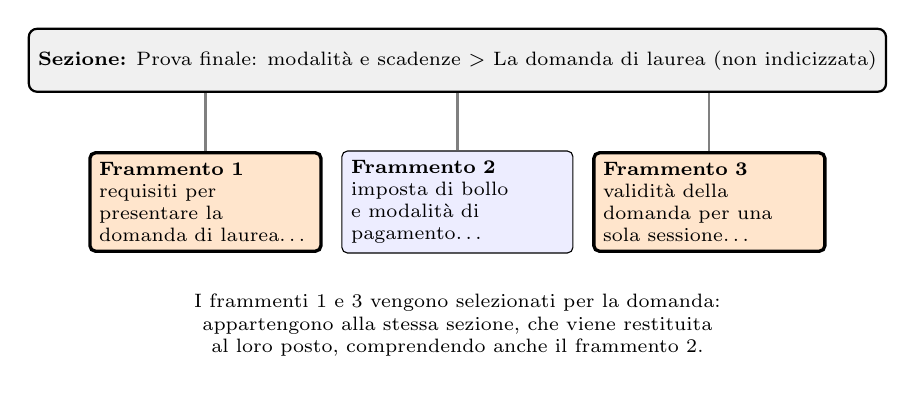
\begin{tikzpicture}[
      sec/.style={draw, thick, rounded corners=3pt, fill=gray!12, align=center, font=\scriptsize,
                  minimum width=9.2cm, minimum height=0.8cm},
      leaf/.style={draw, rounded corners=2pt, fill=blue!7, align=left, font=\scriptsize, text width=2.7cm,
                   minimum height=1.25cm},
      sel/.style={leaf, fill=orange!20, very thick},
      arr/.style={-{Stealth[length=2mm]}, thick, black!70},
    ]
    \node[sec] (s) at (0,0) {\textbf{Sezione:} Prova finale: modalità e scadenze $>$ La domanda di laurea (non
      indicizzata)};
    \node[sel] (f1) at (-3.2,-1.8) {\textbf{Frammento 1}\\ requisiti per presentare la domanda di laurea\dots};
    \node[leaf] (f2) at (0,-1.8) {\textbf{Frammento 2}\\ imposta di bollo e modalità di pagamento\dots};
    \node[sel] (f3) at (3.2,-1.8) {\textbf{Frammento 3}\\ validità della domanda per una sola sessione\dots};
    \foreach \f in {f1,f2,f3} \draw[thick, black!50] (s.south -| \f.north) -- (\f.north);
    \node[font=\scriptsize, align=center, text width=9.5cm, anchor=north] at (0,-2.85)
      {I frammenti 1 e 3 vengono selezionati per la domanda: appartengono alla stessa sezione, che viene
      restituita al loro posto, comprendendo anche il frammento 2.};
  \end{tikzpicture}
  \caption{Frammenti e sezioni. Solo i frammenti vengono indicizzati e confrontati con la domanda; le sezioni
  permettono di restituire al modello un contesto più ampio quando più frammenti della stessa sezione risultano
  pertinenti.}
  \label{fig:frammenti-sezioni}
\end{figure}

La lunghezza dei frammenti dipende dal tipo di fonte. Le sezioni delle pagine web sono in genere più brevi del
limite e restano in un unico frammento, mentre le sezioni lunghe di regolamenti, dispense e pagine più estese vengono
suddivise: nel corpus del prototipo, ad esempio, i frammenti hanno una lunghezza mediana di 117 token, ben al di
sotto del limite di 512.

\subsection{Metadati}\label{sec:metadati}

A ogni frammento viene associato un insieme di metadati, riportati nella Tabella~\ref{tab:metadati} per un
frammento del materiale del corso di Tecniche di Consulenza nella Scuola, relativo al \emph{Change Laboratory}. I
metadati di corso vengono ricavati dalla posizione del documento nell'albero delle cartelle prodotto
dall'acquisizione: per i documenti di un corso, pagine web o file, i livelli del percorso indicano il tipo di
laurea, il corso, la sezione e, per i materiali didattici, l'insegnamento; i documenti di ateneo, che seguono
un'organizzazione diversa, ricevono invece l'indicazione \emph{ateneo} e nessun corso. È su questi due campi, ambito
e corso, che si basa la gestione dei corsi: limitare la ricerca alle
pagine di ateneo e a quelle del corso dello studente, e privilegiare queste ultime.

\begin{table}[H]
  \centering
  \small
  \begin{tabularx}{\textwidth}{@{} l >{\raggedright\arraybackslash}X >{\raggedright\arraybackslash}X @{}}
    \toprule
    \textbf{Campo} & \textbf{Significato} & \textbf{Esempio} \\
    \midrule
    ambito & documento di un corso o di ateneo & corso \\
    tipo di laurea & laurea, laurea magistrale & laurea magistrale \\
    corso & corso di laurea a cui appartiene il documento & PsicologiaScolasticaComunita \\
    sezione & sezione del sito o cartella da cui proviene il documento & corsi \\
    insegnamento & insegnamento a cui si riferisce un materiale didattico & TecnicheDiConsulenzaNellaScuola \\
    intestazioni & percorso dei titoli della sezione & Change Laboratory (Change Lab) \\
    URL di provenienza & indirizzo della pagina web originale, mostrato tra le fonti &
      --- (materiale didattico caricato come file, non pagina web) \\
    identificativo & ricavato in modo stabile dal percorso del documento & 3e53833e-ffc7-5e84-ab82-9a13a6776148 \\
    impronta del contenuto & firma del file originale, per riconoscerne le modifiche & 8e837f4622a5b4e2 \\
    immagini & immagini associate al frammento, se presenti & --- (nessuna in questo frammento) \\
    \bottomrule
  \end{tabularx}
  \caption{Metadati associati a ogni frammento, con i valori reali di un frammento del materiale didattico del corso
  di Tecniche di Consulenza nella Scuola, sul metodo del \emph{Change Laboratory}: a differenza di una pagina web
  crawlata, un materiale didattico caricato come file non ha un URL di provenienza, ma valorizza il campo
  insegnamento.}
  \label{tab:metadati}
\end{table}

\paragraph{Aggiornamento incrementale.} Pagine e documenti dell'ateneo cambiano nel tempo, ad esempio a ogni nuovo anno
accademico, e ripetere l'intera preparazione a ogni modifica sarebbe inutilmente costoso, soprattutto per i PDF, la cui
conversione richiede l'analisi del layout, l'OCR e la descrizione delle immagini. Ogni frammento conserva quindi
l'impronta del documento da cui proviene, calcolata sul file originale. A ogni nuova esecuzione vengono elaborati
solo i documenti nuovi e quelli la cui impronta è cambiata; per questi ultimi, i frammenti precedenti vengono prima
eliminati sia dall'archivio sia dal database vettoriale, così che la versione aggiornata li sostituisca invece di
affiancarsi a quella superata. L'identificativo di ogni documento è ricavato in modo deterministico dal suo
percorso, così che lo stesso documento mantenga lo stesso identificativo da un'esecuzione all'altra.


\section{Embedding}\label{sec:embedding}

Tra l'indicizzazione e il recupero si colloca un componente condiviso dai due processi (Figura~\ref{fig:componenti}):
l'Embedding trasforma ogni frammento, al momento dell'indicizzazione, nella sua rappresentazione vettoriale, e la
stessa trasformazione viene applicata alla domanda di uno studente al momento del recupero, così che domanda e
frammenti siano confrontabili nello stesso spazio (Sezione~\ref{sec:rag}). Questa sezione descrive il modello usato,
cosa viene effettivamente trasformato in vettore e come viene conservato nel database vettoriale.

\subsection{Il modello: BGE-M3}

Il modello di embedding adottato è BGE-M3~\cite{chen2024bgem3}, già discusso nella Sezione~\ref{subsec:embedding}. La
scelta è motivata da una caratteristica specifica di questo modello più che dalla sola qualità delle sue
rappresentazioni: a differenza di un modello di embedding classico, che produce solo una rappresentazione densa, BGE-M3
ne produce tre nello stesso passaggio di calcolo --- una densa, una sparsa e una per token --- evitando così di dover addestrare, eseguire e
mantenere allineati modelli distinti per ciascun tipo di rappresentazione. Un secondo motivo è la finestra di
contesto del modello, fino a 8.192 token: più ampia del limite di 512 token scelto per un frammento, lascia margine a non troncare mai un frammento durante l'embedding, anche per quelli
risultanti da una fusione gerarchica di più frammenti originari.

A titolo di esempio, per il frammento della Tabella~\ref{tab:metadati} --- il materiale didattico del corso di
Tecniche di Consulenza nella Scuola sul \emph{Change Laboratory} --- BGE-M3 calcola, nello stesso passaggio, le tre
rappresentazioni seguenti:
\begin{itemize}
  \item una rappresentazione \textbf{densa} di 1.024 numeri in virgola mobile, le cui prime componenti sono, in
    questo caso, $-0{,}009,\ -0{,}036,\ 0{,}007,\ 0{,}022,\ -0{,}007,\ -0{,}028,\ \dots$;
  \item una rappresentazione \textbf{sparsa}, che assegna un peso ai soli token lessicalmente rilevanti del testo;
    la Tabella~\ref{tab:sparse-esempio} mette a confronto, per questo frammento, il peso di alcune parole chiave
    con quello, nullo, di un articolo e di una preposizione --- la rappresentazione sparsa distingue così le parole
    che portano significato da quelle puramente grammaticali;
  \item una rappresentazione \textbf{per token}, una matrice di 87 vettori da 1.024 numeri ciascuno --- uno per
    ogni token in cui il testo del frammento viene suddiviso --- usata dalla sola modalità di recupero con late
    interaction (Sezione~\ref{sec:rag}).
\end{itemize}

\begin{table}[H]
  \centering
  \small
  \begin{tabular}{@{} l r @{}}
    \toprule
    \textbf{Parola} & \textbf{Peso} \\
    \midrule
    \texttt{intervento} & 0,236 \\
    \texttt{consulenza} & 0,234 \\
    \texttt{Ciclo} & 0,148 \\
    \texttt{sviluppato} & 0,125 \\
    \midrule
    \texttt{il} & 0,000 \\
    \texttt{a} & 0,000 \\
    \bottomrule
  \end{tabular}
  \caption{Peso, nella rappresentazione sparsa del frammento \emph{Change Laboratory} della Tabella~\ref{tab:metadati},
  di quattro parole che portano significato contro quello di un articolo e di una preposizione: la rappresentazione
  sparsa assegna peso nullo alle seconde, pur comparendo entrambe nel testo.}
  \label{tab:sparse-esempio}
\end{table}

\subsection{Cosa viene trasformato in vettore}

Non tutto il testo associato a un frammento entra nella sua rappresentazione vettoriale. Il percorso delle
intestazioni della sezione di provenienza (Sezione~\ref{sec:chunking}) viene incluso, perché è spesso necessario a
rendere comprensibile un frammento altrimenti ambiguo; gli altri metadati --- corso, ambito, sezione, stato,
l'indirizzo della pagina di provenienza e gli altri campi della Tabella~\ref{tab:metadati} --- ne restano invece
esclusi, e intervengono solo più avanti, come filtri sul database vettoriale (Sezione~\ref{sec:ricerca-ibrida}), non
come parte del significato che l'embedding rappresenta: il nome del corso di un frammento, ad esempio, non deve
influenzare quanto quel frammento è semanticamente vicino a una domanda, un compito che spetta al filtro, non alla
rappresentazione vettoriale.

\subsection{Il database vettoriale: Qdrant}

Le rappresentazioni calcolate vengono salvate in Qdrant, il database vettoriale scelto per due capacità native che
evitano di doverle replicare lato applicazione. La prima è la fusione tra ricerca densa e sparsa con Reciprocal Rank
Fusion (Sezione~\ref{sec:rag}), eseguita da Qdrant stesso a partire da due vettori nominati distinti, \emph{dense} e
\emph{sparse}, associati allo stesso punto; un terzo vettore nominato, \emph{colbert}, multivettore con
confronto per massima similarità, ospita la rappresentazione per token usata dalla sola modalità di recupero con
late interaction. La seconda è l'indicizzazione dei campi del
payload --- stato, corso, ambito, tipo di laurea, sezione, insegnamento e l'identificativo del documento --- come
indici di tipo \emph{keyword}: permettono di filtrare i candidati per questi campi nello stesso passaggio della
ricerca vettoriale, invece di recuperare un insieme più ampio di candidati e scartare quelli con i metadati sbagliati
in un passaggio successivo.

Ogni punto della collezione conserva, oltre ai tre vettori, il testo del frammento e l'insieme completo dei suoi
metadati (Sezione~\ref{sec:metadati}) come payload.

Il Listato~\ref{lst:qdrant-point} riporta, abbreviato, il punto realmente salvato in Qdrant per il frammento
\emph{Change Laboratory} della Tabella~\ref{tab:metadati} e della Tabella~\ref{tab:sparse-esempio}: ogni vettore
nominato (\texttt{dense}, \texttt{sparse}, \texttt{colbert}) accanto al payload che lo accompagna, con i campi
indicizzati --- \texttt{ambito}, \texttt{corso}, \texttt{stato} e gli altri citati sopra --- pronti per il filtro
applicato in fase di ricerca (Sezione~\ref{sec:ricerca-ibrida}).

\begin{lstlisting}[caption={Punto Qdrant del frammento \emph{Change Laboratory} (identificativo abbreviato nei
valori numerici, per brevità).}, label={lst:qdrant-point}]
{
  "id": "f23618c3-3550-5de1-8684-c1a92cc6a187",
  "vector": {
    "dense":   [-0.009, -0.036, 0.007, 0.022, -0.007, -0.028, ...],  // 1024 numeri
    "sparse":  {"indices": [21488, 30011, 111636, ...],
                "values":  [0.320, 0.274, 0.236, ...]},              // ~60 coppie non nulle
    "colbert": [[...], [...], ..., [...]]                           // 87 vettori da 1024 numeri
  },
  "payload": {
    "id": "3e53833e-ffc7-5e84-ab82-9a13a6776148",
    "ambito": "corso",
    "tipo_laurea": "magistrale",
    "corso": "PsicologiaScolasticaComunita",
    "sezione": "corsi",
    "materia": "TecnicheDiConsulenzaNellaScuola",
    "headings": ["Change Laboratory (Change Lab)"],
    "stato": "vigente",
    "checksum": "8e837f4622a5b4e2",
    "text": "Metodo di intervento sviluppato da Engestrom, basato sull'Activity Theory. ..."
  }
}
\end{lstlisting}

\subsection{L'indice a grafo: HNSW}

Oltre a salvare vettori e payload, Qdrant costruisce, per il vettore denso --- e separatamente per quello
\emph{colbert} --- la struttura dati usata a tempo di ricerca per trovare i vicini più prossimi alla domanda senza
confrontarla con ogni singolo punto della collezione: un grafo secondo lo schema Hierarchical Navigable Small World
(HNSW), introdotto in astratto nella Sezione~\ref{subsec:embedding}. Ogni punto è un nodo, collegato a un piccolo
insieme di altri punti vicini nello spazio degli embedding; i nodi sono distribuiti su più livelli, con parametri
che per questa collezione sono quelli di default di Qdrant, non modificati: ogni nodo ha al più $m=16$ collegamenti
per livello e, in costruzione, ne valuta $\mathit{ef\_construct}=100$ candidati. Il livello più alto contiene solo
una piccola frazione dei punti, collegati tra loro a lungo raggio; il livello più basso li contiene tutti, con
collegamenti brevi verso i vicini effettivi (Figura~\ref{fig:hnsw}). Una ricerca parte da un punto di ingresso nel
livello più alto e scende un livello alla volta, spostandosi a ogni passo verso il nodo già esplorato più vicino
alla domanda, fino a raggiungere il livello più basso, dove l'esplorazione dell'intorno del nodo raggiunto
restituisce i candidati da passare al riordinamento (Sezione~\ref{sec:corso-priorita}). È questo grafo a rendere praticabile la ricerca densa dello stadio di ricerca ibrida
(Sezione~\ref{sec:ricerca-ibrida}) con un tempo che cresce in modo logaritmico col numero di frammenti indicizzati
invece che linearmente.

\begin{figure}[H]
  \centering
  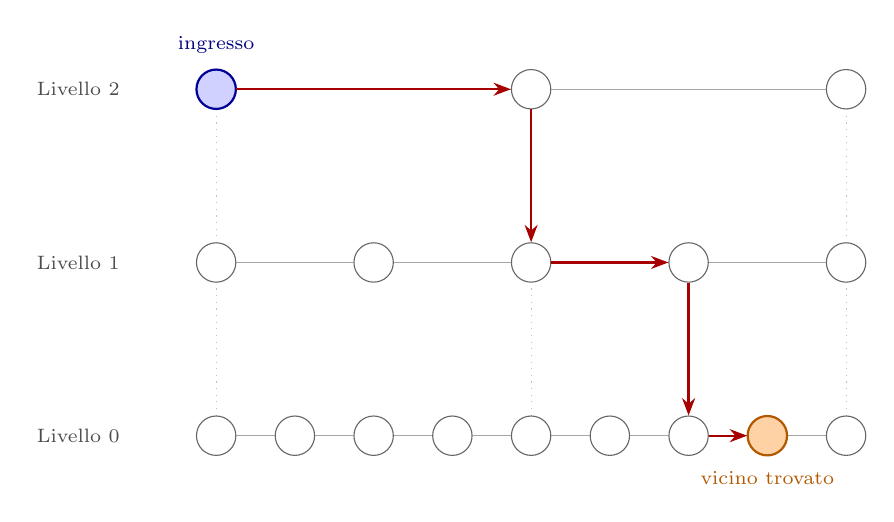
\begin{tikzpicture}[
      node/.style={draw, circle, minimum size=0.5cm, inner sep=0pt, black!60, fill=white},
      entry/.style={node, fill=blue!18, draw=blue!60!black, thick},
      hit/.style={node, fill=orange!35, draw=orange!70!black, thick},
      lyedge/.style={black!35, thin},
      samecol/.style={black!25, thin, dotted},
      srch/.style={-{Stealth[length=2.2mm]}, thick, red!65!black},
      lylabel/.style={font=\scriptsize, black!70, anchor=east},
    ]
    \foreach \x in {0,4,8} \draw[samecol] (\x,0) -- (\x,4.4);

    \foreach \x/\name in {0/p0,1/p1,2/p2,3/p3,4/p4,5/p5,6/p6,7/p7,8/p8}
      \node[node] (\name) at (\x,0) {};
    \draw[lyedge] (p0)--(p1)--(p2)--(p3)--(p4)--(p5)--(p6)--(p7)--(p8);
    \node[hit] at (p7) {};
    \node[lylabel] at (-1.1,0) {Livello 0};

    \foreach \x/\name in {0/m0,2/m2,4/m4,6/m6,8/m8}
      \node[node] (\name) at (\x,2.2) {};
    \draw[lyedge] (m0)--(m2)--(m4)--(m6)--(m8);
    \node[lylabel] at (-1.1,2.2) {Livello 1};

    \foreach \x/\name in {0/t0,4/t4,8/t8}
      \node[node] (\name) at (\x,4.4) {};
    \draw[lyedge] (t0)--(t4)--(t8);
    \node[entry] at (t0) {};
    \node[lylabel] at (-1.1,4.4) {Livello 2};

    \draw[srch] (t0) -- (t4);
    \draw[srch] (t4) -- (m4);
    \draw[srch] (m4) -- (m6);
    \draw[srch] (m6) -- (p6);
    \draw[srch] (p6) -- (p7);

    \node[font=\scriptsize, blue!50!black, above=2pt of t0] {ingresso};
    \node[font=\scriptsize, orange!70!black, below=2pt of p7] {vicino trovato};
  \end{tikzpicture}
  \caption{Ricerca del vicino più prossimo nel grafo HNSW (schematico): dal punto di ingresso nel livello più rado
  (Livello 2), la ricerca scende un livello alla volta muovendosi verso il nodo più vicino alla domanda a ogni
  passo, fino a raggiungere il livello più fitto (Livello 0, tutti i punti) ed esplorarne l'intorno. Le linee
  tratteggiate verticali collegano lo stesso punto presente su più livelli.}
  \label{fig:hnsw}
\end{figure}


\section{Componente di retrieval}\label{sec:retrieval}

A ogni domanda, il componente Retrieving deve individuare, tra i circa 2.500 frammenti indicizzati nel prototipo
(Sezione~\ref{sec:chunking}), i pochi davvero pertinenti da passare al modello generativo. Non è un singolo passo,
ma un imbuto a più stadi, via via più costosi e più precisi (Figura~\ref{fig:imbuto-retrieval}): prima la domanda
viene analizzata e, se necessario, riformulata; poi una ricerca ibrida seleziona un primo insieme ampio di
candidati; un modello di riordinamento li valuta uno a uno contro la domanda; infine i frammenti vengono fusi con
il loro contesto quando serve e filtrati per pertinenza. Questa sezione ne descrive l'adattamento concreto al dominio universitario.

\begin{figure}[H]
  \centering
  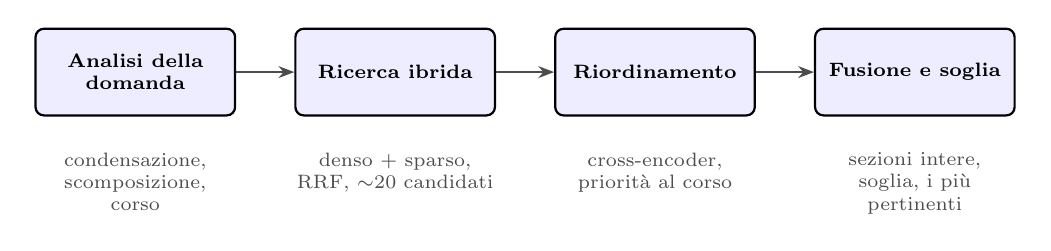
\begin{tikzpicture}[
      stg/.style={draw, thick, rounded corners=3pt, fill=blue!7, align=center, text width=2.3cm,
                  minimum height=1.1cm, font=\scriptsize\bfseries},
      sub/.style={font=\scriptsize, align=center, text=black!70, text width=2.5cm, anchor=north},
      arr/.style={-{Stealth[length=2mm]}, thick, black!70},
    ]
    \node[stg] (q) at (0,0) {Analisi della domanda};
    \node[stg] (hs) at (3.3,0) {Ricerca ibrida};
    \node[stg] (rr) at (6.6,0) {Riordinamento};
    \node[stg] (am) at (9.9,0) {Fusione e soglia};
    \foreach \a/\b in {q/hs, hs/rr, rr/am} \draw[arr] (\a) -- (\b);
    \node[sub] at (0,-0.9) {condensazione, scomposizione, corso};
    \node[sub] at (3.3,-0.9) {denso + sparso, RRF, $\sim$20 candidati};
    \node[sub] at (6.6,-0.9) {cross-encoder, priorità al corso};
    \node[sub] at (9.9,-0.9) {sezioni intere, soglia, i più pertinenti};
  \end{tikzpicture}
  \caption{I quattro stadi del recupero, ciascuno descritto in questa sezione. Un quinto meccanismo, HyDE,
  interviene solo quando il corso è noto e la ricerca ibrida non restituisce
  nulla.}
  \label{fig:imbuto-retrieval}
\end{figure}

\subsection{Analisi della domanda}\label{sec:analisi-domanda}

Prima di essere cercata, la domanda viene normalizzata in tre passi indipendenti. Il primo, la
\emph{condensazione}, riformula una domanda di follow-up in una domanda autonoma alla luce della cronologia della
conversazione, così che il recupero non debba mai cercare un
riferimento implicito. Il secondo, la \emph{scomposizione}, divide una domanda che unisce più richieste distinte in
altrettante domande autonome, cercate e poi fuse separatamente, perché il riordinamento valuta la pertinenza di un
frammento rispetto alla domanda intera, e un frammento pertinente a una sola delle due richieste rischia di uscire
dai primi posti quando l'altra richiesta, nello stesso testo, pesa quanto lei. Entrambe le tecniche sono discusse
nella Sezione~\ref{sec:rag}; nella pratica di questo sistema, la scomposizione richiede un'attenzione che la sola
teoria non rende evidente: quando una richiesta della domanda originale dipende implicitamente da quella
precedente, la domanda scomposta
deve ripetere esplicitamente a quale contesto fa riferimento: senza quel riferimento esplicito, la domanda potrebbe risultare
ambigua quanto quella originale. La stessa chiamata riconosce anche i messaggi che non sono domande
sull'università, come i saluti, che non vengono cercati e ricevono direttamente una risposta.

Il terzo passo, specifico di questo dominio, individua il corso di laurea nominato esplicitamente nella domanda.

Ad esempio, su una cronologia in cui lo studente ha già chiesto ``Entro quando scade il pagamento della
prima rata per gli studenti iscritti a una laurea triennale?'', la nuova domanda ``E per chi è iscritto alla magistrale, e quanto costa la mora se pago in ritardo?'' --- un follow-up che è anche una domanda composta --- viene
prima condensata dal modello linguistico in produzione in ``Ed entro quando scade il
pagamento della prima rata per gli studenti di laurea magistrale, e quanto costa la mora se pago
in ritardo?'', e poi scomposta nelle due domande autonome
\begin{quote}
  \small
  Entro quando scade il pagamento della prima rata per gli studenti di laurea magistrale?\\
  Quanto costa la mora se pago in ritardo la prima rata della laurea magistrale?
\end{quote}
cercate e fuse separatamente nello stadio successivo.

\subsection{Ricerca ibrida}\label{sec:ricerca-ibrida}

Alla domanda, già normalizzata (Sezione~\ref{sec:analisi-domanda}), si applica lo stesso modello di embedding usato
in indicizzazione (Sezione~\ref{sec:embedding}), e Qdrant esegue due ricerche in parallelo, una per la
rappresentazione densa e una per quella sparsa, fondendole con Reciprocal Rank Fusion (Sezione~\ref{sec:rag}). Quando il corso di laurea dello studente è noto, un filtro restringe la ricerca ai soli
frammenti di ateneo e a quelli di quel corso --- gli altri corsi, pur presenti nell'indice, non vengono nemmeno
candidati in questa fase. È una scelta deliberata, non solo un'ottimizzazione: più corsi pubblicano pagine quasi
omonime su argomenti analoghi, con contenuto diverso (ciascuno ha una propria \emph{Prova Pratica Valutativa}, una
propria pagina \emph{Tasse ed esenzioni}), e lasciarle tutte in gara rischierebbe di citare, nella stessa risposta,
requisiti o importi di corsi diversi. Quando il corso non è ancora noto, la ricerca resta invece ristretta alle sole
pagine di ateneo, finché la domanda --- o la pagina trovata --- non permette di risolverlo.
Il risultato di questa fase è un insieme di circa venti candidati, troppi per essere affidabili singolarmente ma
abbastanza pochi da poter essere valutati uno a uno nello stadio successivo.

Per la seconda delle due domande scomposte nell'esempio della Sezione~\ref{sec:analisi-domanda} --- ``Quanto costa
la mora se pago in ritardo la prima rata della laurea magistrale?'' --- ristretta al corso di Psicologia
Scolastica e di Comunità, la ricerca ibrida restituisce effettivamente venti candidati: il punteggio di fusione
decresce da 0,700 del primo a 0,159 dell'ottavo, un calo che mostra perché affidarsi al solo primo risultato della
ricerca ibrida sarebbe rischioso, ma anche perché valutare uno a uno con un modello più accurato solo una ventina di
candidati, invece di migliaia, resta praticabile a ogni domanda.

\subsection{Riordinamento e corso di laurea}\label{sec:corso-priorita}

I candidati della ricerca ibrida vengono valutati da un cross-encoder, \texttt{bge-reranker-v2-m3}
(Sezione~\ref{sec:rag}), che riceve la domanda e ciascun candidato insieme e ne stima la pertinenza reciproca --- più
accurato della sola similarità vettoriale, perché può cogliere corrispondenze specifiche tra i due testi che la
ricerca ibrida, confrontando rappresentazioni calcolate separatamente, non vede. Il candidato non è giudicato sul
solo testo del frammento, ma sul percorso delle sue intestazioni (Sezione~\ref{sec:chunking}) seguito dal testo,
esattamente come già avviene per l'embedding (Sezione~\ref{sec:embedding}): un frammento che è solo una tabella o un
elenco puntato, senza contesto, è spesso incomprensibile al cross-encoder da solo --- per la domanda ``Sotto quale
ISEE si ha l'esenzione?'', il punteggio del frammento ``l'indicatore \dots{} è pari o inferiore a 27.000 €'', che da
solo non dice a cosa si riferisca quella soglia, passa da 0,733 a 0,860 quando gli viene anteposta l'intestazione
della sua sezione. Se il corso di laurea è noto, prima
del riordinamento il suo nome viene rimosso dal testo della domanda: la ricerca è già ristretta a quel corso
(Sezione~\ref{sec:ricerca-ibrida}), e lasciarlo nella domanda farebbe sì che il cross-encoder, un modello sensibile
alla sovrapposizione lessicale, premiasse ogni frammento che nomina quel corso indipendentemente dal contenuto. Un
secondo meccanismo, un bonus fisso di 0,1 al punteggio dei frammenti del corso noto, interviene dopo il riordinamento: a
quel punto, con la ricerca già ristretta al solo corso noto e alle pagine di ateneo, il bonus non serve più a
tenere testa ad altri corsi --- non ce ne sono --- ma a preferire, quando entrambe compaiono tra i candidati, la
versione specifica del corso di un argomento rispetto alla versione generica di ateneo sullo stesso argomento.

Resta il caso in cui il recupero, ristretto al corso noto e alle pagine di ateneo, non trovi nulla sopra la soglia
nemmeno dopo un secondo tentativo con HyDE: può darsi che la domanda riguardi un altro
corso. In questo caso il sistema non prova a cercare da solo tra gli altri
corsi, ma lo chiede esplicitamente allo studente, offrendogli l'elenco dei corsi indicizzati; se lo studente ne
indica uno diverso, la ricerca riparte ristretta al nuovo corso.

Allo studente viene chiesto di indicare il proprio corso anche quando non è ancora noto affatto, ma per una ragione
diversa dalla precedente. In questo caso la ricerca usata per rispondere resta sempre ristretta alle sole pagine di
ateneo (Sezione~\ref{sec:ricerca-ibrida}): non è mai lei a cercare tra i corsi. Se non trova nulla sopra soglia,
allo studente viene chiesto il corso direttamente, come nel caso precedente. Se invece trova qualcosa, il sistema
lancia un'ulteriore ricerca, questa volta senza alcuna restrizione --- su tutto il corpus, corsi compresi --- usata
solo per un confronto e mai per rispondere: se tra i suoi risultati una pagina di un corso specifico ottiene un
punteggio più alto del miglior risultato trovato tra le sole pagine di ateneo, è segno che la domanda dipende da un
corso più di quanto le pagine generali possano dire, e anche in questo caso il sistema preferisce chiedere allo
studente il proprio corso piuttosto che rispondere con un contenuto di ateneo che potrebbe non riguardarlo.

\subsection{Fusione gerarchica e soglia di accettazione}

I frammenti riordinati attraversano infine l'\emph{AutoMergingRetriever} (Sezione~\ref{sec:rag}): quando abbastanza
fratelli della stessa sezione compaiono tra i candidati, vengono sostituiti dalla sezione intera che li contiene
(Sezione~\ref{sec:chunking}), così che il modello generativo riceva un contesto completo invece di frammenti
isolati e lessicalmente vicini tra loro. Solo a questo punto, sui nodi --- frammenti o sezioni fuse --- così
ottenuti, viene applicata una soglia minima di punteggio, 0,3 sui punteggi del riordinamento normalizzati tra 0 e
1: chi non la supera viene scartato, perché un contesto
debolmente pertinente, passato comunque al modello, aumenta il rischio di una risposta costruita su un frammento
sbagliato ma presente, invece di un'astensione corretta --- coerente con il vincolo
di precisione fattuale che guida l'intero sistema (Capitolo~\ref{cap:architettura}). Se nessun nodo raggiunge quella
soglia, un meccanismo di ripiego ne accetta comunque alcuni con una soglia più permissiva, 0,12, piuttosto che
restituire un contesto vuoto: un contesto vuoto forza il rifiuto anche nei casi in cui un frammento scartato dalla
soglia principale fosse in realtà quello giusto, solo formulato in un lessico che il riordinamento premia meno di
quanto meriterebbe. Questo non vuol dire accettare il rischio di una risposta sbagliata al posto di un'astensione:
il modello generativo resta comunque istruito a dichiarare esplicitamente quando il contesto ricevuto non contiene
la risposta, invece di inventarla, ed è questo secondo controllo --- più accurato
perché legge il testo del frammento invece del solo punteggio --- a decidere se un candidato del ripiego risponde
davvero o va scartato. Il ripiego allarga quindi l'insieme dei candidati sottoposti a quel controllo, senza
sostituirlo: la soglia più permissiva decide solo cosa il modello generativo può vedere, non cosa deve usare. Dei
nodi che superano la soglia, solo i più pertinenti vengono infine passati al modello generativo, in ordine di
punteggio decrescente.

\subsection{Recupero di riserva con HyDE}\label{sec:hyde-retrieval}

Quando il corso di laurea è noto ma la ricerca ibrida non restituisce alcun candidato sopra soglia, la domanda viene
cercata una seconda volta con HyDE (Sezione~\ref{sec:rag}): un paragrafo ipotetico, scritto dal modello linguistico
nel linguaggio amministrativo che una vera pagina d'ateneo userebbe, viene accodato alla domanda originale prima di
calcolarne l'embedding. Il caso tipico che questo risolve è un disallineamento di vocabolario tra lo studente e la
pagina che gli risponderebbe: una domanda sul ``test d'ingresso'' cercata contro una pagina che parla di ``prova di
ammissione'' ottiene comunque un punteggio alto nella ricerca densa, che coglie la vicinanza di significato, ma un
punteggio quasi nullo dal cross-encoder, contro lo 0,99 ottenuto dalla stessa pagina quando la query usa il
suo stesso lessico: resta sotto soglia, nonostante
il frammento giusto fosse stato trovato. Il paragrafo ipotetico, scritto con il lessico amministrativo atteso,
porta nella query proprio quella terminologia, mentre la domanda originale resta anch'essa nella query cercata, così
che il riordinamento continui a valutare la pertinenza rispetto a quanto è stato effettivamente chiesto. Al modello
non viene chiesto di essere accurato, solo verosimile nel linguaggio: le date che scrive non vengono mai mostrate
allo studente e servono solo a orientare la ricerca verso il lessico giusto.

La Figura~\ref{fig:hyde-esempio} ripercorre l'intero meccanismo su un caso reale: la domanda ``Quando si tiene il
test d'ingresso?'', il paragrafo ipotetico generato dal modello in produzione per quella domanda, e un frammento
realmente indicizzato --- la pagina del corso di Infermieristica sulla \emph{prova di ammissione} --- contro cui
entrambe le query vengono valutate dal cross-encoder. Senza HyDE, la domanda originale ottiene un punteggio di
0,03, ben sotto la soglia di accettazione; la query completata con il paragrafo ipotetico ottiene invece 0,94,
abbondantemente sopra soglia, pur non avendo il modello azzeccato il termine ``ammissione'' usato dalla pagina: la
sola maggiore ricchezza lessicale e informativa del paragrafo, nel linguaggio amministrativo atteso, è bastata a
farlo riconoscere come pertinente.

\begin{figure}[H]
  \centering
  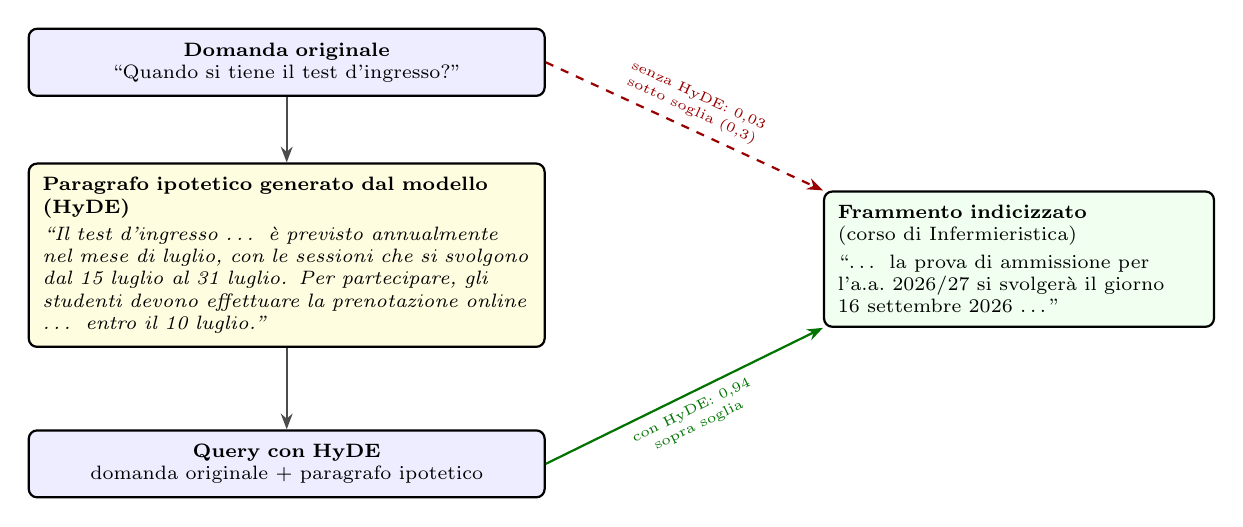
\begin{tikzpicture}[
      box/.style={draw, thick, rounded corners=3pt, text width=6.2cm, font=\scriptsize, inner sep=5pt},
      lbl/.style={font=\tiny, align=center, text width=2.6cm},
      arr/.style={-{Stealth[length=2mm]}, thick},
    ]
    \node[box, fill=blue!7, align=center] (q) at (0,3.6)
      {\textbf{Domanda originale}\\ ``Quando si tiene il test d'ingresso?''};
    \node[box, fill=yellow!12, align=left] (hyde) at (0,1.15)
      {\textbf{Paragrafo ipotetico generato dal modello (HyDE)}\\[2pt]
       \itshape ``Il test d'ingresso \dots{} è previsto annualmente nel mese di luglio, con le sessioni che si
       svolgono dal 15 luglio al 31 luglio. Per partecipare, gli studenti devono effettuare la prenotazione
       online \dots{} entro il 10 luglio.''};
    \node[box, fill=blue!7, align=center] (qf) at (0,-1.5)
      {\textbf{Query con HyDE}\\ domanda originale + paragrafo ipotetico};
    \node[box, fill=green!6, align=left, text width=4.6cm] (page) at (9.3,1.1)
      {\textbf{Frammento indicizzato}\\ (corso di Infermieristica)\\[2pt]
       ``\dots{} la prova di ammissione per l'a.a.\ 2026/27 si svolgerà il giorno 16 settembre 2026 \dots{}''};

    \draw[arr, black!70] (q) -- (hyde);
    \draw[arr, black!70] (hyde) -- (qf);

    \draw[arr, red!60!black, dashed] (q.east) -- (page.north west)
      node[lbl, midway, above, sloped] {senza HyDE: 0,03\\ sotto soglia (0,3)};
    \draw[arr, green!45!black] (qf.east) -- (page.south west)
      node[lbl, midway, below, sloped] {con HyDE: 0,94\\ sopra soglia};
  \end{tikzpicture}
  \caption{Esempio reale del recupero di riserva con HyDE: la domanda originale, cercata da sola contro il
  frammento corretto, ottiene dal cross-encoder un punteggio troppo basso per superare la soglia; la stessa domanda,
  completata con il paragrafo ipotetico generato dal modello, lo supera ampiamente. Punteggi calcolati eseguendo dal
  vivo il reranker e il modello di HyDE in produzione contro un frammento reale dell'indice.}
  \label{fig:hyde-esempio}
\end{figure}


\section{Componente di generazione (LLM)}\label{sec:generazione}

Il componente Generation riceve la domanda e i frammenti selezionati dal recupero e produce la risposta mostrata allo
studente, con l'elenco delle fonti da cui è tratta. È l'unico punto del sistema in cui il testo viene scritto anziché
cercato, e quindi l'unico in cui un'informazione può essere inventata: le scelte descritte in questa sezione ---
il modello, le istruzioni che riceve, il comportamento quando non ha elementi per rispondere --- sono orientate a ridurre questo rischio e a renderlo verificabile, coerentemente con il vincolo di
precisione fattuale introdotto all'inizio del capitolo.

\subsection{Scelta del modello}\label{sec:scelta-modello}

Il modello di produzione è Qwen2.5-14B-Instruct, scelto tra i quattro candidati presentati nella
Sezione~\ref{sec:llm} (Tabella~\ref{tab:llm_comparison}), tutti in versione quantizzata a 4 bit (AWQ) per
rientrare nei 16~GB della GPU dedicata e serviti da vLLM~\cite{kwon2023vllm}. La scelta si basa su un confronto
sperimentale tra i candidati, in cui è il modello che risponde in modo più corretto;
il prezzo è una latenza maggiore rispetto ai candidati più piccoli, ritenuta accettabile a fronte del vincolo di
precisione fattuale. Poiché il modello è servito da vLLM con un nome logico fisso, sostituirlo con uno dei candidati
alternativi richiede solo di cambiare la configurazione.

Il modello genera a temperatura zero, cioè scegliendo sempre la parola più probabile: in un compito in cui la
risposta deve riportare fedelmente un contenuto dato, la variabilità introdotta dal campionamento non porta alcun
beneficio, e la generazione deterministica rende riproducibili sia le risposte sia le valutazioni.

\subsection{Struttura del prompt}\label{sec:prompt}

Il modello riceve una conversazione composta da tre parti (Figura~\ref{fig:prompt}): un messaggio di sistema con le
istruzioni, fisso per ogni domanda; i turni precedenti della conversazione, fino agli ultimi cinque; e il messaggio
dello studente, che il sistema costruisce unendo i frammenti recuperati, il corso dello studente, se noto, e la
domanda.

\begin{figure}[H]
  \centering
  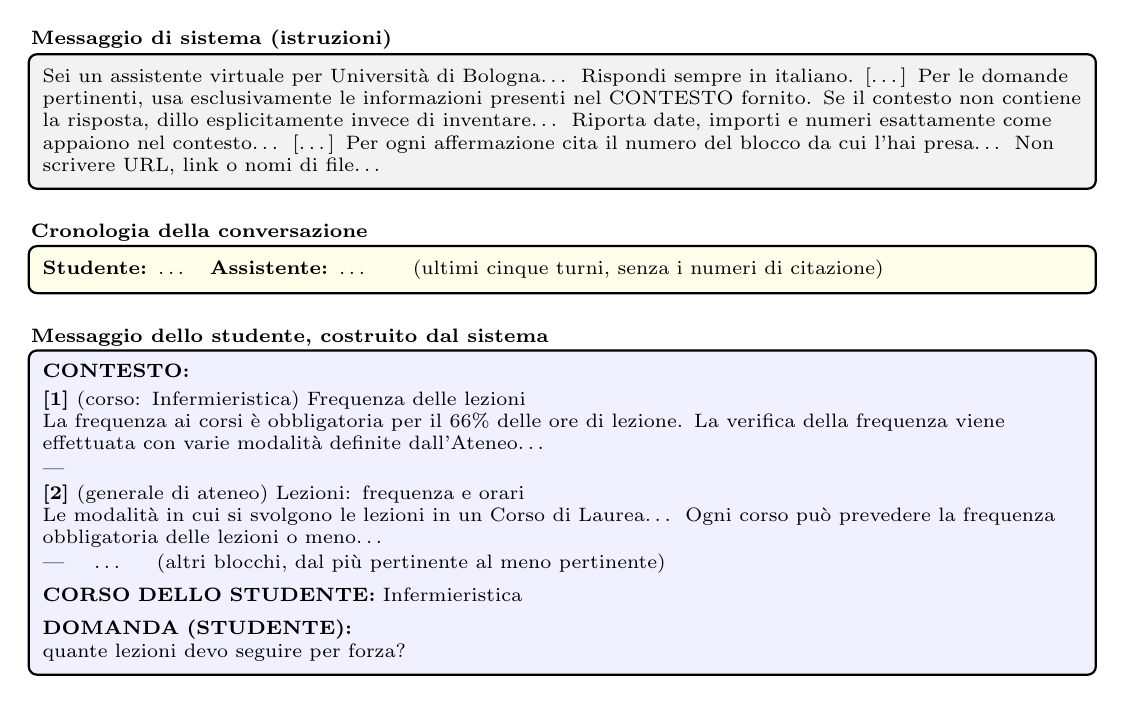
\begin{tikzpicture}[
      part/.style={draw, thick, rounded corners=3pt, align=left, text width=13.2cm, font=\scriptsize, inner sep=5pt},
      tag/.style={font=\scriptsize\bfseries, anchor=south west, inner sep=1pt},
      note/.style={font=\scriptsize\itshape, text=black!65, anchor=west, align=left, text width=3.0cm},
    ]
    \node[part, fill=gray!10] (sys) at (0,0) {%
      Sei un assistente virtuale per Università di Bologna\dots{} Rispondi sempre in italiano. [\dots]
      Per le domande pertinenti, usa esclusivamente le informazioni presenti nel CONTESTO fornito. Se il contesto
      non contiene la risposta, dillo esplicitamente invece di inventare\dots{} Riporta date, importi e numeri
      esattamente come appaiono nel contesto\dots{} [\dots] Per ogni affermazione cita il numero del blocco da cui
      l'hai presa\dots{} Non scrivere URL, link o nomi di file\dots};
    \node[tag] at (sys.north west) {Messaggio di sistema (istruzioni)};

    \node[part, fill=yellow!8, below=7mm of sys] (hist) {%
      \textbf{Studente:} \dots\quad \textbf{Assistente:} \dots\qquad (ultimi cinque turni, senza i numeri di
      citazione)};
    \node[tag] at (hist.north west) {Cronologia della conversazione};

    \node[part, fill=blue!6, below=7mm of hist] (user) {%
      \textbf{CONTESTO:}\\[2pt]
      \textbf{[1]} (corso: Infermieristica) Frequenza delle lezioni\\
      La frequenza ai corsi è obbligatoria per il 66\% delle ore di lezione. La verifica della frequenza viene
      effettuata con varie modalità definite dall'Ateneo\dots\\[1pt]
      ---\\[1pt]
      \textbf{[2]} (generale di ateneo) Lezioni: frequenza e orari\\
      Le modalità in cui si svolgono le lezioni in un Corso di Laurea\dots{} Ogni corso può prevedere la frequenza
      obbligatoria delle lezioni o meno\dots\\[1pt]
      --- \quad \dots{} \quad (altri blocchi, dal più pertinente al meno pertinente)\\[4pt]
      \textbf{CORSO DELLO STUDENTE:} Infermieristica\\[4pt]
      \textbf{DOMANDA (STUDENTE):}\\
      quante lezioni devo seguire per forza?};
    \node[tag] at (user.north west) {Messaggio dello studente, costruito dal sistema};
  \end{tikzpicture}
  \caption{Struttura del prompt inviato al modello, con un esempio reale: la domanda ``quante lezioni devo seguire
  per forza?'' posta da uno studente di Infermieristica. Ogni frammento è un blocco numerato, preceduto
  dall'indicazione del corso o dell'ateneo e dal titolo della pagina e della sezione da cui proviene.}
  \label{fig:prompt}
\end{figure}

\paragraph{I frammenti.} Ogni frammento diventa un blocco numerato, intestato con il titolo della pagina e della
sezione da cui proviene e con il suo ambito, il corso di laurea o l'indicazione ``generale di ateneo''. Il numero
permette al modello di indicare il blocco da cui trae ogni affermazione, e al sistema di trasformare quei numeri
nell'elenco delle fonti mostrato sotto la risposta, con i titoli e gli indirizzi reali delle pagine; l'ambito permette al modello di distinguere informazioni che,
sulle pagine di corsi diversi, hanno lo stesso titolo ma contenuto diverso. I blocchi sono disposti dal più
pertinente al meno pertinente e la domanda è posta in fondo, dopo di essi: in questo modo il frammento più
pertinente e la domanda occupano le due posizioni del contesto che, come discusso nella
Sezione~\ref{sec:rag} (Figura~\ref{fig:u-curve}), il modello sfrutta meglio. Con pochi blocchi il contesto
resta comunque breve, e l'effetto di un'informazione persa nel mezzo è contenuto.

\paragraph{La domanda.} Il modello non risponde al testo digitato dallo studente, ma alla sua versione condensata
(Sezione~\ref{sec:analisi-domanda}), la stessa usata per il recupero: in questo modo non deve ricostruire da solo a
cosa si riferisca una domanda mal formata rispetto a frammenti recuperati per la domanda esplicita. Quando la
domanda è stata scomposta in più parti, il modello le riceve anche separate e numerate, con l'istruzione di
rispondere a ciascuna: la sola versione condensata può infatti confonderle.

\paragraph{Le istruzioni.} Il messaggio di sistema traduce in regole il vincolo di precisione fattuale e i problemi
osservati durante lo sviluppo. Le principali sono:
\begin{itemize}
  \item \textbf{usare solo il contesto}: le informazioni vanno tratte esclusivamente dai blocchi forniti e, se la
  risposta non c'è, il modello deve dirlo invece di ricorrere alla propria conoscenza generale, che per scadenze e
  importi di un ateneo specifico è inaffidabile per costruzione (Sezione~\ref{sec:problema});
  \item \textbf{riportare i numeri alla lettera}: date, importi e soglie vanno trascritti esattamente come
  compaiono, senza arrotondamenti o parafrasi;
  \item \textbf{non riusare le risposte precedenti}: un'informazione data in un turno precedente vale per la domanda
  attuale solo se è presente anche nel contesto di questo turno, perché in una conversazione che cambia argomento o
  corso il modello tendeva a riproporre dati riferiti a un caso diverso;
  \item \textbf{elencare tutte le casistiche}: se il contesto riporta risposte diverse per situazioni diverse ---
  sessioni di laurea, rate, anni di corso --- e la domanda non specifica la propria, il modello deve elencarle tutte,
  ciascuna con la situazione a cui si riferisce, invece di sceglierne una arbitrariamente;
  \item \textbf{rispettare il corso dello studente}: se il corso è indicato, vanno usati solo i blocchi di quel corso
  e quelli di ateneo; se l'informazione esiste solo per un altro corso, il modello può riportarla, ma dichiarando a
  quale corso si riferisce. Senza questa indicazione, a una domanda sulla prova finale di Ingegneria e scienze
  informatiche il modello aveva risposto con le scadenze di Psicologia, presenti nel contesto con un titolo
  identico;
  \item \textbf{rivolgersi direttamente allo studente}: la risposta non deve nominare ``il contesto'' o ``i blocchi'',
  che sono dettagli del funzionamento interno, e se un'informazione manca deve dire semplicemente che non è
  disponibile nei documenti consultati;
  \item \textbf{citare le fonti}: ogni affermazione va accompagnata dal numero del blocco da cui è tratta.
\end{itemize}

\subsection{Gestione dei casi particolari}\label{sec:casi-particolari}

Non tutti i messaggi richiedono, o permettono, una risposta generata dai documenti. La
Figura~\ref{fig:casi-particolari} riassume come il sistema li distingue.

\begin{figure}[H]
  \centering
  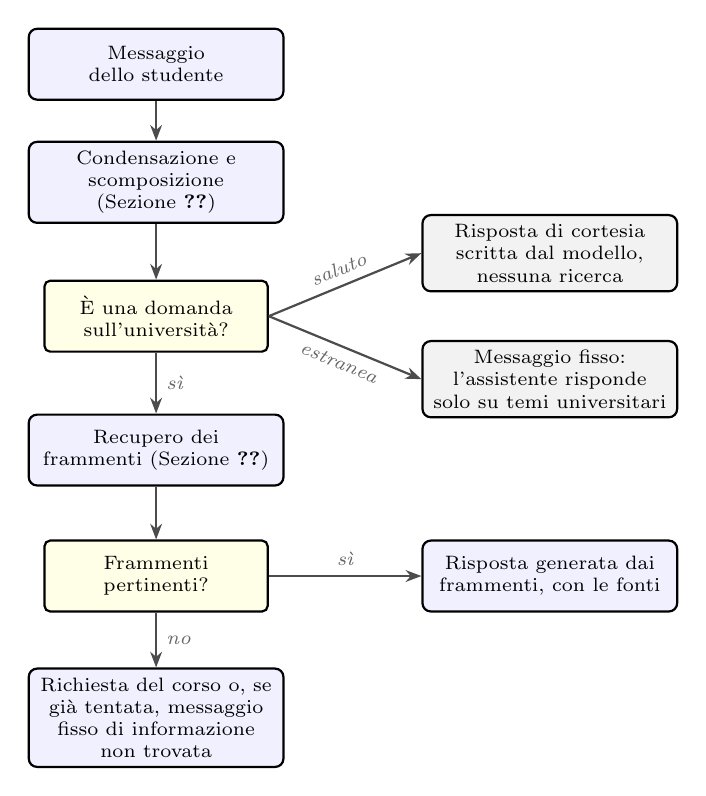
\begin{tikzpicture}[
      dec/.style={draw, thick, rounded corners=2pt, fill=yellow!10, align=center, font=\scriptsize,
                  text width=2.6cm, minimum height=0.9cm},
      act/.style={draw, thick, rounded corners=3pt, fill=blue!6, align=center, font=\scriptsize,
                  text width=3.0cm, minimum height=0.9cm},
      fix/.style={act, fill=gray!10},
      arr/.style={-{Stealth[length=2mm]}, thick, black!70},
      yes/.style={font=\scriptsize\itshape, text=black!60},
    ]
    \node[act] (msg) at (0,0) {Messaggio dello studente};
    \node[act] (an) at (0,-1.5) {Condensazione e scomposizione (Sezione~\ref{sec:analisi-domanda})};
    \node[dec] (kind) at (0,-3.2) {È una domanda sull'università?};
    \node[fix] (smallr) at (5.0,-2.4) {Risposta di cortesia scritta dal modello, nessuna ricerca};
    \node[fix] (topicr) at (5.0,-4.0) {Messaggio fisso: l'assistente risponde solo su temi universitari};
    \node[act] (ret) at (0,-4.9) {Recupero dei frammenti (Sezione~\ref{sec:retrieval})};
    \node[dec] (found) at (0,-6.5) {Frammenti pertinenti?};
    \node[act] (gen) at (5.0,-6.5) {Risposta generata dai frammenti, con le fonti};
    \node[act] (course) at (0,-8.3) {Richiesta del corso o, se già tentata, messaggio fisso di informazione
      non trovata};

    \draw[arr] (msg) -- (an);
    \draw[arr] (an) -- (kind);
    \draw[arr] (kind.east) -- node[yes, above, sloped] {saluto} (smallr.west);
    \draw[arr] (kind.east) -- node[yes, below, sloped] {estranea} (topicr.west);
    \draw[arr] (kind) -- node[yes, right] {sì} (ret);
    \draw[arr] (ret) -- (found);
    \draw[arr] (found) -- node[yes, above] {sì} (gen);
    \draw[arr] (found) -- node[yes, right] {no} (course);
  \end{tikzpicture}
  \caption{Come il sistema tratta un messaggio. I messaggi che non sono domande sull'università vengono riconosciuti
  prima del recupero, dalla stessa chiamata al modello che scompone la domanda; il modello genera una risposta dai
  documenti solo quando il recupero ha trovato frammenti pertinenti.}
  \label{fig:casi-particolari}
\end{figure}

\paragraph{Messaggi che non sono domande.} I saluti e i ringraziamenti (``ciao'', ``grazie mille'') e le domande
estranee all'università (``chi ha vinto la Serie A?'') non devono arrivare al recupero. Cercati come domande, quasi
sempre non trovano nulla, e il sistema chiederebbe allo studente il suo corso di laurea; talvolta trovano invece un
frammento sopra soglia (``buongiorno'' recupera una pagina sulle scuole di specializzazione), che comparirebbe tra
le fonti della risposta.

Il riconoscimento avviene nella scomposizione (Sezione~\ref{sec:analisi-domanda}), senza chiamate aggiuntive al
modello. Prima di scomporre la domanda, il modello stabilisce se il messaggio è un saluto, a cui risponde con una
breve frase cordiale, o se è estraneo all'università, caso in cui il sistema risponde con un messaggio fisso; in
entrambi i casi non si esegue alcuna ricerca. Nel dubbio il messaggio è trattato come una domanda, e lo stesso vale
per un saluto seguito da una domanda (``grazie, e la seconda rata?''). La condensazione, infine, lascia invariati i
messaggi di cortesia, che altrimenti verrebbero riformulati come la domanda precedente.

\paragraph{Nessun frammento pertinente.} Quando il recupero non trova frammenti sopra soglia, nemmeno dopo i
tentativi descritti nella Sezione~\ref{sec:retrieval}, il modello non viene interpellato: la risposta è un messaggio
fisso, che dichiara di non aver trovato l'informazione e suggerisce di rivolgersi al sito o all'ufficio competente.
La scelta di non lasciare la decisione al modello è dettata dall'esperienza: senza contesto, istruito a dire che
l'informazione manca, il modello preferiva comunque formulare una risposta plausibile, arrivando a inventare la
citazione di una fonte inesistente. Prima di arrivare a questo messaggio il sistema chiede allo studente il corso
di laurea, quando la risposta potrebbe trovarsi tra le pagine di un corso (Sezione~\ref{sec:corso-priorita}).

\paragraph{Informazione parzialmente presente.} Il caso più delicato è quello in cui il recupero trova frammenti
pertinenti all'argomento, ma nessuno contiene l'informazione richiesta: una domanda sugli orari di apertura della
biblioteca del campus recupera pagine sulle biblioteche e sui servizi, nessuna delle quali riporta gli orari. Qui la
decisione spetta al modello, che in base alle istruzioni deve dichiarare che l'informazione non è disponibile.
Nelle prove il modello adottato si comporta in questo modo, rispondendo ad esempio che gli orari ``non sono
presenti'' e suggerendo di contattare la biblioteca; talvolta però, contro le istruzioni, si riferisce al
``contesto fornito'', esponendo allo studente un dettaglio del funzionamento interno.


\section{Architettura software e infrastruttura}\label{sec:infrastruttura}

Le sezioni precedenti hanno descritto cosa fa ciascun componente. Questa sezione descrive come il sistema è
realizzato ed eseguito: le tecnologie adottate, la distribuzione dei componenti in servizi, la configurazione e le
misure che rendono l'installazione riproducibile e sicura.

\subsection{Stack tecnologico}

Il sistema è scritto in Python, il linguaggio in cui sono disponibili tutte le librerie dell'ecosistema RAG
utilizzate. La Tabella~\ref{tab:stack} riassume le tecnologie principali e il ruolo di ciascuna.

\begin{table}[H]
  \centering
  \small
  \begin{tabularx}{\textwidth}{>{\raggedright\arraybackslash}p{3.4cm} X}
    \toprule
    \textbf{Tecnologia} & \textbf{Ruolo} \\
    \midrule
    Docling \cite{docling2024} & conversione di PDF, presentazioni e pagine web in documenti strutturati \\
    LlamaIndex & astrazioni comuni per frammenti, docstore, recupero e chiamate al modello linguistico \\
    BGE-M3, bge-reranker-v2-m3 & embedding denso e sparso, riordinamento (libreria FlagEmbedding, PyTorch) \\
    Qdrant & database vettoriale: ricerca ibrida e filtri sui metadati \\
    vLLM \cite{kwon2023vllm} & server di inferenza del modello linguistico e del modello multimodale \\
    Chainlit & interfaccia di chat \\
    RAGAS \cite{es2023ragas} & metriche della valutazione end-to-end \\
    Docker Compose & definizione ed esecuzione dei servizi \\
    pytest & test automatici \\
    \bottomrule
  \end{tabularx}
  \caption{Tecnologie principali del sistema.}
  \label{tab:stack}
\end{table}

Il modello linguistico e il database vettoriale non sono usati come librerie, ma come servizi a cui il resto del
sistema si rivolge attraverso interfacce standard: un'API HTTP compatibile con quella di OpenAI per vLLM, HTTP e
gRPC per Qdrant. Questo rende ciascuno sostituibile senza modificare il codice che lo usa: cambiare il modello
linguistico, come è stato fatto per confrontare i modelli candidati, richiede solo di cambiare un
parametro di configurazione e riavviare il servizio, perché vLLM lo pubblica sempre con lo stesso nome logico.

\subsection{Distribuzione dei componenti}

Il sistema è eseguito come un insieme di servizi containerizzati con Docker, descritti in un unico file di Docker
Compose e rappresentati nella Figura~\ref{fig:deployment}. Tutti i servizi girano sulla stessa macchina e comunicano
attraverso una rete interna, senza alcuna chiamata verso servizi esterni.

\begin{figure}[H]
  \centering
  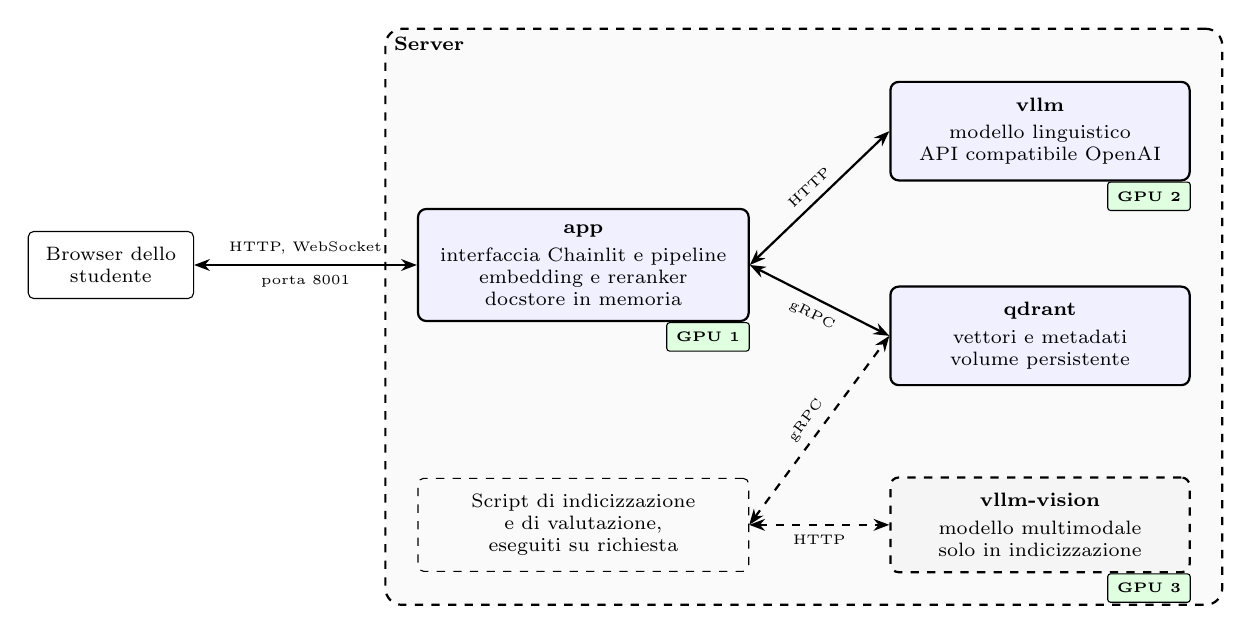
\begin{tikzpicture}[
      svc/.style={draw, thick, rounded corners=3pt, fill=blue!6, align=center, font=\scriptsize,
                  text width=3.4cm, inner sep=2mm},
      opt/.style={svc, dashed, fill=gray!8},
      ext/.style={draw, rounded corners=2pt, align=center, font=\scriptsize, inner sep=2mm},
      gpu/.style={draw, rounded corners=1pt, fill=green!12, font=\tiny\bfseries, inner sep=1.2mm},
      link/.style={{Stealth[length=2mm]}-{Stealth[length=2mm]}, thick},
      lbl/.style={font=\tiny, align=center},
    ]
    \node[ext, text width=1.7cm] (browser) at (-1.0,0) {Browser dello studente};
    \node[svc, text width=3.8cm] (app) at (5.0,0) {\textbf{app}\\[2pt] interfaccia Chainlit e pipeline\\
      embedding e reranker\\ docstore in memoria};
    \node[svc] (vllm) at (10.8,1.7) {\textbf{vllm}\\[2pt] modello linguistico\\ API compatibile OpenAI};
    \node[svc] (qdrant) at (10.8,-0.9) {\textbf{qdrant}\\[2pt] vettori e metadati\\ volume persistente};
    \node[opt] (vision) at (10.8,-3.3) {\textbf{vllm-vision}\\[2pt] modello multimodale\\ solo in indicizzazione};
    \node[ext, dashed, text width=3.8cm] (scripts) at (5.0,-3.3) {Script di indicizzazione e di valutazione,
      eseguiti su richiesta};

    \node[gpu, anchor=north east] at (app.south east) {GPU 1};
    \node[gpu, anchor=north east] at (vllm.south east) {GPU 2};
    \node[gpu, anchor=north east] at (vision.south east) {GPU 3};

    \begin{scope}[on background layer]
      \node[draw, thick, dashed, rounded corners=6pt, fill=black!2, inner sep=4mm,
            fit={(app) (vllm) (vision) (scripts) (12.6,2.6)}] (server) {};
    \end{scope}
    \node[font=\scriptsize\bfseries, anchor=north west] at (server.north west) {Server};

    \draw[link] (browser) -- node[lbl, above] {HTTP, WebSocket} node[lbl, below] {porta 8001} (app);
    \draw[link] (app.east) -- node[lbl, sloped, above] {HTTP} (vllm.west);
    \draw[link] (app.east) -- node[lbl, sloped, below] {gRPC} (qdrant.west);
    \draw[link, dashed] (scripts.east) -- node[lbl, sloped, above] {gRPC} (qdrant.west);
    \draw[link, dashed] (scripts.east) -- node[lbl, below] {HTTP} (vision.west);
  \end{tikzpicture}
  \caption{Distribuzione del sistema su una singola macchina. I servizi in tratto continuo sono sempre attivi;
  quelli tratteggiati solo durante l'indicizzazione o la valutazione, che usano anche il servizio vllm. Ogni
  servizio che usa una GPU ne ha una dedicata.}
  \label{fig:deployment}
\end{figure}

\paragraph{vllm.} Serve il modello linguistico e riceve tutte le richieste a esso rivolte: per ogni domanda la
condensazione, la scomposizione, il riconoscimento del corso e la generazione della risposta, che arriva
all'interfaccia token per token. Le chiamate indipendenti di una stessa domanda vengono inviate in parallelo, e vLLM
le accorpa in un'unica elaborazione sulla GPU (\emph{continuous batching}), come quelle di studenti diversi che
scrivono nello stesso momento: le richieste non si accodano una dopo l'altra.

\paragraph{qdrant.} Conserva i vettori densi e sparsi dei frammenti con i loro metadati. Per ogni domanda, o
sotto-domanda, riceve un'unica richiesta, che esegue la ricerca densa e quella sparsa e ne fonde i risultati direttamente nel database.
I dati risiedono in un volume persistente, che sopravvive al riavvio o all'aggiornamento del container.

\paragraph{app.} Ospita l'interfaccia, la pipeline di risposta e i modelli di embedding e di reranking. Questi ultimi
sono molto più piccoli del modello linguistico e vengono eseguiti nello stesso processo, su una GPU diversa da
quella di vLLM, senza
passare per la rete. Il loro uso è serializzato, perché le librerie che li eseguono non tollerano chiamate
concorrenti; la loro elaborazione dura però una frazione di secondo, contro i secondi della generazione, e non
limita in pratica il numero di studenti serviti. L'indice e i pesi dei modelli non fanno parte dell'immagine del
container, ma vengono montati dal disco della macchina: aggiornare i documenti non richiede di ricostruirla.

\paragraph{vllm-vision.} Serve il modello multimodale che descrive le immagini durante la conversione dei documenti
(Sezione~\ref{sec:ingestione}). Viene avviato solo per l'indicizzazione, su una GPU distinta, e poi spento: il
servizio di risposta resta attivo e il sistema continua a funzionare anche mentre i documenti vengono aggiornati.

L'avvio segue le dipendenze tra i servizi: l'applicazione parte solo quando Qdrant e vLLM risultano pronti, cosa che
per vLLM richiede il caricamento del modello in memoria. Ogni servizio espone un controllo di stato, e Docker
riavvia automaticamente quelli che si interrompono.

\subsection{Configurazione}

Tutti i parametri che dipendono dall'installazione sono raccolti in un unico file di variabili d'ambiente, letto sia
da Docker Compose sia dall'applicazione: indirizzi e porte dei servizi, GPU assegnate a ciascuno, modelli da
caricare, nome della collezione in Qdrant. L'applicazione li legge in un oggetto di configurazione tipizzato, che
fornisce un valore predefinito per ciascuno e segnala all'avvio quelli mancanti o non validi. Nello stesso oggetto
si trovano i parametri della pipeline, come le soglie del recupero, il numero di frammenti passati al modello e la
lunghezza della cronologia, e i dati dell'istituzione (nome dell'ateneo e ambito dell'assistente) usati nei prompt:
adattare il sistema a un'altra configurazione hardware, o a un altro ateneo, non richiede modifiche al codice.

\subsection{Diagnostica e test}

L'interfaccia offre una modalità di diagnostica, selezionabile dalla chat, che mostra lo svolgimento di ogni stadio
della pipeline: la domanda condensata e scomposta, il corso riconosciuto, i frammenti recuperati con il loro
punteggio e il prompt completo inviato al modello. È lo strumento con cui sono stati analizzati i casi problematici
riportati in questo capitolo. Le stesse informazioni vengono registrate nei log dell'applicazione.

La logica che non dipende dai modelli è coperta da test automatici: pulizia delle pagine e suddivisione in
frammenti, estrazione dei metadati, riconoscimento del corso, costruzione del prompt e dell'elenco delle fonti,
metriche di valutazione. Le chiamate al modello linguistico sono sostituite da un modello simulato con risposte
predefinite, così che i test girino in pochi secondi, senza GPU né servizi attivi, e possano essere eseguiti
automaticamente a ogni modifica del codice.



\chapter{Validazione del sistema}\label{cap:validazione}

\section{Benchmark di test}

% TODO: Descrivere il/i dataset o benchmark utilizzati per valutare il sistema: fonte, composizione
% del dataset, criteri di costruzione (se creato ad-hoc), eventuale suddivisione
% train/validation/test, limiti del benchmark scelto.


\section{Indicatori di accuratezza}

% TODO: Definire le metriche usate per valutare le prestazioni del sistema, motivando la scelta
% (es. accuracy, F1, exact match, BLEU/ROUGE, metriche semantiche, metriche specifiche per RAG come
% context precision/recall, faithfulness, answer relevancy).


\section{Esperimenti effettuati}

% TODO: Descrivere in dettaglio gli esperimenti condotti per valutare il sistema, in modo che siano
% riproducibili: obiettivo, setup, parametri usati, baseline di confronto, riproducibilità (seed,
% versioni dei modelli, data di esecuzione).


\section{Risultati}

\subsection{Risultati}

% TODO: Presentare e commentare i risultati ottenuti dagli esperimenti descritti in 4.3: tabelle/grafici
% riassuntivi (salvare grafici in Assets/Immagini/), analisi comparativa, discussione dei risultati
% rispetto alle aspettative/stato dell'arte, analisi statistica se rilevante.


\subsection{Esempi di casi errati}

% TODO: Fornire un'analisi qualitativa degli errori del sistema, utile per capire i limiti attuali e
% orientare sviluppi futuri: domanda/input, risposta corretta attesa, risposta effettivamente
% generata, analisi dell'errore (retrieval vs generazione), categoria dell'errore.




\chapter{Conclusioni e sviluppi futuri}\label{cap:conclusioni}

% TODO: Riassumere il lavoro svolto, i risultati principali ottenuti e indicare le direzioni di
% sviluppo future: riepilogo del problema e della soluzione proposta, principali risultati, limiti
% del lavoro attuale, sviluppi futuri (tecnici, funzionali, passi per il deploy in produzione),
% considerazioni finali.


% ===== Bibliografia (stile IEEE) =====
\bibliographystyle{ieeetr}
\bibliography{bibliografia}

\end{document}
